\documentclass[11pt]{article}
\usepackage[T1]{fontenc}
\usepackage{lmodern}
\usepackage[margin=1.05in]{geometry}
\usepackage{amsmath,amssymb,amsthm,mathtools}
\usepackage{microtype,booktabs,enumitem,xcolor}
\usepackage{tikz}
\usetikzlibrary{arrows.meta,positioning,calc,decorations.pathreplacing,fit,backgrounds}
\usepackage{hyperref}
\hypersetup{colorlinks=true,linkcolor=blue!45!black,citecolor=blue!45!black,
 urlcolor=blue!45!black,pdftitle={Logarithmic Relative Fluctuations in the Weakly Disordered Planar Ising Model},pdfauthor={OpenAI}}
\newtheorem{theorem}{Theorem}[section]
\newtheorem{proposition}[theorem]{Proposition}
\newtheorem{lemma}[theorem]{Lemma}
\newtheorem{corollary}[theorem]{Corollary}
\theoremstyle{definition}
\newtheorem{definition}[theorem]{Definition}
\newtheorem{assumption}[theorem]{Assumption}
\theoremstyle{remark}
\newtheorem{remark}[theorem]{Remark}
\newcommand{\E}{\mathbb E}
\newcommand{\Prob}{\mathbb P}
\newcommand{\R}{\mathbb R}
\newcommand{\Z}{\mathbb Z}
\newcommand{\N}{\mathbb N}
\newcommand{\one}{\mathbf 1}
\newcommand{\eps}{\varepsilon}
\newcommand{\cG}{\mathcal G}
\newcommand{\dd}{\,\mathrm d}
\newcommand{\norm}[1]{\left\lVert#1\right\rVert}
\newcommand{\abs}[1]{\left\lvert#1\right\rvert}
\DeclareMathOperator{\Cov}{Cov}
\DeclareMathOperator{\cum}{cum}
\DeclareMathOperator{\supp}{supp}
\DeclareMathOperator{\dist}{dist}
\numberwithin{equation}{section}
\setlength{\emergencystretch}{1.5em}
\title{Logarithmic Relative Fluctuations in the\texorpdfstring{\\}{ }Weakly Disordered Planar Ising Model}
\author{OpenAI}
\date{October 5, 2026}
\begin{document}
\maketitle
\begin{abstract}
Assuming the stated deterministic critical-reference estimates, we prove
that the relative second moment of the quenched critical spin correlation
in the square-lattice Ising model with independent fair bonds $1\pm\eps$
grows as $(\log r)^{1/4+o(1)}$ for each sufficiently small fixed $\eps>0$.
The correlation is evaluated at the physical critical temperature, with
the thermodynamic limit taken before the disorder moments and the
large-distance limit.
\end{abstract}
\setcounter{tocdepth}{1}
\tableofcontents
\clearpage
\section{Introduction}

Weak random bonds in the planar Ising model provide a basic example in
which disorder is expected to change critical correlations through logarithmic
factors. The fluctuations of a quenched correlation are particularly revealing:
the correlation is first computed in a fixed environment, with its own Gibbs
normalization, and only then averaged over the bonds. This paper establishes
the predicted logarithmic growth of its relative second moment for small,
fixed binary disorder. The proof uses deterministic critical-reference
estimates from~\cite{ReferenceIsing}; the stochastic estimates and the
identification of the physical critical point are proved here.

\subsection{Model and result}

Let $E$ be the unordered nearest-neighbor edges of $\Z^2$, each counted once,
and let $(\xi_e)_{e\in E}$ be independent fair signs on a single probability
space. Fix $0<\eps<1$ and set $J_e(\omega)=1+\eps\xi_e(\omega)$.
For $\Lambda_n=\{-n,\ldots,n\}^2$, define
\begin{align}
 H^{\mathrm f}_{n,\omega}(\sigma)
   &=-\sum_{\substack{e=\{x,y\}\in E\\x,y\in\Lambda_n}}
       J_e(\omega)\sigma_x\sigma_y,\label{eq:free-hamiltonian}\\
 H^+_{n,\omega}(\sigma)
   &=-\sum_{\substack{e=\{x,y\}\in E\\e\cap\Lambda_n\ne\varnothing}}
       J_e(\omega)\sigma_x\sigma_y,
       \qquad \sigma_x=1\quad(x\notin\Lambda_n).
       \label{eq:plus-hamiltonian}
\end{align}
In the second sum, edges wholly outside $\Lambda_n$ are omitted. For
$b\in\{\mathrm f,+\}$ and $\beta\ge0$, write
$\langle\cdot\rangle^b_{n,\beta,\omega}$ for the Gibbs expectation
proportional to $\exp(-\beta H^b_{n,\omega})$. Every expectation is
normalized separately at its indicated environment and boundary condition.

The physical critical inverse temperature is
\begin{equation}\label{eq:critical-definition}
 m_\eps(\beta)=\E\!\left[\lim_{n\to\infty}
       \langle\sigma_0\rangle^+_{n,\beta,\omega}\right],
 \qquad
 \beta_c(\eps)=\inf\{\beta\ge0:m_\eps(\beta)>0\}.
\end{equation}
Ferromagnetic monotonicity gives the plus limit. Comparison with constant
bonds, with $\beta_0=\tfrac12\log(1+\sqrt2)$, gives
\[
 0<\frac{\beta_0}{1+\eps}\le\beta_c(\eps)
       \le\frac{\beta_0}{1-\eps}<\infty.
\]
For each integer $r\ge3$, let
\begin{equation}\label{eq:quenched-correlation}
 C_{\eps,\omega}(r)=\lim_{n\to\infty,\,n\ge r}
       \langle\sigma_0\sigma_{(r,0)}\rangle^{\mathrm f}
                   _{n,\beta_c(\eps),\omega},
 \qquad
 R_\eps(r)=\frac{\E[C_{\eps,\omega}(r)^2]}
                 {\E[C_{\eps,\omega}(r)]^2}.
\end{equation}
The free correlation limit exists by monotonicity in the volume and lies
in $(0,1]$. In particular $R_\eps(r)$ is defined and is at least one.
All unqualified expectations $\E$ below are over the environment; auxiliary
independent random choices used in the proof will be included explicitly
when introduced.

\begin{theorem}\label{thm:main}
Assume the deterministic reference-model estimates of
\cite{ReferenceIsing}, at the scopes stated in Section~\ref{sec:reference}.
There is $\eps_0>0$ such that for every fixed $\eps\in(0,\eps_0)$,
\begin{equation}\label{eq:main-limit}
 \lim_{r\to\infty,\,r\in\N}
       \frac{\log R_\eps(r)}{\log\log r}=\frac14.
\end{equation}
The critical inverse temperature in \eqref{eq:quenched-correlation} is
the physical value \eqref{eq:critical-definition}; it is the unique positive
solution of
\begin{equation}\label{eq:critical-curve}
 \sinh\bigl(2\beta(1-\eps)\bigr)
 \sinh\bigl(2\beta(1+\eps)\bigr)=1.
\end{equation}
\end{theorem}

The order of limits is essential. The disorder strength is fixed first;
the free thermodynamic limit is then taken for each separation, followed
by the disorder moments and the limit in $r$. Constants and errors may
depend on this fixed positive strength. At $\eps=0$ the environment is
deterministic and $R_0(r)=1$.

The reference input concerns deterministic translation-invariant,
square-symmetric, finite-range even perturbations and their critical
nearest-neighbor comparison kernels. It supplies neither a random critical
point nor a quenched moment estimate. Section~\ref{sec:reference} states
the particular reference consequences needed below, including their
buffer and symmetry conditions. The proof of
Theorem~\ref{thm:main} establishes the random estimates from these inputs.

\subsection{Historical context}

The pure planar Ising model has specific-heat exponent zero, the borderline
case left undecided by Harris's criterion for the effect of quenched
disorder~\cite[Section~5]{Harris1974}. Dotsenko and Dotsenko obtained the
double-logarithmic prediction for the random model's specific heat
\cite{DotsenkoDotsenko1983}. Shalaev's renormalization analysis predicted
unchanged leading critical indices~\cite{Shalaev1984}. Shankar and Ludwig
developed the logarithmic corrections to spin-correlation moments
\cite{Shankar1987,Ludwig1990}. In particular, Shankar predicted
the factor $(\log r)^{1/4}$ in the second moment of the spin correlation,
and Ludwig studied logarithmic corrections to its moments. The exponent
in Theorem~\ref{thm:main} is thus an established prediction. The issue
addressed here is its derivation for normalized quenched correlations at
the physical critical point, under the stated reference input.

The deterministic reference theory has a different role. Critical
nearest-neighbor spin correlations and mixed primary fields have rigorous
scaling limits; the limiting fields satisfy operator-product expansions
\cite{CHI2015,CHI2023}. Rigorous results for deterministic weak
perturbations include energy correlations in the plane
\cite{GGM2012}, energy correlations on cylinders~\cite{AGG2023}, and
boundary spin correlations in the half-plane~\cite{CGG2025}. These results
provide context for the deterministic bulk premise used here
\cite{ReferenceIsing}; none supplies the random moment estimates below.
The energy and spin operator products enter the coefficient computation
in Section~\ref{sec:coefficients}, after the local estimates needed for
random interactions have been established.

Rigorous critical behavior at a self-dual random-bond law also predates
this work. Building on disorder-rounding results of Aizenman and Wehr
\cite{AizenmanWehr1990}, Chayes and Shtengel proved zero magnetization
and algebraic lower bounds on averaged correlations at the binary
self-dual law~\cite[Theorems~1$'$ and~2$'$]{ChayesShtengel1999}. Their
argument did not exclude a critical phase containing that point. Here
the weak-disorder estimates identify the tuned parameter with the
physical critical threshold and give the logarithmic moment asymptotic
there. The probabilistic part uses the random-cluster representation
\cite{FK1972,EdwardsSokal1988}, critical crossing estimates
\cite{DHN2011,CDH2016}, product-space influences~\cite{GJN2013}, and the
monotone-measure extension~\cite{DCRT2019} of the decision-tree inequality
of O'Donnell, Saks, Schramm, and Servedio~\cite{OSSS2005}.

\subsection{Proof strategy and the role of locality}

It is convenient to include inverse temperature in the couplings and use
the coordinates
\begin{equation}\label{eq:model-td}
 \log\sinh(2K_e)=t+D\xi_e,\qquad D>0.
\end{equation}
For each sufficiently small fixed $D$, we first choose $t$ by a
renormalization construction. The last part of the proof identifies this
choice with $t=0$ and then returns to the original parameter $\beta$.

At scale $r_j=r_0L^j$, the effective interaction is a sum of local even
spin functions. Each cell has one distinguished term whose size is allowed
to be large. The other terms are indexed by connected sets of cells and
have small norms with exponential decay in the size of those sets. Every
term records both the spins on which it acts and the original random
variables on which its coefficients depend. This second record will give
exact independence of the leading factors attached to well-separated
spin insertions.

The first difficulty is to transport interactions that are small in high
moments but are not uniformly small. Section~\ref{sec:blocking} constructs
an exact local change of representation. An isolated group of large
interactions is integrated as a positive exponential weight. Insertions
in the same region are transported by its normalized conditional law.
Reference comparison across a surrounding buffer bounds the resulting
density, and reference even-function decay attenuates its dependence on
the outer spins. Failures of this attenuation have a distant large-field
witness, which can be paid for using independence and high moments.
Section~\ref{sec:norms} turns these observations into the estimates needed
to iterate the construction. In particular, it controls mixed moments of
spin sources and nearby background fields, whose randomness is shared.

The linearized background transport has one expanding mean coordinate
and one neutral covariance coordinate. The first is removed by choosing
$t$; the second, denoted $g_j$, measures thermal-charge variance per unit
area. Section~\ref{sec:linear} proves contraction of the remaining
coordinates. The nonlinear coefficients of the two surviving effects are
computed in Section~\ref{sec:coefficients}. Its method uses finitely many
microscopic energy insertions: exact partition identities preserve their
normalized charges, and the reference energy and spin operator products
determine the logarithmic terms. Only finite-degree polynomial calculations
are needed. This separates the coefficient calculation from the estimates
that justify the real random iteration.

The resulting flow, proved in Sections~\ref{sec:flow} and~\ref{sec:marked},
satisfies $g_j\sim(B_0j)^{-1}$ for a positive constant $B_0$. The leading
random factor of a transported spin has a bounded positive mean and
second moment $j^{1/8+o(1)}$. Two distant insertions have independent
leading factors once their small nonlocal remainders are removed.
Section~\ref{sec:readout} uses an enlarging terminal buffer to compare
the remaining Gibbs expectation with the critical reference expectation.
It obtains the relative second-moment exponent $1/4$ and also a high-moment
wired-arm bound.

Finally, Section~\ref{sec:transition} identifies the physical transition.
Twisted torus partition functions locate the tuned value at the
distributionally self-dual point. A product-space influence inequality
and a random-shell exploration inequality make the needed threshold and
subcritical estimates explicit. Planar random-cluster duality then gives
positive magnetization above tuning. This final step connects the local
renormalization construction to the critical point used in the statement.

The reusable parts of the method are the positive treatment of large
local interactions, the simultaneous tracking of spin support and random
dependence, and the extraction of marginal coefficients from invariant
charges of finitely many insertions. Their application here requires all
three: locality controls dependence, high moments control exceptional
fields, and the coefficient identities determine the logarithmic exponent.

\section{Reference averaging, charges, and field products}\label{sec:reference}

The changes of scale below use conditional expectations in the critical
nearest-neighbor model.  This section records their precise scope and derives
three consequences: an invariant coefficient for each of the energy and spin
directions, the large-distance coefficients of the products of these fields,
and a finite set of boundary tests that controls an averaged sup norm.  These
are deterministic statements.  Estimates for the random lists constructed
from them begin in Section~\ref{sec:norms}.

\subsection{The reference measure and its accepted inputs}

Write $\langle\cdot\rangle_0$ for critical nearest-neighbor plane expectation
on $\Z^2$, at coupling $K_c=\frac12\log(1+\sqrt2)$.  For a max-norm square
$B_R(z)$, let $P_{R,z}$ be conditional expectation over its interior, retaining
the spins of its cutting contour.  Thus $P_{R,z}F$ is a function of cutting
spins whenever $F$ is supported inside the square.  All sup norms in this
section are over every assignment of the spins on the support of the
function; for $P_{R,z}F$ these are the cutting spins.  We abbreviate
$P_{R,0}$ to $P_R$.  Nested cuts compose by the tower property.  In particular,
if a square lies inside a larger reference domain, replacing an observable
inside the square by its conditional average preserves its expectation in
that domain, as well as in the plane.

Put $F^\circ=F-\langle F\rangle_0$, and use this representative for even
functions modulo constants.  An odd function already has plane mean zero.
Our scalar energy and spin dimension are
\begin{equation}\label{ref:energy}
 e(z)=\frac14\sum_{v:\,|v-z|=1}
       \bigl(\sigma_z\sigma_v-\langle\sigma_z\sigma_v\rangle_0\bigr),
 \qquad d=\frac18.
\end{equation}
We use Euclidean distances for field asymptotics and max-norm squares for
conditional averaging.  This distinction changes no buffer condition.

The supplied conformal-universality theorem applies to a fixed deterministic
potential on finite even sets, of fixed finite range, invariant under lattice
translations, reflections, and right-angle rotations.  For a sufficiently
small fixed coefficient multiplying that potential, it supplies a critical
branch, nonzero field factors, and separated bulk spin and energy limits in
smooth simply connected domains with free, plus, or minus boundary, and in
the plane obtained from periodic-square thermodynamic limits
\cite[Theorem~1.1]{ReferenceIsing}.  We use its conditional
averaging, thermal, and marked-source interfaces only for the unperturbed
critical reference model in bulk charts with their prescribed buffers.
In particular, its conditional kernels throughout this paper are $P$;
they are never conditional kernels of a random effective interaction.

Here are the specific operator and calibration inputs.  If $F$ is supported
in $B_w(0)$, set
\begin{equation}\label{ref:disk-response}
 d_R(F)=\langle F\rangle^+_{\mathrm{disk}(4R)}-\langle F\rangle_0.
\end{equation}
For each sufficiently large fixed ratio $R/w$, and all sufficiently large
$w$, the reference estimate gives
\begin{align}
 |d_R(F)|&\le C(w/R)^b\norm{F}_\infty,
 \label{ref:response-input}\\
 \norm{P_RF^\circ}_\infty
   &\le C|d_R(F)|+C(w/R)^p\norm{F}_\infty,
 \label{ref:operator-input}
\end{align}
where
\begin{equation}\label{ref:exponents}
 (b,p)=
 \begin{cases}
  (1,3),&F\text{ is even and invariant under right-angle rotations},\\
  (1,2),&F\text{ is even},\\
  (d,1+d),&F\text{ is odd}.
 \end{cases}
\end{equation}
The constant is uniform over sufficiently large fixed ratios, whereas the
fine-mesh threshold can depend on the ratio.  Ratios converging to a fixed
admissible value are allowed.  The norm bound is uniform over all cutting
configurations \cite[Proposition~4.1]{ReferenceIsing}.

Write $\mathcal O_1(z)=e(z)$ and $\mathcal O_d(z)=\sigma_z$,
and omit $z$ when $z=0$.  There are nonzero
constants $\kappa_b$ such that
\begin{equation}\label{ref:calibration}
 R^b d_R(\mathcal O_b)\longrightarrow\kappa_b.
\end{equation}
Moreover the averaged reference fields satisfy
\begin{equation}\label{ref:line-norms}
 c\le\norm{w^bP_w\mathcal O_b}_\infty\le C,
 \qquad
 c(w/R)^b\le |d_R(w^bP_w\mathcal O_b)|\le C(w/R)^b.
\end{equation}
Here and below energy fields are plane-centered.  These are the calibration
and field-line estimates of
\cite[Lemmas~4.5 and~5.3 and Equation~(5.18)]{ReferenceIsing}.  The exact identity
behind the last reference is
\begin{equation}\label{ref:exact-line}
 B^bP_{Bw}\bigl(w^bP_w\mathcal O_b\bigr)
          =(Bw)^bP_{Bw}\mathcal O_b.
\end{equation}
No convergence rate for primary fields is used in these inputs.

\subsection{Invariant energy and spin coefficients}

The disk response in \eqref{ref:operator-input} depends on the observation
scale.  To use a single thermal coordinate through successive cuts, we first
replace that response by a linear functional invariant under all cuts.

\begin{lemma}[Invariant charges]\label{ref:charges}
There are linear functionals $\ell$ on bounded local even functions modulo
constants and $\ell_s$ on bounded local odd functions with
\[
 \ell(e(z))=1,\qquad \ell_s(\sigma_z)=1.
\]
They commute with translations and square symmetries and are invariant under
reference conditional averaging whenever the cut encloses the support.
For $b=1$ write $\ell_b=\ell$, and for $b=d$ write $\ell_b=\ell_s$; the subscript in
$\ell_s$ means spin.  If $F$ has the corresponding parity and support in a
square of radius $w$ above a fixed threshold, then
\begin{equation}\label{ref:charge-bound}
 |\ell_b(F)|\le Cw^b\norm{F}_\infty,
 \qquad
 \ell_b(F)=\kappa_b^{-1}\lim_{R\to\infty}R^b d_R(F).
\end{equation}
The disk in this limit may be centered at any fixed lattice point.  In the
even case $\ell_b$ annihilates constants.
\end{lemma}

\begin{proposition}[Averaging and charge cancellation]\label{ref:operator}
Fix $\nu>0$ smaller than $p-b$ in the applicable row of
\eqref{ref:exponents}.  For all sufficiently large $w$ and $R\ge Cw$, a
function $F$ of that parity, supported in $B_w(z)$, satisfies
\begin{align}
 \norm{P_{R,z}F^\circ}_\infty
   &\le C(w/R)^b\norm{F}_\infty,\label{ref:ordinary-decay}\\
 \norm{P_{R,z}F^\circ-\ell_b(F)P_{R,z}\mathcal O_b(z)}_\infty
   &\le C(w/R)^{p-\nu}\norm{F}_\infty.
   \label{ref:improved-decay}
\end{align}
In particular, the second bound is the improved decay bound for a function
of charge zero.  We shall use $\nu=1/4$.  The exponent $3-\nu$ requires
the individual even function to be invariant under right-angle rotations;
invariance of its probability law alone does not suffice.
For a site at fixed positive relative distance from the cutting contour,
\begin{equation}\label{ref:microscopic-decay}
 \norm{P_{R,z}e(y)}_\infty\le CR^{-1},\qquad
 \norm{P_{R,z}\sigma_y}_\infty\le CR^{-d}.
\end{equation}
The first bound also holds for a single plane-centered bond product.
\end{proposition}

\begin{proof}[Proof of Lemma~\ref{ref:charges} and
Proposition~\ref{ref:operator}]
Fix a sufficiently large integer $B$ and put $w_k=B^kw$.  In the appropriate
parity space, with plane centering in the even case, define
\[
 v_k=w_k^bP_{w_k}\mathcal O_b,
 \qquad S_k=B^bP_{w_{k+1}}.
\]
The lines $\R v_k$ are uniformly nonzero and bounded by
\eqref{ref:line-norms}, and $S_kv_k=v_{k+1}$ by
\eqref{ref:exact-line}.  If $F$ is supported in $B_{w_k}$, subtract
$\alpha v_k$ to cancel its response in the disk of radius $4w_{k+1}$.
Equations~\eqref{ref:response-input} and \eqref{ref:line-norms} give
$|\alpha|\le C\norm{F}_\infty$.  Applying
\eqref{ref:operator-input} to this difference proves the quotient bound
\begin{equation}\label{ref:quotient}
 \norm{S_k:\,X_k/\R v_k\longrightarrow X_{k+1}/\R v_{k+1}}
       \le CB^{b-p}.
\end{equation}
Here $X_k$ is the space of bounded functions of the required parity on
$B_{w_k}$, with plane mean zero in the even case and with right-angle
rotation invariance imposed when $p=3$; its norm is the sup norm.
The same estimate holds after subtracting any multiple of $v_k$, so it is
indeed an estimate for the quotient norm.  Combining \eqref{ref:response-input} and \eqref{ref:operator-input}
at the fixed ratio $B$ also bounds $S_k$ uniformly.

Choose uniformly bounded projections onto $\R v_k$, using for example
the response in a disk at one fixed large multiple of $w_k$ and dividing
by its nonzero response on $v_k$.  In the resulting bounded splittings,
\[
 S_k=
 \begin{pmatrix}1&\beta_k\\0&D_k\end{pmatrix},\qquad
 \norm{\beta_k}\le C,\quad \norm{D_k}\le CB^{b-p}=:q.
\]
Enlarge $B$ until $q\le B^{b-p+\nu}<1$.  Writing
$S_{k-1}\cdots S_0F=a_kv_k+u_k$ gives
\[
 \norm{u_k}\le Cq^k\norm{F}_\infty,\qquad
 a_{k+1}-a_k=\beta_ku_k.
\]
Consequently $a_k$ converges to a linear functional $a_\infty(F)$ and
\begin{equation}\label{ref:line-limit}
 |a_\infty(F)|\le C\norm{F}_\infty,
 \quad
 \norm{S_{k-1}\cdots S_0F-a_\infty(F)v_k}_\infty
       \le Cq^k\norm{F}_\infty.
\end{equation}
Define $\ell_b(F)=w^ba_\infty(F)$.  Since the line is transported exactly,
its coefficient is one on $\mathcal O_b$.  Constants have already been
removed.  Dividing \eqref{ref:line-limit} by $B^{kb}$ gives
\eqref{ref:improved-decay} at the radii $w_k$ and gives
\eqref{ref:charge-bound}'s bound.  The construction permits an arbitrary
initial function on the first square; it need not initially be a function
of the cutting contour.

To identify the functional independently of the chosen initial scale,
first divide \eqref{ref:line-limit} by $B^{kb}$ and test the resulting
unscaled decomposition in a plus disk at a fixed sufficiently large
multiple of $w_k$.  Conditional averaging preserves that expectation.
After multiplication by the disk scale to the power $b$, the error is
$O(B^{k(b-p+\nu)})$ and tends to zero because $p-\nu>b$; the line term tends to
$\kappa_b \ell_b(F)$ by \eqref{ref:calibration}.  This proves the limit in
\eqref{ref:charge-bound}.  It also proves that different initial scales and
bounded splittings give the same functional.  For an intermediate radius $R$, stop one scale earlier when necessary,
choosing $k$ so that $B\le R/w_k<B^2$.  The final averaging ratio then
lies in a fixed admissible compact interval.
The input estimates are uniform on such an interval: otherwise a sequence
of failing ratios would have a convergent subsequence, contrary to their
stated converging-ratio version.  One additional cut therefore proves both
decay bounds and the disk limit for every sufficiently large radius.

For a cut enclosing $F$, its disk expectation agrees with that of $F$ in
every disk containing the cut, and its plane expectation also agrees.
The disk-limit formula now proves $P$-invariance.  A fixed shift of the disk
center gives the same limit: apply the decay decomposition about the old
center, whose remainder still has sup norm $O(R^{-p+\nu})$ in a square
inside the shifted disk.  The line term has the same calibrated one-point
limit, by bulk one-point convergence with the insertion displaced by
$O(R^{-1})$ in rescaled coordinates.  This proves translation invariance;
the disk symmetry proves rotation and reflection invariance.

The bounds in \eqref{ref:microscopic-decay} at the center are
\eqref{ref:line-norms}.  For a displaced site, first cut at a square centered
there of radius comparable to $R$ and contained inside the requested cut,
and then use the tower property and contraction in sup norm.  For a single
centered bond, its one-point calibration has the same nonzero scalar limit
as the four-bond average, by the separated reference field theorem for both
bond orientations.  The recurrence proving \eqref{ref:line-norms} uses
\eqref{ref:operator-input} with $p=2$ in this case: at a fixed large ratio,
\[
 (Bw)\norm{P_{Bw}F}_\infty
       \le C+CB^{-1}w\norm{P_wF}_\infty.
\]
Iteration bounds the left side uniformly.  Finally all four incident bonds
have equal charge by square symmetry, and their average has charge one;
thus every centered bond has charge one.
\end{proof}

\subsection{Extracting product coefficients from separated limits}

Normalize the continuum energy $\varepsilon$ so that its plane two-point
function is $|z-w|^{-2}$.  Let $a>0$ be the lattice energy field factor in
this normalization; a simultaneous sign change of $\varepsilon$ changes
the signed energy--spin coefficient but not any expression used below.
Write $a_\sigma>0$ for the spin field factor.  The separated primary-field
limits, including mixed correlations in a plus disk, are the accepted
reference input and \cite[Theorem~1.3]{CHI2023}.  The continuum product
expansions in a fixed domain are
\begin{equation}\label{ref:continuum-ope}
 \varepsilon(z)\varepsilon(0)=|z|^{-2}\one+O(1),
 \qquad
 \varepsilon(z)\sigma(0)
       =\frac{1}{2|z|}\sigma(0)+O(1).
\end{equation}
They hold inside correlation functions, uniformly away from other
insertions and the boundary
\cite[Theorems~6.1--6.2 and Remark~6.4]{CHI2023}.

\begin{lemma}[Energy and energy--spin products]\label{ref:ope}
Uniformly in the direction of $z\in\Z^2$ as $|z|\to\infty$,
\begin{align}
 \langle e(z)e(0)\rangle_0
       &=\frac{a^2+o(1)}{|z|^2},\label{ref:ee-correlation}\\
 \ell\bigl(e(z)e(0)\bigr)&=o(|z|^{-1}),\label{ref:ee-charge}\\
 \ell_s\bigl(e(z)\sigma_0\bigr)^2
       &=\frac{a^2+o(1)}{4|z|^2}.\label{ref:es-charge}
\end{align}
The even charge in \eqref{ref:ee-charge} is evaluated modulo the plane mean.
In addition to Proposition~\ref{ref:operator}, the proof uses only separated
lattice limits and the continuum expansions \eqref{ref:continuum-ope}.
\end{lemma}

\begin{proof}
Set $n=|z|$ and $\zeta=z/n$.  The plane separated energy limit gives
\eqref{ref:ee-correlation}.  To extract the other two coefficients without
a lattice collision estimate, fix a small $\rho>0$ and cut separately in
the disjoint squares of radius $\rho n$ about $0$ and $z$.  Put
\[
 E_0=P_{\rho n,0}e(0),\quad E_z=P_{\rho n,z}e(z),\quad
 S_0=P_{\rho n,0}\sigma_0,
\]
and
\[
 \Phi_n=n^2(E_zE_0-\langle E_zE_0\rangle_0),\qquad
 \Psi_n=n^{1+d}E_zS_0.
\]
Rounding the square radii leaves fixed buffers.  The two conditional
replacements preserve expectations in the plane and in every sufficiently
large plus disk: condition on both contours and use independence of their
interiors.  They consequently preserve charges by
Lemma~\ref{ref:charges}.  Proposition~\ref{ref:operator} gives
$\norm{\Phi_n}_\infty+\norm{\Psi_n}_\infty\le C$, with both supports in
$B_{Cn}(0)$.  Their scale-normalized charges are
\begin{equation}\label{ref:normalized-product-charges}
 \lambda_n=\frac{\ell(\Phi_n)}n=n\,\ell(e(z)e(0)),\qquad
 \mu_n=\frac{\ell_s(\Psi_n)}{n^d}=n\,\ell_s(e(z)\sigma_0),
\end{equation}
and are bounded uniformly in $n$.

For either $\Theta_n=\Phi_n$ or $\Psi_n$, let $b$ be its leading dimension,
and put $\chi_n=\ell_b(\Theta_n)/n^b$.  Subtract from $\Theta_n$ the field
$\chi_n n^bP_{Cn}\mathcal O_b$.  This subtraction has bounded norm and
zero charge.  Its expectation in a disk of radius $4Bn$, with $B$ fixed
and large, is therefore $O(B^{-p+\nu})$, by
\eqref{ref:improved-decay}.  Calibration of the subtracted line yields
\begin{equation}\label{ref:charge-extraction}
 \limsup_{n\to\infty}
 \left|\chi_n-\kappa_b^{-1}B^b d_{Bn}(\Theta_n)\right|
       \le CB^{b-p+\nu}.
\end{equation}
For a sequence of varying directions the same assertion follows from
compact-separated convergence after passing to a convergent subsequence
of $\zeta$.  This is the quantitative separation of the two limits: first
$n\to\infty$ with $B$ fixed, and then $B\to\infty$.

For the even product the limit of $d_{Bn}(\Phi_n)$ is
\[
 a^2\bigl(\langle\varepsilon(\zeta)\varepsilon(0)\rangle^+
                       _{\mathrm{disk}(4B)}-1\bigr).
\]
Rescale this disk by $B$.  The first expansion in
\eqref{ref:continuum-ope} gives
\[
 \langle\varepsilon(\zeta)\varepsilon(0)\rangle^+
                       _{\mathrm{disk}(4B)}
 =B^{-2}\langle\varepsilon(\zeta/B)\varepsilon(0)\rangle^+
                       _{\mathrm{disk}(4)}
 =1+O(B^{-2}).
\]
Thus $B d_{Bn}(\Phi_n)$ tends to zero in the iterated limit.  The error in
\eqref{ref:charge-extraction} also tends to zero, since the general even
exponent $p=2$ is already larger than $b=1$.  This proves
\eqref{ref:ee-charge}.

For the odd product, plane expectation vanishes, and the separated limit
is $aa_\sigma\langle\varepsilon(\zeta)\sigma(0)\rangle^+
_{\mathrm{disk}(4B)}$.  Let
$m_\sigma=\langle\sigma(0)\rangle^+_{\mathrm{disk}(4)}$.  The second
expansion in \eqref{ref:continuum-ope} gives
\[
 \langle\varepsilon(\zeta)\sigma(0)\rangle^+
                  _{\mathrm{disk}(4B)}
 =B^{-1-d}\bigl(\tfrac12 Bm_\sigma+O(1)\bigr).
\]
Since $\kappa_d=a_\sigma m_\sigma$, the odd instance of
\eqref{ref:charge-extraction} gives $\mu_n\to a/2$ in this sign
normalization.  Squaring gives \eqref{ref:es-charge}.  All the continuum
remainders just used are uniform for $|\zeta|=1$, which also proves the
claimed uniformity in direction.
\end{proof}

\subsection{Positive local tilts and finite boundary tests}

We next give two consequences needed for controlling sup norms of random
functions.  The first controls a large positive weight inside a small patch;
the second reduces a sup norm on a distant contour to finitely many scalar
evaluations.  In both, the untouched collar is in the reference model.

\begin{lemma}[Buffered comparison and normalized positive weights]
\label{ref:comparison}
Consider a finite critical reference graph in a square chart.  Let $I,J$ and
$V_{\mathrm{pin}}$ be pairwise disjoint vertex sets, and prescribe common
spin values on $V_{\mathrm{pin}}$.  Suppose $I\subset B_w(z)$ and
$J\subset B_R(z)^c$.  For $R\ge(1+c)w$ with fixed $c>0$, every assignment
$a$ on $I$ and assignments $\tau,\tau'$ on $J$ satisfy
\begin{equation}\label{ref:density-ratio}
 C_c^{-1}\le
 \frac{\Prob_0(\sigma_I=a\mid\sigma_J=\tau,\sigma_{V_{\mathrm{pin}}})}
      {\Prob_0(\sigma_I=a\mid\sigma_J=\tau',\sigma_{V_{\mathrm{pin}}})}
 \le C_c.
\end{equation}
For $R\ge8w\ge8$, the absolute logarithm of this ratio is at most
$C(w/R)^\theta$ for some $\theta>0$.  The constants are uniform in mesh,
common pins, and auxiliary finite real fields.  Either law can be replaced
by a mixture; the comparison also holds after a common conditional
randomization, across fixed polygonal collars of positive relative width,
and for different continuations whose reference interactions agree in the
separating chart.  Free or fixed physical boundaries can intersect such
collars.

In particular, let $W>0$ and $f$ be bounded functions supported in $B_w(z)$,
let $s/w>1$ leave a fixed relative collar, and put
\begin{equation}\label{ref:normalized-weights}
 Z=\langle W\rangle_0,\qquad
 N=Z^{-1}P_{s,z}W,\qquad M=Z^{-1}P_{s,z}(fW).
\end{equation}
Then
\begin{equation}\label{ref:weight-bounds}
 C^{-1}\le N\le C,\qquad \norm{M}_\infty\le C\norm{f}_\infty,
 \qquad \langle N\rangle_0=1,\quad
 \langle M\rangle_0=\frac{\langle fW\rangle_0}{Z}.
\end{equation}
The bounds are independent of the amplitude of $W$.  If $W$ and $f$ are
spin-flip even, then $N$ and $M$ are even.
\end{lemma}

\begin{proof}
The conditional-law assertions are the buffered and shrinking-patch
comparison \cite[Corollary~2.2]{ReferenceIsing}; the comparison across
physical boundaries has the same common-pin convention.  Apply
\eqref{ref:density-ratio} to the law in the inner square under an arbitrary
cutting configuration and to its mixture induced by the reference plane
law.  Pointwise comparison of these laws, integrated against $W\ge0$,
gives $C^{-1}Z\le P_{s,z}W\le CZ$.  The inequality
$|fW|\le\norm{f}_\infty W$ gives the bound for $M$.  The two mean
identities are the tower property.  Finally, global spin flip commutes
with the reference kernel, which proves the parity assertion.
\end{proof}

Taking $W=e^B$ in \eqref{ref:normalized-weights} makes both the denominator
and numerator of the tilted expectation bounded before a farther
reference cut is applied.  Lemma~\ref{norm:attenuation} will combine these
bounds with Proposition~\ref{ref:operator} to obtain attenuation uniform
in the size of an even local tilt $B$.

\begin{lemma}[Finite tests for an averaged sup norm]\label{ref:dictionary}
Fix concentric inner and outer squares with a sufficiently large fixed
ratio of radii and fixed relative buffers.  Rescale the inner radius to
one; the resulting mesh is $1/w$ when the original radius is $w$
in lattice units.  For every $\eta>0$ there are
an integer $N$ and a fine-mesh threshold such that, at each finer mesh,
one can choose outer cutting configurations $\tau_1,\ldots,\tau_N$ with
\begin{equation}\label{ref:finite-tests}
 \norm{PF}_\infty
      \le \max_{1\le k\le N}|PF(\tau_k)|+\eta\norm F_\infty
\end{equation}
for every bounded function $F$ supported in the inner square.  Here $P$
averages to the outer contour.  The number $N$ is independent of the mesh
and of $F$; the actual configurations may depend on the mesh.  Consequently,
for a random inner function $F$ and $q\ge1$,
\begin{equation}\label{ref:finite-moment-tests}
 \bigl(\E\norm{PF}_\infty^q\bigr)^{1/q}
 \le N^{1/q}\max_k\bigl(\E|PF(\tau_k)|^q\bigr)^{1/q}
       +\eta\bigl(\E\norm F_\infty^q\bigr)^{1/q}.
\end{equation}
\end{lemma}

\begin{proof}
Choose an intermediate annular contour separated from both squares by
fixed relative collars.  For any outer configuration $\tau$, the induced
law on this contour has a density $H_\tau$ relative to the reference
plane law satisfying $\langle H_\tau\rangle_0=1$ and
$0\le H_\tau\le C$.  This is the pointwise comparison used in
\cite[Proposition~4.1]{ReferenceIsing}.  Hence
$PF(\tau)=\langle FH_\tau\rangle_0$.

Apply the outer-to-inner version of finite soft-weight replacement
\cite[Lemma~3.3]{ReferenceIsing} to $H_\tau/C$.
For any $\eta_0>0$, it supplies finitely many positive normalized weights
$U_1,\ldots,U_m$ and vectors $c(\tau)\in\R^m$ with
$\sum_i|c_i(\tau)|\le C$, such that, simultaneously for all $F$,
\[
 \left|PF(\tau)-\sum_{i=1}^m c_i(\tau)
                                  \langle FU_i\rangle_0\right|
       \le C\eta_0\norm F_\infty.
\]
Because $U_i\ge0$ and $\langle U_i\rangle_0=1$, each functional
$F\mapsto\langle FU_i\rangle_0$ has norm at most one.  Cover the
finite-dimensional coefficient ball $\{c:\norm{c}_{\ell^1}\le C\}$ by finitely
many sets of $\ell^1$-diameter at most $\eta/2$.  From each occupied set
choose one actual outer configuration $\tau_k$.  For every $\tau$ in
that set, the two approximation errors and the coefficient difference give
\[
 |PF(\tau)-PF(\tau_k)|
       \le (2C\eta_0+\eta/2)\norm F_\infty.
\]
Take $\eta_0\le\eta/(4C)$.  The number of sets depends on the tolerance
and geometry, but not on the fine mesh.  Taking the supremum over $\tau$
proves \eqref{ref:finite-tests}.  Finally, Minkowski's inequality and
$\max_k|X_k|^q\le\sum_k|X_k|^q$ prove
\eqref{ref:finite-moment-tests}.
\end{proof}

The finite tests control images of arbitrary inner functions, so their
choice is independent of the disorder when $F$ is random.  Later we apply
them after summing all short inputs sent to one common parent contour.
That sum still has its support inside a fixed inner square; this is why
the buffer size in the blocking construction is chosen before the moment
estimates.

\section{An exact local change of scale}
\label{sec:blocking}

We now construct the transformation of interactions that will be iterated.
Its defining identity holds for each realization of the disorder.  The
probability estimates needed to control its iteration enter only in
Section~\ref{sec:norms}.  The distinction matters: a principal interaction
can be large, and the construction must still preserve the normalized
partition function.  We integrate such interactions through positive
conditional weights, while expanding only the remaining small interactions.
The connected expansion used below is the list construction of
\cite[Section~5, Proposition~5.2]{ReferenceIsing}, with this additional
positive-weight operation; we include its algebra and counting estimates.

\subsection{Lists and the two kinds of support}

Let $r_0$ and $L$ be odd positive integers and set
\begin{equation}
 r_j=r_0L^j,\qquad r=r_j,\qquad R=Lr.
 \label{block:scales}
\end{equation}
Partition $\Z^2$ into disjoint squares of side $r$, with centers in
$r\Z^2$, and denote this collection by $\cG_r$.  These partitions are
nested, and the origin is a cell center at every scale.  Cells are adjacent
when their closures meet, so corner adjacency is allowed.  An
\emph{animal} is a nonempty finite connected set of cells.  Write
$\operatorname{par}(c)$ for the unique $R$-cell containing the $r$-cell $c$.
Distances between cells, when expressed without units, are maximum-norm
cell distances.  Physical distances carry the factor $r$ or $R$ explicitly.

At scale $r$ the index set is
\[
 \mathcal I_r=\{p_c:c\in\cG_r\}
 \mathbin{\dot\cup}
 \{(A,c): A\subset\cG_r\text{ is an animal},\ c\in A\}.
\]
The index $p_c$ is the \emph{principal slot} at $c$.  It may use the cells
within a fixed distance $S$ of $c$, called its halo.  The slot $(A,c)$ is
an \emph{animal slot}, with anchor $c$.  Assign sizes
\[
 n(p_c)=1,\qquad n(A,c)=|A|.
\]
Thus the principal size is one even though its allowed support has a
fixed halo.  A list $h=(h_i)_{i\in\mathcal I_r}$ consists of real functions
of finitely many spins.  Its background functions are invariant under a
simultaneous reversal of all spins.  Terms with an identical slot index
are added as functions before a norm is taken.  Different list
representations of the same total interaction need not coincide.

Every slot records two supports.  Its \emph{spin carrier} contains the
spin coordinates used by its function.  Its \emph{dependence carrier}
contains the microscopic edge variables and decision seeds on which that
function, including its choice of representation, depends.  Both carriers
are contained in its animal, or in the permitted halo of a principal
slot.  In every geometric contact test and output-footprint rule below,
we use this full indexed animal or full principal halo, even if the
actual spin or random dependence is smaller.  These geometric carriers
therefore depend only on the slot indices.  An edge variable is assigned to its incident cells; enlarging a
carrier by one safety cell removes ambiguity at interfaces.  Consequently
sets of slots whose enlarged dependence carriers are at distance greater
than two use disjoint primitive random variables and are independent.
This is an assertion about the disorder probability space, not about
spins in the reference Gibbs measure.  Independent seeds are reserved at
all cells and all future scales.  A decision at a given scale reads only
the seeds and edge variables in its recorded dependence carrier.

In the plane, the law of the list is invariant under translations of its
grid and the symmetries of the square.  Geometric choices of cutting squares are equivariant random choices
using these independent seeds.  For example, a rounding tie is resolved
by assigning independent continuous priorities to its candidates and
choosing the smallest priority.  We make one realized choice before
performing conditional averaging or taking a logarithm.  Assigning a
resulting function to an anchor is a linear operation; only for these
assignments may we instead split the function equally among all tied
slots.  Both conventions preserve square symmetries in law.

Let $\langle\cdot\rangle_0$ denote critical plane reference expectation,
acting on spins only, with the disorder fixed.  We use the projection
\begin{equation}
 \pi f=f-\langle f\rangle_0,
 \qquad \|\pi f\|_\infty\le 2\|f\|_\infty.
 \label{block:centering}
\end{equation}
All list entries are plane-centered.  The removed scalar is saved
separately, with its dependence carrier, and never subsequently treated
as an interaction.  This convention will also be applied to coefficients
containing source labels.  It is essential to save their scalars: only
source-independent scalars cancel automatically in a normalized partition
function.

For a finite set of marked sites, introduce commuting variables
$\zeta_1,\ldots,\zeta_m$ satisfying $\zeta_a^2=0$.  A \emph{source jet}
is an expression
\begin{equation}
 H(\zeta)=\sum_i h_i+
       \sum_{\varnothing\ne J\subset\{1,\ldots,m\}}
             \zeta_J\sum_i u_i^J,
 \qquad \zeta_J=\prod_{a\in J}\zeta_a.
 \label{block:jet}
\end{equation}
A coefficient carrying $J$ must have a carrier containing the cells of
all the corresponding marks.  A one-mark list is anchored at its mark
cell and has a marked principal slot there.  For more than one mark we
use animal slots and anchor at the first mark, in the prescribed order
of labels.  Source coefficients are not used in threshold decisions.
The nilpotent variables record derivatives and products exactly; they
place no positivity assumption on the source coefficients.  We always
use finitely many labels and source lists with finite weighted indexed
norms, defined below.

\subsection{Indexed norms and the order of the parameters}

The function space at a slot is the finite-dimensional space of functions
of its available spins, with its sup norm.  For a tensor in $k$ such
spaces we use the projective norm
\begin{equation}
 \|F\|_\pi=
 \inf\left\{\sum_{\alpha}\prod_{b=1}^k
            \|f_{b,\alpha}\|_\infty:
       F=\sum_{\alpha}f_{1,\alpha}\otimes\cdots\otimes f_{k,\alpha}
       \right\}.
 \label{block:projective}
\end{equation}
The infimum is over finite tensor representations, or their norm
completion.  In particular,
$\|f_1\otimes\cdots\otimes f_k\|_\pi\le\prod_b\|f_b\|_\infty$.
A bounded multilinear operation on the component function spaces extends
to this tensor product with the same operator bound.  Expectations of
random tensors are taken componentwise; the inequality
$\|\E F\|_\pi\le\E\|F\|_\pi$ then applies.

For $v>0$ and $1\le p<\infty$, define the indexed norms
\begin{align}
 \|h\|_{v,\infty}
   &=\sup_{i\in\mathcal I_r}e^{vn_i}\|h_i\|_\infty,
 \label{block:det-indexed}\\
 \|h\|_{v,p}
   &=\sup_{i\in\mathcal I_r}e^{vn_i}
                      \bigl(\E\|h_i\|_\infty^p\bigr)^{1/p},
 \label{block:indexed}\\
 \|K\|_{v,\pi}
   &=\sup_{i_1,\ldots,i_k}
          e^{v(n_{i_1}+\cdots+n_{i_k})}
                       \|K_{i_1,\ldots,i_k}\|_\pi.
 \label{block:tensor-indexed}
\end{align}
The first norm is deterministic; whenever a random essential supremum
is intended it will be stated.  In the tensor norm the factors retain
separate spin variables, even if their carriers overlap.  Diagonal
evaluation and multiplication are bounded operations, but do not replace
the projective norm.  Source norms use their marked index sets.  Rooted
sums that arise when slots are combined will be bounded by the counting
argument below; they are not part of the definition of these indexed
suprema.  An admissible source jet, at a fixed disorder realization,
has finite deterministic norms $\|u^J\|_{v,\infty}$ at a fixed weight
with counting slack, for each of its finitely many nonempty label sets.  A finite-volume list
also has only finitely many possible anchors.  These conditions imply
absolute summability, as verified in Proposition~\ref{block:finite},
and hold for the microscopic initialization and every finite iterate.
On the infinite plane we require only the corresponding indexed and
rooted estimates.

Here is an order of choices sufficient for all later uses.  Fix the
finite set of even source powers, including $2$, $4$, and $400$, and
then a much larger even background power $p$.  Choose a fixed contour
dilation $H$ large enough for the buffered reference estimates and the
finite testing statement in Section~\ref{sec:reference}.  Choose the
principal halo $S\ge 10^5H$, increasing its absolute multiplier if a
larger protective neighborhood is used.  Let $a_{\rm an}$ be an
exponential counting constant for rooted animals, established below.
One may take a slack weight $\omega>100a_{\rm an}$, a tensor weight
$10\omega$, and background and moment weights $w,v$ larger than
$10^6(p+400)^4$ times that tensor weight.  Only finitely many intermediate
weights, all with this counting slack, will occur.  They are fixed before
$L$.  Set $M=(\log L)^3$ and increase the odd integer $L$ until it pays
all the weight comparisons below and satisfies
\begin{equation}
 S\ll M,\qquad 1000M\ll L.
 \label{block:M}
\end{equation}
Choose $\delta>0$ sufficiently small after $L$.  The testing accuracy
needed later can then be chosen at this fixed $L$, followed by a
sufficiently large odd $r_0$.  Finally the disorder strength is made
small after these choices.  Constants $C_L$ may depend on the fixed
weights and geometric constants, but not on the scale, mesh, volume,
or principal field amplitudes.  The counting constants $C_L$ below can
be chosen polynomial in $L$ for fixed weights.

The deterministic hypothesis on the nonprincipal background is
\begin{equation}
 \|h_{A,c}\|_\infty\le\delta e^{-w|A|}.
 \label{block:tail-hypothesis}
\end{equation}
There is no such bound on principal slots.  At a fixed finite-volume
step they are finite real functions, with a possibly large deterministic
bound.  No stochastic moment hypothesis is used in this section.

\subsection{Positive treatment of the large principal fields}

For each principal slot choose an independent threshold
$\theta_c$ uniformly in $[\delta,2\delta]$, independently of the input
list, using a fresh seed.  Declare $c$ bad when
$\|h_{p_c}\|_\infty>\theta_c$.  All other entries are called small
entries; in particular their principal norms are at most $2\delta$.
Put an edge between bad centers at physical maximum-norm distance at
most $100HR$.  A component is selected if its diameter is at most
$1000Mr$.  The empty set has no selected component.

Selection can be decided locally.  Starting at a bad center $x$, inspect
all bad centers within distance $100HR+1000Mr$ of $x$, and the component
of $x$ in this finite inspected graph.  If this component contains a
vertex at distance greater than $1000Mr$ from $x$, the true component
is already too large.  Otherwise every possible first edge leaving the
inspected component has its other endpoint in the inspected ball, so
there is no such edge.  We have found the entire component and can test
its diameter.  This also rejects every infinite component using a
finite certificate.  The badness of each inspected center uses only
its principal halo and its fresh threshold seed.  Thus selection has a
bounded dependence neighborhood of radius $C HR$.

For a selected component $\mathcal C$, choose a lattice center near the
center of its bounding box, resolving rounding symmetrically, and let
$Q_{\mathcal C}$ be the cutting square of radius $HR$ there.  Write
\[
 B_{\mathcal C}=\sum_{c\in\mathcal C}h_{p_c},\qquad
 A_{\mathcal C}=P_{Q_{\mathcal C}}e^{B_{\mathcal C}},\qquad
 b'_{\mathcal C}=\log A_{\mathcal C}.
\]
Here and throughout, $P_Q$ is conditional expectation in the critical
reference measure given the spins outside the interior of $Q$, as
defined in Section~\ref{sec:reference}.  In particular it retains the
cutting spins.  Our choices of $L$ ensure that all spin supports of
$B_{\mathcal C}$ lie strictly inside $Q_{\mathcal C}$.  Distinct selected
squares have disjoint interiors and large intervening collars: their
bad centers belong to distinct components and hence are separated by
more than $100HR$, whereas their diameters are $O(Mr)$.
An unselected bad insertion also has its entire spin support outside
these collars.  Since the integrand is positive,
\begin{equation}
 e^{-\|B_{\mathcal C}\|_\infty}
 \le A_{\mathcal C}\le e^{\|B_{\mathcal C}\|_\infty},
 \qquad
 \|\pi b'_{\mathcal C}\|_\infty
       \le2\sum_{c\in\mathcal C}\|h_{p_c}\|_\infty.
 \label{block:positive-log}
\end{equation}
Put $\pi b'_{\mathcal C}$ in a nearest parent principal slot and save
its scalar.  For every unselected bad input, retain $h_{p_c}$ without
averaging and add it to the principal slot at $\operatorname{par}(c)$.
A boundary modification, specified below, may also retain a selected
component; its individual insertions are then treated this same way.
The pure output of all bad backgrounds is therefore principal.

For any spin function $F$, the normalized tilted conditional operator is
\begin{equation}
 P_Q^B F=\frac{P_Q(e^BF)}{P_Qe^B}.
 \label{block:tilt}
\end{equation}
It is defined for every real bounded $B$, sends $1$ to $1$, and obeys
$\|P_Q^B F\|_\infty\le\|F\|_\infty$.  These properties require no
smallness or ferromagnetic property of $B$.  The operator still uses
only reference conditional probabilities.  The denominator in
\eqref{block:tilt}, and its logarithm already saved above, are the
normalization that will make the ensuing partition identity exact.

\subsection{The transformed moments and their logarithm}

Keep the bad configuration and its selected squares fixed.  Expand the
exponential of all small entries and source coefficients in ordered
occurrences, with the factor $1/k!$ for $k$ occurrences.  An occurrence
remembers its input slot and its source label set, if any.  Retain only
products whose source label sets are disjoint, as required by
$\zeta_a^2=0$.  Repeated background indices are allowed and their
occurrences remain separately labeled.

For each such list, join two occurrences when their full geometric
carriers are within $1000HR$.  Call this contact graph $G$.  First average the product of the occurrences jointly inside
every selected square, using $P_{Q_{\mathcal C}}^{B_{\mathcal C}}$.
These operators commute because their interiors are disjoint and the
reference specification has the nearest-neighbor Markov property.
An additional ordinary conditional average is used for an occurrence
if it is a singleton component of $G$, has $n_i<L/2$, and has no input
bad center within $1000HR$ of its carrier.  The additional cutting square
has radius $HR$ and center the center of the parent of its anchor.
Its support is inside that square, and its collar is disjoint from all
other occurrence supports and all bad supports.  The ordinary cuts
are also mutually separated.  Long singletons, and short singletons
near bad centers, receive only the selected-square operations already
specified.  This defines a transformed moment $m(I)$ for every finite
labeled set $I$ of occurrences; set $m(\varnothing)=1$.

For clarity, let $\mathcal J$ index the small background entries and all
source entries.  An index $\iota\in\mathcal J$ carries a function
$f_\iota$ and a label set $J_\iota$, empty for a background entry.  Write
$m(f_{\iota_1},\ldots,f_{\iota_k})$ for the transformed moment just
constructed.  Thus its arguments already include the input functions.
The transformed series is
\begin{equation}
 \mathcal F(\zeta)=\sum_{k\ge0}\frac1{k!}
    \sum_{\substack{\iota_1,\ldots,\iota_k\in\mathcal J\\
                  J_{\iota_a}\cap J_{\iota_b}=\varnothing\ (a\ne b)}}
       \zeta_{J_{\iota_1}}\cdots\zeta_{J_{\iota_k}}
                    m(f_{\iota_1},\ldots,f_{\iota_k}),
 \label{block:moment-series}
\end{equation}
where $\zeta_\varnothing=1$ and the term $k=0$ is $1$.
Its jointly degree-zero term in all occurrence amplitudes is $1$.
Define its connected coefficients by the ordinary formal logarithm.
More explicitly, for $k$ labeled occurrences,
\begin{equation}
 c(I)=\sum_{\mathcal P\text{ partition of }I}
       (-1)^{|\mathcal P|-1}(|\mathcal P|-1)!
                          \prod_{J\in\mathcal P}m(J).
 \label{block:partition-coefficient}
\end{equation}
The ordinary variables used to distinguish occurrences in this formula
can equivalently be made square-free.  The factor $1/k!$ is retained
when these labeled coefficients are summed over ordered background
occurrences.  Lemma~\ref{block:tree} below proves convergence on the full
required ball of small entries, uniformly over the fixed large fields.
It consequently defines a real logarithmic interaction there, together
with a finite jet in the source variables.

For $|I|=1$ and $n_i<L/2$, with at most one source label, assign the
centered output to the principal slot at the parent anchor, also for
a singleton mark.  The same assignment applies when the short entry has not been averaged because
of a nearby unselected bad field.  All long singleton outputs, all
outputs carrying more than one mark, and all outputs with at least
two occurrences are put in animal slots.  For these animal slots, take the union of the parent footprints of the
input geometric carriers and thicken it by $10000H$ parent cells.  This
union is connected whenever $c(I)$ can be nonzero, as proved below;
otherwise its coefficient is zero.  Increasing this fixed thickening
if necessary includes the cutting contours and every decision
neighborhood.  Average the anchor over the parents of the input
anchors, with multiplicity, and keep the stated first-mark anchor for
marked coefficients.  Center each resulting function and save its
scalar with the same carrier before discarding its spin support.

At zero background all principal inputs are below threshold.  The
first derivative on backgrounds and one-mark lists is therefore the
operator $T$ given by
\begin{equation}
 (i,f)\longmapsto
 \begin{cases}
  \bigl(p_{\operatorname{par}(c)},\pi P_{HR,\operatorname{par}(c)}f\bigr),
       &n_i<L/2,\\
  \text{the same function in its parent animal slot},&n_i\ge L/2.
 \end{cases}
 \label{block:linear}
\end{equation}
Here the first cutting square is centered at the indicated parent
center.  For a spin source whose scaling dimension is $d=1/8$, the
scaled one-mark linear transport is $L^dT$; with $q$ spin labels the
corresponding rescaling factor is $L^{qd}$.  These rescalings are a
choice of coordinates on sources, after the exact unscaled identity.

\begin{lemma}[Carriers after one step]
\label{block:carrier}
The construction has exact finite dependence carriers.  Its principal
outputs fit in a fixed halo $S$ at scale $R$.  An animal output generated
by input occurrences of sizes $n_1,\ldots,n_k$ has size
\begin{equation}
 n'\le\sum_{a=1}^k\left(C+\frac{Cn_a}{L}\right),
 \label{block:compression}
\end{equation}
where $C$ depends only on the fixed protective neighborhoods and not on
$L$.  Both the spin carrier and the dependence carrier satisfy these
statements.  The same bound holds for the footprint of a saved scalar.
\end{lemma}

\begin{proof}
A connected animal of $n$ fine cells has a spanning-tree traversal of
length at most $2n$ in fine-cell units.  Divide this walk into consecutive
pieces of length at most $L$.  Each piece, together with its prescribed
$O(R)$-thickening, lies in a bounded number of parent cells.  There are
at most $1+2n/L$ pieces, proving the bound for one carrier.  A principal
halo has fine diameter $O(S)$ and, since $L$ is large compared with $S$,
its parent thickening has bounded size.  Taking the union proves
\eqref{block:compression}.  The $1000HR$ contact rule makes the thickened
union connected.  Every cut and every tested bad center is within a
fixed $HR$ distance of one of the input carriers.  Their input principal
halos add only $Sr\ll R$.  The selection test and fresh rounding seeds
are within the same neighborhood.  This proves the dependence claim,
not just the assertion about spin coordinates.  In a pure selected bad
output the whole component lies in an $O(Mr)$ square; its cuts and tests
thus fit in a fixed parent halo.  An unselected bad input uses an even
smaller halo.  Short singleton outputs fit in a fixed parent halo for
the same reason.  Choosing $S$ to contain these fixed neighborhoods
completes the proof.
\end{proof}

\subsection{Exactness and the connected expansion}

Let $\mu_0$ be a finite-volume reference measure in which all the cuts
just described are legal.  Let $B_{\rm ret}$ be the sum of the retained
bad insertions and set
\[
 B'=B_{\rm ret}+\sum_{\mathcal C\text{ selected}}b'_{\mathcal C}.
\]
The next statement includes all scalars removed from $B'$ and from
$\log\mathcal F$.

\begin{proposition}[Exact partition identity]
\label{block:exact}
For sufficiently small $\delta$ at fixed $L$, let a finite-volume real
background have finitely many possible anchors, satisfy
\eqref{block:tail-hypothesis}, and have finite principal norms.  Every
admissible source jet with finitely many labels then has a transformed
centered jet $H'(\zeta)$ and a saved scalar jet $s'(\zeta)$ such that
\begin{equation}
 \int e^{H(\zeta)}\,\dd\mu_0
       =e^{s'(\zeta)}\int e^{H'(\zeta)}\,\dd\mu_0.
 \label{block:partition-identity}
\end{equation}
The equality is coefficientwise in the square-free variables and holds
for every disorder realization and every choice of decision seeds.
Consequently the normalized source partition function is
\begin{equation}
 \frac{\int e^{H(\zeta)}\,\dd\mu_0}{\int e^{H(0)}\,\dd\mu_0}
 =e^{s'(\zeta)-s'(0)}
   \frac{\int e^{H'(\zeta)}\,\dd\mu_0}{\int e^{H'(0)}\,\dd\mu_0}.
 \label{block:normalized-identity}
\end{equation}
All pure bad output is principal, and the linearization at zero is
\eqref{block:linear}.
\end{proposition}

\begin{proof}
Fix one product $F$ of expansion occurrences.  Conditional on all
selected cutting spins and all remaining exterior spins, the reference
law factors over the selected interiors.  The retained bad supports
are outside these interiors.  Therefore
\begin{equation}
 \int e^{B_{\rm ret}+\sum_{\mathcal C}B_{\mathcal C}}F\,\dd\mu_0
 =\int e^{B'}\left(
       \prod_{\mathcal C}P_{Q_{\mathcal C}}^{B_{\mathcal C}}
                         \right)F\,\dd\mu_0.
 \label{block:tilted-identity}
\end{equation}
This is the tower property with the factors $P_Qe^B$ left outside the
normalized operators.  If an ordinary singleton cut is used, its
interior has a collar from all other factors, including the selected
normalizations and retained bad fields.  Conditional averaging of its
one occurrence consequently leaves the right-hand integral unchanged.
The resulting integrand is precisely $e^{B'}m(I)$.  Thus each expansion
term preserves its integral.  Summing first for finitely many inputs
and sufficiently small scalar amplitudes gives
$\int e^{H(\zeta)}\dd\mu_0=\int e^{B'}\mathcal F(\zeta)\dd\mu_0$.
By construction $B'+\log\mathcal F=s'+H'$.  Lemma~\ref{block:tree}
justifies this logarithm, its exponentiation, and the extension to the
whole small-entry ball, including finite source jets.  Absolute
finite-volume summability, proved in Proposition~\ref{block:finite},
permits truncation of an infinite slot list.  This proves
\eqref{block:partition-identity}.  Its denominator at zero sources is
strictly positive, so division gives
\eqref{block:normalized-identity}.  No disorder expectation was taken.
\end{proof}

\begin{lemma}[Tree coefficients and weighted summability]
\label{block:tree}
Fix an arbitrary real bad background and its selected squares.  For
$k$ small or marked occurrences with contact graph $G$, their connected
coefficient before centering satisfies
\begin{equation}
 c(I)=0\quad\text{if }G\text{ is disconnected},\qquad
 \|c(I)\|_\infty\le
       2^{k-1}\tau(G)\prod_{a=1}^k\|f_a\|_\infty
       \quad\text{otherwise},
 \label{block:tree-coefficient}
\end{equation}
where $\tau(G)$ is the number of spanning trees and $\tau(G)=1$ for a
single vertex.  For any of the fixed output weights, sufficiently large
$L$ allows summation of the ordered order-$k$ coefficients, with their
$1/k!$, at a fixed output anchor at cost $C_L^k$ times the product of
the input weighted bounds.  This holds also with a fixed larger output
weight, before or after centering, and for a fixed finite number of
marked occurrences or substitutions of input norm factors.

In particular the bounds can be realized by deterministic nonnegative
coefficient majorants that retain every separate factor
$\|f_a\|_\infty$.  If all but one of these factors are small backgrounds,
summing terms of order at least two leaves a factor at most $C_L\delta$
times the retained factor's weighted input bound.  This last statement
also holds with a marked retained factor under the normalized bad
operators.  The analogous multilinear maps on indexed projective
tensors have the same bounds, after the indicated allocation of
weights.
\end{lemma}

\begin{proof}
For any subset of labeled occurrences, its transformed moment factors
as a function over the components of its induced contact graph.
Indeed a selected cutting square cannot meet supports in two different
components: their distance would then be at most $2HR$ plus their
halos, much smaller than the contact threshold.  Each normalized
operator therefore acts on only one component and sends empty factors
to $1$.  Ordinary singleton cuts likewise act on just that component.
This proves algebraic factorization without asserting probabilistic
independence of the spin functions.

Regard each nonempty connected subset of labels as a polymer with
activity its transformed moment.  Two polymers are incompatible if
they overlap or a contact edge joins them.  The hard-core polymer
partition polynomial equals the transformed moment polynomial:
every induced contact graph has a unique decomposition into connected
components.  Its logarithmic coefficient is the sum over partitions
of the labels into connected blocks, with the hard-core Mayer
coefficient of the quotient contact graph.  For a finite graph $Q$
that coefficient is
\[
 \sum_{F\subset E(Q):\,(V(Q),F)\text{ connected}}(-1)^{|F|}.
\]
Its absolute value is at most $\tau(Q)$.  To see this directly, strictly
order the edges and group each connected subgraph by its greedy
minimum spanning tree.  For a specified tree, an additional edge is
permitted exactly when it is later than every edge on its tree path.
Such edges are optional independently, so their alternating sum is
zero or has absolute value one.  The sum over trees gives the bound.

For every connected block choose an internal spanning tree, and for
every edge of a quotient spanning tree choose one original contact
edge between the corresponding blocks.  Allowing all these choices
can only enlarge the bound.  Their union is a spanning tree of $G$
with each edge marked internal or between blocks.  Conversely these
marks recover the blocks and all the chosen edges.  There are at most
$2^{k-1}$ markings per spanning tree.  Every polymer activity has norm
at most the product of its occurrence norms, since all its conditional
operators, tilted or ordinary, are sup-norm contractions.  This proves
\eqref{block:tree-coefficient}, including the vanishing for disconnected
$G$.  Labeling occurrences has avoided any difficulty with repetitions;
returning to the exponential series gives the stated $1/k!$.

We give the placement count because the indexed norms alone contain
no summation.  A rooted animal of $n$ cells has a depth-first traversal
of a spanning tree with at most $2n$ nearest or corner steps.  Choosing
a deterministic traversal for counting gives at most $8^{2n}$ possible
encodings.  Choices of an anchor and of a distinguished contact cell
contribute polynomial factors in $n$, hence can be included in
$e^{a_{\rm an}n}$ after enlarging $a_{\rm an}$.
If a parent occurrence has size $n_1$, a child occurrence of size $n_2$
touching its $1000HR$ neighborhood can be placed in at most
\begin{equation}
 C L^2(1+n_1)e^{a_{\rm an}n_2}
 \label{block:child-count}
\end{equation}
ways.  One chooses a fine cell in the parent's neighborhood, at cost
$CL^2(1+n_1)$, and then the child's animal, its contact cell and anchor.
Principal halos change only the constant in this estimate.  A root
whose parent anchor is a fixed cell costs at most $CL^2$ anchor choices
and the same exponential animal count.  The average assignment of
anchors permits rooting at an input whose parent is the required
output anchor; summing this choice costs at most $k$, harmless below.
For a marked output, root instead at the occurrence containing its
first mark.

By Lemma~\ref{block:carrier}, an output weight $v_{\rm out}$ costs
\[
 e^{v_{\rm out}n'}\le
       e^{Cv_{\rm out}k}
           \prod_{a=1}^ke^{Cv_{\rm out}n_a/L}.
\]
Choose $L$ so that $Cv_{\rm out}/L$ uses only a small fixed fraction
of the smallest available input weight.  The remaining weight pays
the animal count and leaves positive slack $b$ at each vertex.  At a
vertex with $q$ children, the factors $1+n$ in
\eqref{block:child-count} are paid by
\begin{equation}
 (1+n)^q e^{-bn}\le q!\,C_b^{q+1},\qquad n\ge1.
 \label{block:factorial-slack}
\end{equation}
For example, apply $x^q/q!\le e^x$ to a fixed fraction of $bn$,
and absorb the replacement of $n$ by $1+n$ in $C_b$.
Thus a rooted labeled tree contributes at most
$C_L^k\prod_a q_a!$ times the input weighted bounds.  Ordering the
children at every vertex introduces exactly $\prod_a q_a!$ orders.
After division by $k!$, these objects are counted by plane rooted
trees, whose number at size $k$ is at most $4^{k-1}$.  Factors $k$
and $2^{k-1}$ are absorbed by increasing $C_L$.  This proves the
claimed geometric order bound.  Only $L^2$ covering factors have
entered, so $C_L$ is polynomial in $L$ for fixed weights.

The argument kept the norm of every occurrence as a separate
nonnegative factor.  The assigned output footprint depends only on
the input indices, and the anchor assignment has at most $k$ choices,
with only a fixed additional multiplicity for parent rounding.
We dominate these allowed assignments by their sum.  Conditional
kernels are bounded uniformly by one; we do not sum over badness
patterns or possible cutting kernels.  This gives deterministic
nonnegative kernels independent of the bad amplitudes.  One may
therefore retain an arbitrary factor, or finitely many factors,
while bounding all other good background factors by
$2\delta$ on principal slots and by
$\delta e^{-wn}$ on animal slots.  Principal input weights are fixed
constant costs.  A fixed number of distinguished occurrences adds
only a fixed power of $k$, which a geometric series absorbs.  For
one retained factor the terms of order $k\ge2$ carry
$C_L^k\delta^{k-1}$; their sum is $O(C_L\delta)$ after enlarging
$C_L$ and taking $\delta$ smaller.  The same proof applies to finite
rectangular arrays of input indices.  Applying the multilinear
bounds to each elementary tensor in \eqref{block:projective}, summing
its products of norms, and taking the infimum proves the projective
statements.  For tensor outputs allocate the weights and counting
slack separately to the finitely many factors.  This explains why
only finitely many sufficiently separated weights were fixed.

Finally, the background connected series converges whenever
$C_L\delta<1$.  With finitely many square-free labels, at most that
many marked occurrences can appear; the background series still
converges and the resulting jet is polynomial in the bounded marked
coefficients.  Exponentiation of the absolutely convergent connected
series recovers the transformed moment series.  For finite lists this
identity first follows near zero from formal power series and extends
through the small-entry ball by convergence.  The same estimates
permit passage to absolutely summable slot lists.  Projection
\eqref{block:centering} costs at most two, and a saved scalar costs at
most the uncentered function norm, so all the bounds survive these
operations.
\end{proof}

\begin{corollary}[Large generating footprints]
\label{block:diameter}
Retain the animal footprint of a connected coefficient before projecting
onto constants.  For background coefficients from the small-entry
expansion whose footprint has physical diameter at least $D$, the total
absolute sum at a fixed output anchor is at most
\[
 C_L\delta e^{-cD/R}.
\]
The same gain can be retained together with any fixed number of
specified input norm factors, including marked factors.  On a torus of
side $N$, writing $m=N/R$, the total absolute sum of small-expansion
scalar terms whose footprints wrap or fail to fit in a chart of fixed
relative size is at most $C_L\delta m^2e^{-cm}$.  Here $m$ is sufficiently
large relative to the fixed halos.  Pure bad scalar terms have chart
footprints and do not contribute to this last sum.
\end{corollary}

\begin{proof}
A connected union of $n'$ parent cells has diameter at most $Cn'R$.
Run Lemma~\ref{block:tree} with twice the required output weight, and
retain one weight after the other has paid the ordinary norm.  The
remaining factor is at most $e^{-cD/R}$.  Every coefficient considered
contains a small entry, so its summed background bound is $C_L\delta$;
the sum over orders at least two is smaller.  A short singleton or pure
bad output has a footprint of diameter $CR$ and cannot be nonchart
when $m$ is large.  A nonchart connected footprint crosses a distance
$cN$ in torus coordinates, or has a lift crossing that distance in the
wrapping case, and therefore contains at least $cm$ parent cells.
There are at most $Cm^2$ anchors.  The preceding estimate, applied
before the scalar loses its footprint, gives the claimed total.
Retained norm factors survive because the tree proof bounds every
occurrence separately.
\end{proof}

\begin{corollary}[Uniform smallness of the tails]
\label{block:tails}
For sufficiently large $L$ and then sufficiently small $\delta$, the
transformed nonprincipal background satisfies
$\|h'_{A,c}\|_\infty\le\delta e^{-w|A|}$ for every disorder realization.
More precisely, with the same output weight $w$,
\begin{equation}
 \sup_{(A,c)}e^{w|A|}\|h'_{A,c}\|_\infty
       \le C_L\delta^2+C_Le^{-cL}\delta.
 \label{block:tail-propagation}
\end{equation}
\end{corollary}

\begin{proof}
Pure bad outputs are principal.  Short singleton outputs are also
principal, regardless of nearby bad fields.  Every remaining output
is therefore either of order at least two in small entries or comes
from a singleton animal of size $n\ge L/2$.  The first class is bounded
by $C_L\delta^2$ with weight $w$ by Lemma~\ref{block:tree}.
For the second, the weight allocation in
\eqref{block:compression} leaves a fixed positive fraction of $wn$
unused.  Since $n\ge L/2$, this gives the factor $e^{-cL}$ while
retaining enough slack for the placement sum.  Conditional averaging
under any bad tilt cannot enlarge its sup norm.  These two estimates
give \eqref{block:tail-propagation}.  Choose $L$ to make the second
coefficient at most $1/2$, and then $\delta$ to make
$C_L\delta\le1/2$.
\end{proof}

\subsection{Finite volumes and exact agreement with the plane}

\begin{proposition}[Finite-volume implementation]
\label{block:finite}
The preceding transformation and partition identity apply to finite
boxes with fixed or free boundary data, and to tori whose side is
an integer multiple of the working scales, while the scale is
sufficiently below the side length.  The input finite-volume lists
have finitely many possible anchors and admissible source jets.
On a torus, wrapping interactions remain in torus animal slots.  At
every fixed number of steps the principal norms have deterministic
bounds uniform in volume, disorder and decision seeds whenever the
microscopic principal norms have such a bound.  The total list sums
are finite, with bounds that may grow with the volume.  Bulk slots whose
full ancestral footprints avoid the boundary agree exactly with the
plane construction.  Infinite-plane lists require only the indexed
and rooted sums proved above; no infinite-volume partition integral
is used in their definition.
\end{proposition}

\begin{proof}
On a torus use torus distances and connected torus animals.  Make cuts
only in injective square charts of radius comparable with $HR$; the
scale is required to be smaller than a fixed sufficiently small
multiple of the torus side.  A wrapping carrier is retained as an
animal.  The counting and walk-covering arguments hold in charts,
and identifying possible placements can only reduce their number.
In a twisted torus the local reference specification includes the
twist, with a local gauge choice in each chart.  Only the background
deviation from that reference enters the list.  Center chart terms
after identifying that local reference with the plane reference.
A spin gauge change conjugates the conditional operators and
multiplication of functions, preserves sup norms and threshold tests,
and commutes with the geometric rules.  Thus, using the same decision
seeds, the complete local map is gauge covariant.  The saved scalars
of corresponding chart terms are identical because their reference
expectations agree after the gauge identification.  The possible
constant spin reversal between two gauges acts trivially on the
even background.  In particular,
these scalars cancel when comparing a torus and a twisted torus on
matching chart footprints.  The conditional identities and positivity
argument are unchanged.  The possible nonchart scalar discrepancy
is bounded by Corollary~\ref{block:diameter}.

For a box use an ambient grid extending past it and keep prescribed
exterior spins as formal coordinates until they are evaluated.  Forbid
a selected or ordinary singleton cut if its rule neighborhood meets
a fixed scale halo of the boundary.  Retain its insertions instead;
short entries keep the principal assignments already specified.
When testing singleton clearance, include every retained bad
insertion, including those retained because of the boundary rule.
All cuts that remain lie entirely in the reference bulk, so their
conditional kernels are exactly the reference kernels used above.
Center using the formal plane convention before evaluating exterior
spins, or use a fixed bounded projection off constants for boundary
entries.  No smallness of a boundary principal slot is needed.
The termwise proof of \eqref{block:tilted-identity} therefore applies
in each finite box.

There are only finitely many possible anchors at a fixed step in a
finite system: initially they lie in a bounded ambient grid, and each
step moves an anchor only to a parent or a bounded neighboring parent.
For each anchor the number of animals of size $n$ is at most
$e^{a_{\rm an}n}$.  Since $w>a_{\rm an}$, the tail bound proves total
absolute summability of all background animal slots.  The same
argument, with their fixed exponential weights and finitely many
mark anchors, proves absolute summability for source jets at every
fixed number of steps.  Their fixed factors $L^{qd}$ do not affect
this conclusion.  Truncating the animal lists and passing to the
limit proves the full finite-volume partition identity and justifies
all finite-volume expansions used in Proposition~\ref{block:exact}.

For completeness let $K$ bound the input principal norms at a given
step.  A selected component producing a fixed principal output has
at most $C_L$ fine centers; only $C_L$ such centers can contribute to
the same output halo.  Equation~\eqref{block:positive-log} bounds its
centered logarithm by $C_LK$.  Retained principal inputs obey the
same bound simply by summation.  The convergent small-entry series
adds at most a constant $C_L$.  Hence
\begin{equation}
 K'\le C_L(1+K).
 \label{block:finite-principal-bound}
\end{equation}
Induction gives a finite bound at each fixed step, independent of the
volume.  This bound need not be uniform in the number of steps and is
not a stochastic smallness assertion.

Finally, every output footprint includes the full input footprints,
all cut contours, all selection and threshold neighborhoods, and the
boundary-clearance tests.  If these footprints avoid the boundary,
the finite-volume and plane operations read exactly the same spin
functions, edge variables and seeds, so they give exactly the same
slot values.  Iterate this statement along the ancestors of a slot.
One may equivalently impose boundary clearance by a fixed multiple
of each current scale; the accumulated clearances are bounded by
$C\sum_{a\le j}r_a\le C'r_j$.  This proves exact bulk agreement and
completes the finite-volume construction.
\end{proof}

The transformation thus separates two tasks.  Positive conditional
averaging handles arbitrarily large principal backgrounds without a
loss depending exponentially on their norms.  The connected expansion
preserves small tails and records every source scalar and dependence
carrier.  We next estimate these exact lists in the disorder probability
space.

\section{Moment estimates for local random lists}\label{sec:norms}
The exact map of Section~\ref{sec:blocking} is defined for every
realization of the disorder.  We now estimate that map in probability.
There are two different tasks.  Low moments must agree, to a prescribed
accuracy, with the Taylor calculation at zero background.  A high moment
must remain small even though individual principal fields are unbounded.
The first task uses the rarity of a large field.  The second also uses its
geometric isolation.  Keeping these tasks separate will allow the second
moment tensors to control sup norms without a circular argument.

Write $X_i=\norm{h_i}_\infty$, with $n_i$ the slot length, and use the
weighted norms of Section~\ref{sec:blocking}.  All randomness below includes
the independent seeds reserved for local decisions.  In particular,
functions with disjoint enlarged dependence carriers are independent;
no assertion about independence of spins is being made.  Fix a finite set
of even source powers $q$, containing $2,4,400$, and an even integer
$p>8\max q$.  Increasing $p$ later in the initial choice is harmless.
Weights are chosen with the slack prescribed in Section~\ref{sec:blocking}:
even their fractions by $p$ and by the source powers exceed the animal
counting exponent.  Only finitely many weights occur.  They are fixed
before $L$, and compression of input lengths restores each of them in a
single step.

Here are the background hypotheses, for $0<s<1$:
\begin{equation}\label{norm:input}
 \norm{h}_{v,p}\le Bs,\qquad \norm{h}_{v,2}\le B_2s,
 \qquad B\ge B_2\ge1.
\end{equation}
The deterministic tail bound remains part of admissibility.  Constants in
$O(\cdot)$ may depend on $B,B_2$, on a mixed-moment constant introduced
below, and on all the fixed geometric choices.  The notation $o(s)$ will
always mean $O(s^{1+\kappa})$ for some fixed $\kappa>0$, not a limit
uniform in these constants.

\subsection{The probability and weight estimates used in Taylor expansions}
For a principal slot $c$, let $\mathcal B_c$ be its bad event.  Since its
random threshold lies in $[\delta,2\delta]$,
\begin{equation}\label{norm:badprob}
 \Prob(\mathcal B_c)\le \delta^{-p}\E X_c^p\le C(Bs/\delta)^p.
\end{equation}
We first record the precise way in which this supplies additional powers
of $s$.  If $a_1,\ldots,a_k$ are nonnegative integers with
$D=\sum a_\ell\le p$, then H\"older's inequality gives
\begin{equation}\label{norm:product}
 \E\prod_{\ell=1}^k X_{i_\ell}^{a_\ell}
 \le (Bs)^D\exp\{-v\sum_\ell a_\ell n_{i_\ell}\}.
\end{equation}
If a bad indicator at $c$ is also present, use
$\one_{\mathcal B_c}\le(X_c/\delta)^{p-D}$ before applying H\"older.
For $D\le4$ this gives
\begin{equation}\label{norm:flagproduct}
 \E\left[\prod_\ell X_{i_\ell}^{a_\ell}
                  \one_{\mathcal B_c}\right]
 \le C\delta^{-(p-D)}(Bs)^p
       \exp\{-v\sum_\ell a_\ell n_{i_\ell}\}.
\end{equation}
These inequalities allow repeated indices and require no independence.

We will use Lemma~\ref{block:tree} in the following explicit manner.
At a vertex with $b$ children, reserve a length weight $e^{-a n}$ and use
\[
 (1+n)^b e^{-a n}\le C_a^{b+1}b!.
\]
The remaining length weight pays the animal choices and the requested
output weight, by Lemma~\ref{block:carrier}.  Ordering the children
absorbs $b!$; the number of rooted ordered trees of order $k$ is at most
$4^{k-1}$.  Consequently a coefficient with $k$ occurrences has summed
majorant $C_L^k$ times its numerical vertex bounds.  Distinguishing at
most $p+4\max q$ vertices multiplies this by a fixed power of $k$, which
can be absorbed by increasing $C_L$.  A bad test can be chosen in at most
$C_L\sum(1+n_i)$ positions, since every decision is local.  The same
reserved length weight pays this factor.  For tensor products there are
at most four output roots here; one applies this calculation to each
root before multiplying.  Thus all subsequent uses of H\"older are made
\emph{before} sums over indices.  In particular the exponential decrease
in every retained index is preserved.

\begin{proposition}[Taylor transport of background moments]\label{norm:taylor}
Under \eqref{norm:input}, the mean and the raw moment and cumulant arrays
with at most four arguments are given by the ordinary zero-background
Taylor rule, retaining total background degree at most four, with error
$O(s^5)$ in the prescribed weighted indexed projective norms.  The
coefficient maps are bounded uniformly in the scale.  An output cumulant
vanishes if its dependence carriers split into two nonempty mutually
separated families.
\end{proposition}
\begin{proof}
Expand each output slot into its pure bad part, its singleton part, and
its absolutely convergent connected small-field series.  The pure bad
part has centered sup norm bounded by twice the sum of the norms of the
bad principal inputs that generate it.  Each such input carries its own
bad indicator.  All conditional moments in the other two parts are
bounded by the product of the input sup norms, because the conditional
laws, including the tilted laws, are normalized.

First consider terms without a bad part.  On the event that all local
bad tests relevant to a fixed coefficient fail, that coefficient is the
ordinary Taylor coefficient.  The difference between the two versions
is bounded by their sum of absolute majorants and a union of their local
bad events.  For total degree $D\le4$, \eqref{norm:flagproduct} bounds
each such difference by $O(s^p)$ with all retained index weights.
The tree calculation above sums the coefficients and the possible test
centers.  A term containing a pure bad part is treated by expanding its
finite sum of principal input norms and choosing one of its bad
indicators.  For products of at most four outputs the same inequality
applies; each remaining factor either contributes an input norm or a
convergent small-field series.

It remains to bound degrees at least five in those series.  Retain five
input factors, use \eqref{norm:product} on them, and bound every other
good occurrence by its deterministic threshold or tail bound.  The
majorant is bounded by
\[
 C s^5\sum_{k\ge5} k^C C_L^k\delta^{k-5}=O(s^5),
\]
after decreasing $\delta$.  The same argument bounds a high-degree term
that has already supplied a bad part: retain enough input factors to
reach degree five, or use the bad indicator when fewer factors are
present.  There are at most four unrestricted bad-only factors, so
$p>8\max q$ supplies all required H\"older powers.  This proves the raw
moment assertion.

For clarity, the projective estimate here is an estimate before any
spin evaluation: a random elementary tensor has projective norm equal
to the product of its factor norms, and the norm of its expectation is
at most the expectation of that product.  Applying the finite partition
formula
\[
 \cum(Z_1,\ldots,Z_k)
 =\sum_{\pi\in\mathcal P([k])}(-1)^{|\pi|-1}(|\pi|-1)!
       \bigotimes_{A\in\pi}\E\bigotimes_{a\in A}Z_a
\]
with factors put in their original argument order proves the cumulant
assertion and its error bound.  Finally, disjoint dependence carriers
use disjoint primitive disorder variables and seeds.  Their joint moment
generating polynomial factors, so its logarithm has no coefficient
involving both families.  This is the claimed connected-index restriction.
\end{proof}

One related consequence, needed below, keeps the probability norm rather
than taking expectation.  Retaining two field factors and using
H\"older in $L^2$ gives an $O(s^2)$ bound for nonlinear good terms.
For a modified singleton or a bad-only term use
\[
 \norm{X_i\one_{\mathcal B_c}}_2
 \le \delta^{-(p-2)/2}
      \big(\E X_i^2X_c^{p-2}\big)^{1/2}
 \le C s^{p/2}e^{-v n_i}.
\]
Together with the same tree sums, this proves
\begin{equation}\label{norm:quadratic-L2}
                  \norm{h'-Th}_{v,2}=O(s^2).
\end{equation}
This estimate concerns the error in replacing the map by its linear
part.  It does not yet bound the $L^2$ sup norm of that linear part by
the second moment tensor; that is the role of the finite dictionary.

\subsection{Attenuation of an isolated positive tilt}
The estimate that handles unbounded principal fields is deterministic.
It uses the reference pointwise comparison before any disorder average.

\begin{lemma}[Positive-tilt attenuation]\label{norm:attenuation}
Let $B$ and $F$ be even functions supported in a square of radius $w$,
with a proportional empty collar, and let $P_R$ average to a surrounding
square of radius $R\ge Cw$.  There is a constant $C$, independent of the
real function $B$, such that
\begin{align}
 \inf_{a\in\R}\norm{\frac{P_R(e^BF)}{P_R e^B}-a}_\infty
       &\le C\frac wR\norm{F}_\infty,\label{norm:tilted-function}\\
 \inf_{a\in\R}\norm{\log P_R e^B-a}_\infty
       &\le C\frac wR\min\{1,\norm{B}_\infty\}.
                                      \label{norm:tilted-log}
\end{align}
The centered versions satisfy the same bounds after multiplying $C$ by
at most two.  In particular, $B$ need not define a ferromagnetic
perturbation or satisfy a smallness assumption.
\end{lemma}
\begin{proof}
Choose an intermediate square, of radius a fixed multiple of $w$, whose
contour lies beyond the collar.  Put
\[
 D=\frac{P_{Cw}e^B}{\langle e^B\rangle_0},\qquad
 N=\frac{P_{Cw}(e^BF)}{\langle e^B\rangle_0}.
\]
Lemma~\ref{ref:comparison} bounds, pointwise, the reference law of
the inner spins under any contour assignment above and below by fixed
multiples of its plane law.  Integration against $e^B>0$ therefore gives
$c\le D\le C$ and $|N|\le C\norm F_\infty$, uniformly in $B$.
Both functions are even and $\langle D\rangle_0=1$.
The even part of Proposition~\ref{ref:operator}, followed by the tower
property, gives
\[
 P_RD=1+d_R,\qquad P_RN=\langle N\rangle_0+n_R,
 \qquad \norm{d_R}_\infty\le Cw/R,
 \quad \norm{n_R}_\infty\le C(w/R)\norm F_\infty.
\]
Since $P_RD\ge c$, subtracting $\langle N\rangle_0$ from their ratio
proves \eqref{norm:tilted-function}.  The estimate remains uniform upon
replacing $B$ by $tB$, $0\le t\le1$.  Integrate
\[
 \frac{\dd}{\dd t}\log P_Re^{tB}
       =\frac{P_R(Be^{tB})}{P_Re^{tB}}
\]
in the quotient by constants and apply \eqref{norm:tilted-function}
with $F=B$.  This proves \eqref{norm:tilted-log} without introducing
$e^{\norm B}$ for the bound linear in $\norm B_\infty$.
For the bound independent of that norm, subtract
$\log\langle e^B\rangle_0$ and use
$\log P_RD=\log(1+d_R)$: since $P_RD\ge c$, its norm is at most
$C\norm{d_R}_\infty\le Cw/R$.  Taking the smaller of the two bounds
proves the stated minimum.
\end{proof}

Set $M=(\log L)^3$ and enlarge $L$ until $M$ dominates all fixed halos.
For every short input, meaning $n_i\le M$, the geometric bad-component
rule has the following consequence.  Its contribution to the absolute
bound for a principal output may be charged
\begin{equation}\label{norm:witness-bound}
       C\frac ML X_i
       +C X_i\sum_{c\in\mathcal W(i)}\one_{\mathcal B_c}.
\end{equation}
Here $\mathcal W(i)$ is a deterministic set of at most $C_L$ principal
centers within $CL$ fine cells of the input anchor and at distance more
than $C_0M$ from it.  The fixed $C_0$ may be chosen large enough that a
witness carrier is disjoint from this input and from any second short
input whose anchor is within $10M$ of it.

We verify the geometric implication, including the case of a large
input.  If the singleton is unaffected by bad centers, apply the even
reference estimate on radius $CMr$ and then the tower property.  If it
is affected and no witness occurs, all affecting bad centers lie in a
square of radius $CMr$ about its anchor.  Their contact component is
selected: otherwise the first contact leaving this square supplies a
bad center in the decision window, and hence a witness.  The component,
the singleton support, and their halos consequently lie deep inside the
selected cutting square.  Lemma~\ref{norm:attenuation} applies to their
union.  For a good singleton use \eqref{norm:tilted-function}; for the
sum of the bad inputs use \eqref{norm:tilted-log} and then
$\norm{\sum b}_\infty\le\sum\norm b_\infty$.  If a selected square is
nearby but its bad support is farther away than the inner square just
described, one of those bad centers is itself a witness.  On the witness
event use the contraction of a normalized conditional expectation, or
the bound $2\sum\norm b_\infty$ for a centered logarithm.  This proves
\eqref{norm:witness-bound}.  Enlarging the numerical distances in the
blocking convention makes $C_0$ compatible with the component cutoff;
all constants remain independent of $L$.
Figure~\ref{norm:geometry} shows the inner collar used for attenuation
and the separated dependence carriers used on the witness event.
\begin{figure}[tbp]
\centering
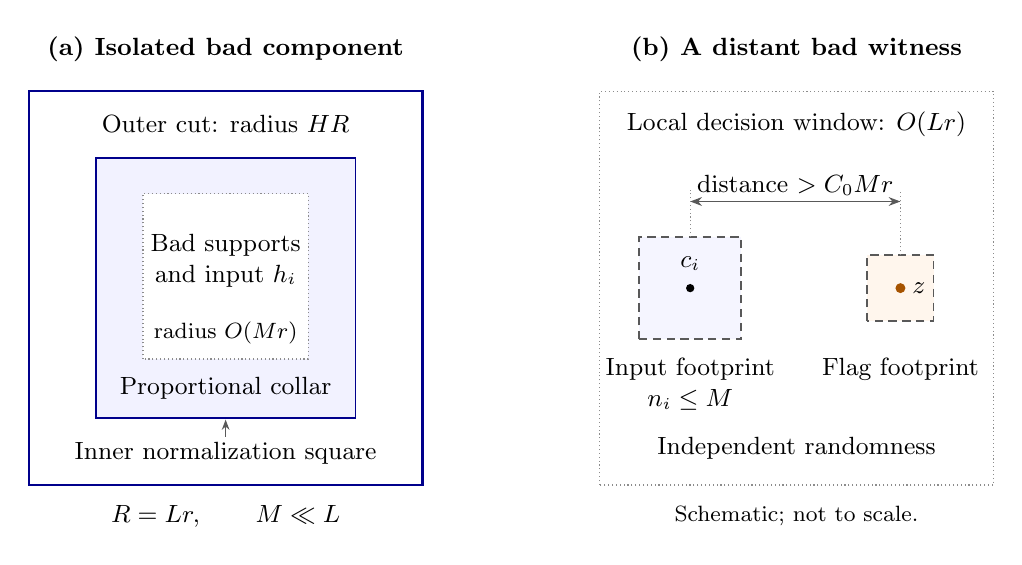
\begin{tikzpicture}[x=1cm,y=1cm,font=\small,
  outer/.style={draw=blue!55!black,line width=.8pt},
  inner/.style={draw=blue!55!black,line width=.65pt},
  footprint/.style={draw=black!65,densely dashed,line width=.65pt},
  guide/.style={draw=black!45,densely dotted},
  dimension/.style={draw=black!65,{Stealth[length=1.5mm]}-{Stealth[length=1.5mm]}}]
  \node[anchor=south,font=\small\bfseries] at (0,2.75)
    {(a) Isolated bad component};
  \draw[outer] (-2.5,-2.5) rectangle (2.5,2.5);
  \fill[blue!5] (-1.65,-1.65) rectangle (1.65,1.65);
  \fill[white] (-1.05,-.9) rectangle (1.05,1.2);
  \draw[inner] (-1.65,-1.65) rectangle (1.65,1.65);
  \draw[guide] (-1.05,-.9) rectangle (1.05,1.2);
  \node[align=center] at (0,.35) {Bad supports\\and input $h_i$};
  \node[font=\footnotesize] at (0,-.57) {radius $O(Mr)$};
  \node[fill=blue!5,inner sep=1.5pt] at (0,-1.27) {Proportional collar};
  \node[fill=white,inner sep=1.5pt] at (0,2.09)
    {Outer cut: radius $HR$};
  \node[fill=white,inner sep=1.5pt] at (0,-2.1)
    {Inner normalization square};
  \draw[black!65,-{Stealth[length=1.3mm]}] (0,-1.89) -- (0,-1.67);
  \node at (0,-2.90) {$R=Lr,\qquad M\ll L$};

  \begin{scope}[xshift=7.25cm]
    \node[anchor=south,font=\small\bfseries] at (0,2.75)
      {(b) A distant bad witness};
    \draw[guide] (-2.5,-2.5) rectangle (2.5,2.5);
    \node[fill=white,inner sep=1.5pt] at (0,2.08)
      {Local decision window: $O(Lr)$};
    \draw[footprint,fill=blue!4] (-2.0,-.65) rectangle (-.7,.65);
    \fill (-1.35,0) circle[radius=1.5pt];
    \node[anchor=south] at (-1.35,.1) {$c_i$};
    \node[anchor=north,align=center] at (-1.35,-.77)
      {Input footprint\\$n_i\le M$};
    \draw[footprint,fill=orange!7] (.90,-.42) rectangle (1.74,.42);
    \fill[orange!65!black] (1.32,0) circle[radius=1.8pt];
    \node[anchor=west,inner sep=1pt] at (1.43,0) {$z$};
    \node[anchor=north,align=center] at (1.32,-.77)
      {Flag footprint};
    \draw[dimension] (-1.35,1.1) -- (1.32,1.1)
      node[midway,above,inner sep=2pt] {distance $>C_0Mr$};
    \draw[guide] (-1.35,.65) -- (-1.35,1.25);
    \draw[guide] (1.32,.42) -- (1.32,1.25);
    \node[align=center] at (0,-2.04) {Independent randomness};
    \node[font=\footnotesize] at (0,-2.90) {Schematic; not to scale.};
  \end{scope}
\end{tikzpicture}
\caption{The two geometric mechanisms in the short-input estimate.
In (a), the supports of the bad fields and the short input lie in the
dotted square of radius $O(Mr)$.  The middle solid square provides a
proportional collar for pointwise
normalization of the positive bad weight before averaging to the
selected outer cut of radius $HR$.  The ratio of these radii produces
the $O(M/L)$ centered attenuation.  In (b), an exceptional short-input
contribution has a bad-center witness $z$ farther than $C_0Mr$ from
its anchor $c_i$, but within the local decision window of size
$O(Lr)$, where $C_0$ is the fixed witness-separation constant.
The separated footprints include the disorder and all
decision seeds, so the witness flag is independent of that input.
The panels illustrate separate cases; no particular arrangement of
bad fields or grid cells is prescribed.}
\label{norm:geometry}
\end{figure}


Long singletons, $n_i>M$, have a separate small factor.  Reserve an
input length weight after paying the output weight.  Their summed
majorant is at most
\begin{equation}\label{norm:long}
           \lambda_L=C L^C e^{-cM},
\end{equation}
times the relevant input norm.  The constants in the exponents depend
only on the already fixed weights and powers.  In particular $\lambda_L$
is smaller than every inverse power of $L$ as $L\to\infty$.
Finally, an analytic background term of order at least two is bounded
by $C_L\delta$ times a positive linear sum of input $X_i$: retain one
factor, bound all others by their good-field bounds, and sum the trees.
This observation holds in any probability measure, including a measure
weighted by a source.

\subsection{Reproduction of the background probability norms}
\begin{proposition}[High moments and recovery of $L^2$]\label{norm:reproduction}
Choose $L$ sufficiently large and then $\delta$ sufficiently small.
Under \eqref{norm:input},
\begin{align}
 \norm{h'}_{v,p}&\le Bs/8+C_L^*B_2s+o(s),\label{norm:high-reproduction}\\
 \norm{h'}_{v,2}&\le C_{\eta,L}F_*s+\eps_* Bs+o(s).
                                                    \label{norm:L2-reproduction}
\end{align}
Here $C_L^*$ grows at most polynomially in $L$.  For the second inequality,
assume that each output principal slot has diagonal second-moment
bound
\begin{equation}\label{norm:diagonal}
 \sup_\sigma\E|h'_a(\sigma)|^2\le e^{-2v}F_*^2s^2,
 \qquad F_*\ge1.
\end{equation}
A bound on its raw second tensor implies this hypothesis.  One can
choose $\eps_*<[100(1+C_L^*)]^{-1}$: first use the long-slot suppression,
then choose the dictionary accuracy $\eta$ and the mesh threshold $r_0$.
These choices do not depend on $B,B_2,F_*$.
\end{proposition}
\begin{proof}
For the first inequality, use the absolute decomposition just proved.
The nonlinear good terms cost $C_L\delta Bs$, and long singleton terms
cost $\lambda_LBs$.  A witness is independent of the short input it
multiplies.  Thus
\[
 \norm{X_i\one_{\mathcal B_c}}_p
  =\norm{X_i}_p\Prob(\mathcal B_c)^{1/p}
  \le C B^2\delta^{-1}s^2e^{-vn_i}.
\]
Minkowski's inequality and the finite witness sums give $O(s^2)$ at
fixed $L$.  It remains to estimate the attenuated short sum.

Expand its $p$th power.  Join two of the $p$ input anchors when their
distance is at most $C M$, choosing $C$ so that different components
have disjoint dependence carriers.  Call the connected components
bunches.  For a term with one bunch, choose the first anchor in at most
$CL^2$ ways.  A spanning tree on the $p$ labeled occurrences places
each successive anchor in at most $CM^2$ ways.  There are at most
$p^{p-2}$ such trees.  Animal shapes and slot lengths are summed with
the reserved weights.  Hence the count is at most $CL^2M^{C_p}$, and
\eqref{norm:product} bounds its expectation by $(Bs)^p$.  After taking
the $p$th root and including attenuation, this part costs
\begin{equation}\label{norm:one-bunch}
                 C L^{-1+2/p}M^{C_p} Bs.
\end{equation}

For two or more bunches, their random variables are independent.
Suppose a bunch contains $k<p$ occurrences.  H\"older within it uses
only $L^k$ norms.  For $2\le k<p$, interpolate by
\[
 \norm{X_i}_k\le\norm{X_i}_2^{\theta_k}
                   \norm{X_i}_p^{1-\theta_k},
 \qquad \theta_k=\frac{2(p-k)}{k(p-2)};
\]
for $k=1$ use $\norm{X_i}_1\le\norm{X_i}_2$.  The product of all
bunch estimates, after its $p$th root, is therefore
\[
 s B^{1-\theta}B_2^\theta
   \exp\{-v\textstyle\sum n_i/p\},\qquad \theta\ge1/p.
\]
For the last inequality, a singleton already contributes one to
$p\theta$.  If there are no singletons and there are $b\ge2$ bunches,
then $\sum k\theta_k=2p(b-1)/(p-2)\ge1$.  All placement
counts are polynomial in $L$: there are at most $p$ bunch roots, each
with $CL^2$ choices, followed by the preceding short-distance counts.
For each of the finitely many bunch patterns, weighted Young's
inequality gives, for any fixed $\varepsilon>0$,
\[
 C L^C B^{1-\theta}B_2^\theta
       \le\varepsilon B+C_{p,\varepsilon}L^{C_p}B_2.
\]
This also follows directly by maximizing the left side minus
$\varepsilon B$ as a function of $B/B_2$.  Since $1/\theta\le p$,
the resulting constant remains polynomial in $L$.  Sum over the
finitely many patterns.  Increase $L$ to make \eqref{norm:one-bunch}
and \eqref{norm:long} small; choose $\varepsilon$ for the multi-bunch
terms; then decrease $\delta$ for the nonlinear terms.  Allocating
less than $1/8$ in total to these coefficients of $B$ proves
\eqref{norm:high-reproduction}.

For the second inequality, first use \eqref{norm:quadratic-L2}.
The nonprincipal part of $Th$ has input length at least $L/2$, and its
$L^2$ norm is at most $CL^Ce^{-cL} Bs$.  A principal output of $Th$
has the form $\pi P_{HR}A$, where $A$ is the sum of the short-rule
inputs anchored in its parent cell and $\pi$ denotes plane centering.
All these inputs are supported in one inner square, separated by a
fixed proportional buffer from the $HR$ contour.  The weighted
placement bound and Minkowski give
\[
                     \norm{\norm A_\infty}_2\le C_L Bs.
\]
The finite dictionary of Lemma~\ref{ref:dictionary} supplies $N=N(\eta,L)$
actual contour assignments $\sigma_1,\ldots,\sigma_N$ such that
\[
 \norm{\pi P_{HR}A}_\infty
 \le \max_{\nu\le N}|\pi P_{HR}A(\sigma_\nu)|
                          +C\eta\norm A_\infty.
\]
This is a deterministic inequality and thus applies to the random $A$.
Replace each tested value of $Th$ by that of $h'$ using
\eqref{norm:quadratic-L2}.  The $L^2$ norm of the maximum of $N$ values
is at most the square root of the sum of their second moments.  By
\eqref{norm:diagonal}, after restoring the principal weight, this costs
$\sqrt N F_*s+O(s^2)$.  The net error costs $C_L\eta Bs$.
Choose $L$ so that the exponential long-slot coefficient is smaller
than the desired $\eps_*/2$; this is possible against the polynomial
$C_L^*$.  Then choose $\eta$ with $C_L\eta<\eps_*/2$ and increase
$r_0$ to the dictionary threshold.  This proves
\eqref{norm:L2-reproduction}.  Notice the order of the argument:
\eqref{norm:diagonal} is a tensor hypothesis, supplied later by the
Taylor flow, whereas the conclusion is a probability norm of a sup
norm.  They are not the same assertion.
\end{proof}

\subsection{Sources and mixed probability measures}
Let $u$ be a scaled singleton odd source list.  Put $Y_i=\norm{u_i}_\infty$
and suppose, for one of the chosen even $q$, that
\begin{align}
 (\E Y_i^q)^{1/q}&\le Ue^{-vn_i},\label{norm:source-input}\\
 (\E Y_i^qX_m^p)^{1/p}
  &\le U^{q/p}B_s s\,e^{-vq n_i/p-vn_m}.
                                      \label{norm:mixed-input}
\end{align}
The subscript on $B_s$ denotes ``source'': $B_s$ is a fixed constant,
whereas $U$ may change from one scale to the next.  No independence
between $u_i$ and a nearby $h_m$ is assumed.

\begin{proposition}[Source Taylor estimates and mixed reproduction]
\label{norm:source}
Under the preceding assumptions, moments with $q$ source occurrences
and at most two background arguments obey the ordinary Taylor rule
through total background degree two,
with error $O(U^qs^3)$ in the weighted projective norms.  Background
arguments already present in a tensor count toward that degree.
With fewer source arguments the corresponding bound follows by
H\"older.  Moreover,
\begin{equation}\label{norm:source-difference}
               \norm{u'-L^dTu}_{v,q}=O(Us),
\end{equation}
and the output satisfies
\begin{equation}\label{norm:mixed-output}
 \sup_{a,b}e^{vq n_a/p+vn_b}
       (\E\norm{u'_a}_\infty^q\norm{h'_b}_\infty^p)^{1/p}
 \le U^{q/p}\{B_s s/8+C_{L,B}s+o(s)\}.
\end{equation}
The choices of $p,L,\delta$ and the weights can be made before
$B_s$ and $U$.  All these estimates retain any saved scalar's carrier
until after its weighted estimate is taken.
\end{proposition}
\begin{proof}
For a fixed source input define the finite measure
$\dd\mu_i=Y_i^q\dd\Prob$.  Its mass is at most
$U^qe^{-vq n_i}$, and \eqref{norm:mixed-input} bounds the $p$th moment
of every $X_m$ in this measure.  Consequently, for nonnegative integers
$a_m$ of total $D\le p$,
\begin{equation}\label{norm:weighted-holder}
 \int\prod_m X_m^{a_m}\,\dd\mu_i
 \le U^q(B_s s)^D
       e^{-vq n_i-v\sum_m a_mn_m}.
\end{equation}
Indeed, apply H\"older with exponents $p/a_m$ and $p/(p-D)$, the last
factor being the mass of $\mu_i$.  The powers of $U$ and of the source
weight sum to exactly $q$.  A bad indicator supplies the unused
$p-D$ powers as in \eqref{norm:flagproduct}.

For $q$ possibly distinct source slots, H\"older first gives
\[
 \E\left[\prod_{\ell=1}^qY_{i_\ell}\prod_mX_m^{a_m}\right]
 \le\prod_{\ell=1}^q
       \left(\int\prod_mX_m^{a_m}\,\dd\mu_{i_\ell}\right)^{1/q}.
\]
Thus \eqref{norm:weighted-holder} retains decay in every source and
background index.  For fewer source occurrences include unweighted
probability measures in this H\"older step.  Apply this calculation to
the tree expansion, retaining three background factors in a remainder.
Additional good factors are bounded deterministically, and a changed
bad decision is paid by the unused mixed moment powers.  The same
summable series as in Proposition~\ref{norm:taylor} proves the asserted
$O(U^qs^3)$ bound.  In $L^q$ retain one background factor and use
\eqref{norm:weighted-holder} with degree $q$.  A bad flag costs
$O(Us^{p/q})$.  This proves \eqref{norm:source-difference}, since
$p/q>1$.

We give the high mixed estimate separately.  Normalized tilted
conditional moments and the deterministic good-field bounds imply a
positive linear majorant
\begin{equation}\label{norm:source-majorant}
             Y'_a\le\sum_i K_{ai}Y_i,\qquad K_{ai}\ge0.
\end{equation}
Here the coefficients are deterministic majorants, not the realized
coefficients of the map.  They include the factor $L^d$.  Lemma
\ref{block:tree}, with the source vertex retained, proves that their
weighted row sums are bounded by $C L^d$; reserving additional input
length weight makes the part with $n_i>M$ bounded by
$CL^Ce^{-cM}$.  These statements mean row sums after paying the
requested output weight from the input weight; they also hold with
all the fractional weights appearing below.  In particular no factor
$\norm{\log P e^B}$ occurs in \eqref{norm:source-majorant}.
To construct $K_{ai}$, sum the absolute tree majorants over the allowed
carrier and anchor assignments, taking the prescribed enlarged union
of input carriers for each output.  Every realized routing is one of
these boundedly many assignments.  There is no sum over patterns of
threshold outcomes or over the amplitudes of bad fields.

Fix output background slot $b$ and source input $i$.  Estimate
$\norm{\norm{h'_b}_\infty}_{L^p(\mu_i)}$ using the deterministic
decomposition preceding Proposition~\ref{norm:reproduction}.  If
$n_i>M$, crude Minkowski and \eqref{norm:mixed-input} give
\begin{equation}\label{norm:mixed-long-source}
 \norm{\norm{h'_b}_\infty}_{L^p(\mu_i)}
 \le C_L U^{q/p}B_s s\,e^{-vq n_i/p-vn_b}.
\end{equation}
There is still a reserved exponential in $n_i$ for its subsequent
source sum.

Suppose now $n_i\le M$.  Long background inputs and nonlinear good
terms cost, respectively, $\lambda_L B_s s$ and $C_L\delta B_s s$,
times the common factor $U^{q/p}e^{-vq n_i/p-vn_b}$.
For short background inputs with anchors within $10M$ of the source
anchor, use \eqref{norm:mixed-input}.  There are at most $CM^2$
anchors.  Animal lengths and shapes cost a constant after their weight
sums.  The attenuated part of \eqref{norm:witness-bound}, estimated
by Minkowski, therefore costs
\[
       C M^C L^{-1} B_s s\,
                  U^{q/p}e^{-vq n_i/p-vn_b}.
\]
For its witness part the witness carrier is disjoint from the union
of the source and background input carriers.  Exact independence gives
\[
 \big(\E Y_i^q X_m^p\one_{\mathcal B_c}\big)^{1/p}
   =\big(\E Y_i^qX_m^p\big)^{1/p}\Prob(\mathcal B_c)^{1/p},
\]
so this part gains an additional factor $O(Bs/\delta)$ and is
$O(U^{q/p}s^2)$ at fixed constants.  For short background anchors
farther than $10M$, the background input is independent of $Y_i$.
Drop any witness indicator and use
\[
 \big(\E Y_i^qX_m^p\big)^{1/p}
       = (\E Y_i^q)^{1/p}(\E X_m^p)^{1/p}
       \le U^{q/p} Bs\,e^{-vq n_i/p-vn_m}.
\]
Even a crude sum over these anchors has only a polynomial cost in $L$.
Combining these estimates gives, for short $i$,
\begin{equation}\label{norm:mixed-fixed-source}
 \norm{\norm{h'_b}_\infty}_{L^p(\mu_i)}
 \le U^{q/p}e^{-vq n_i/p-vn_b}
       \{a_LB_s s+C_LBs+o(s)\},
 \quad a_L=C M^C/L+\lambda_L+C_L\delta.
\end{equation}

We now check the powers when summing sources.  Put
$F_i=(\E Y_i^q\norm{h'_b}_\infty^p)^{1/p}$.
Minkowski in $L^q$, applied to \eqref{norm:source-majorant}, yields
\begin{equation}\label{norm:mixed-minkowski}
 (\E (Y'_a)^q\norm{h'_b}_\infty^p)^{1/p}
             \le \left(\sum_i K_{ai}F_i^{p/q}\right)^{q/p}.
\end{equation}
This is an $\ell^{p/q}$ norm with weights $K_{ai}$.  Apply its triangle
inequality to the three terms in braces in
\eqref{norm:mixed-fixed-source}.  Raising the input source weight to
$p/q$ gives $(e^{-vq n_i/p})^{p/q}=e^{-vn_i}$, exactly the weight needed in
the positive source sum.  The background output weight remains
$e^{-vn_b}$ after taking the power $q/p$.  Hence the short-source
coefficient of $B_s s$ is at most
\[
          (CL^d)^{q/p}\big(CM^C/L+\lambda_L+C_L\delta\big),
\]
whereas the far-background term is a constant $C_{L,B}s$ independent
of $B_s$.  For the long-source part use
\eqref{norm:mixed-long-source} and the reserved exponential in its
row sum; its coefficient is at most $CL^Ce^{-cM q/p}$.
First choose $L$ large.  Since $dq/p<1$ and $M$ is a power of $\log L$,
the first attenuation coefficient tends to zero, as do both long
coefficients.  Then choose $\delta$ small.  Their sum can be made less
than $1/8$.  Witness errors have an extra positive power of $s$ and
remain $o(s)$ after \eqref{norm:mixed-minkowski}, whose use of the
$\ell^{p/q}$ triangle inequality is homogeneous of degree one in $F_i$.
This proves \eqref{norm:mixed-output}.
\end{proof}

The deterministic estimate \eqref{norm:source-majorant} also explains
why marked readout is possible in boxes whose principal background
fields are large near the boundary.  Before any probability estimate,
the homogeneous transport of a coefficient with a fixed set of mark
labels has a bounded weighted operator cost per step, with the
prescribed factors $L^d$ for its marks.  A freshly generated coefficient
with two distinct marks has a bounded bilinear cost in the two singleton
lists and retains both carriers and its saved scalar carrier; apply
Lemma~\ref{block:tree} with two source vertices.
A background factor retained at a merge can then be estimated under
the source-weighted measures above, even when the two sources are
correlated with it.  No large-field logarithm multiplies either source.

We finish by making the dependence of choices explicit.  Fix the
source powers, then $p$, the finite collection of weights and their
counting slack, and the geometric halos.  Choose $L$ for attenuation,
long-slot compression and the one-bunch bound.  Choose $\delta$ for
convergence and the small nonlinear coefficients.  The polynomial
$C_L^*$ is now fixed.  Choose $\eps_*$, dictionary accuracy $\eta$, and
$r_0$ in that order.  The moment constants $B_2,B,B_s$ and the tensor
allowances may then be fixed, and finally $s$ made sufficiently small.
In particular an allowance depending on the starting mesh does not
force a new mesh choice.  Because every contraction above has fixed
slack, the same inequalities hold on replacing the next-scale targets
$s,U$ by $s(1+O(s^2))$ and $U(1+O(s))$, respectively.  The stronger
variation $U(1+O(s^2))$ used after the marked cumulant comparison is
therefore covered as well.

\section{Linear transport and its distinguished coordinates}\label{sec:linear}
The Taylor estimates of Section~\ref{sec:norms} reduce the background flow to
its first four cumulant arrays.  We now identify the directions which linear
blocking does not contract.  There is one expanding mean direction and one
neutral covariance direction.  A spin insertion has one neutral direction
after multiplication by the scale factor $L^d$.  The distinction between a
covariance per unit area and a homogeneous perturbation is essential here.

\subsection{Coordinates and exact representatives}
Write $a(i)$ for the anchor cell of a slot $i\in \mathcal I_r$.  The array spaces and
indexed projective norms are those of Section~\ref{sec:blocking}: the tensor
norm at fixed indices is the projective tensor norm of the function sup norms,
and the array weight is $e^{v\sum n_i}$.  All unmarked arrays in this section
are invariant under grid translations and square symmetries.  A connected
array is zero unless the safety adjacency graph of its dependence carriers
is connected.  This is the support condition satisfied by joint cumulants of
the random lists.  Whenever indices are summed, an unused part of the
exponential weight pays the animal counts and polynomial size factors.

Let $\ell$ and $\ell_s$ be the charges of Lemma~\ref{ref:charges}.
For an even function and a scaled odd function, respectively, put
\[
 q_r(F)=r^{-1}\ell(F),\qquad q_{r,s}(U)=r^{-d}\ell_s(U).
\]
These are bounded functionals on a slot of length $n$, with norms at most
$C(n+S)$ and $C(n+S)^d$.  For a homogeneous mean array $m$ and a homogeneous
connected two-tensor $K$, define
\begin{align}
 x_r(m)&=\sum_{a(i)=c}q_r(m_i),\label{lin:x}\\
 g_r(K)&=\sum_{a(i)=c}\sum_{k\in \mathcal I_r}
                  (q_r\otimes q_r)(K_{i,k}).\label{lin:g}
\end{align}
The values do not depend on the cell $c$.  The second sum converges absolutely:
connectivity puts the second anchor within $C(n_i+n_k+S)r$ of the first,
and exponential weights dominate this number of placements.  The factor
$r^{-2}$ in~\eqref{lin:g} divides the charge covariance by the number of
microscopic sites in one cell.  Thus $g_r$ is a variance density.

Let $P_{Hr,c}$ denote reference conditional averaging to the square contour
with radius $Hr$ about the center of $c$, followed, for even functions, by
plane centering.  Define arrays supported on principal slots by
\begin{align}
 (v_j)_{p_c}&=r_j^{-1}\sum_{z\in c}P_{Hr_j,c}e(z),
       &x_{r_j}(v_j)&=1,\label{lin:v}\\
 (V_j)_{p_c,p_c}&=\sum_{z\in c}
                       \bigl(P_{Hr_j,c}e(z)\bigr)^{\otimes2},
       &g_{r_j}(V_j)&=1.\label{lin:V}
\end{align}
All other entries of $V_j$ vanish.  The charge identities follow from
$\ell(e(z))=1$ and $|c|=r_j^2$.  The bounds
$\|P_{Hr_j,c}e(z)\|\le C/r_j$ show that both representatives have uniformly
bounded indexed norms, including the projective norm of $V_j$.

Write $T_j$ for linear background transport and $T_j^{(k)}$ for its induced
transport on $k$-tensors, including the prescribed reindexing and sums.
Nested contours and the tower property give the exact identities
\begin{equation}\label{lin:exact}
 T_jv_j=Lv_{j+1},\qquad T_j^{(2)}V_j=V_{j+1},\qquad
 x_{r_{j+1}}T_j=Lx_{r_j},\qquad
 g_{r_{j+1}}T_j^{(2)}=g_{r_j}.
\end{equation}
For example, the $L^2$ child cells partition a parent cell, so transporting
\eqref{lin:v} yields
\[
 r_j^{-1}\sum_{z\in c'}P_{Hr_{j+1},c'}e(z).
\]
For~\eqref{lin:V}, each microscopic diagonal tensor is transported to the
same parent contour in both factors.  No off-diagonal microscopic pair is
created.  These observations also explain why the two multipliers differ.
The coordinate identities follow by preserving charges and dividing by
$R$ or $R^2$, respectively.  Reindexing long slots preserves the same total
charge sums.  We use the bounded projections
\[
 \Pi_{m,j}m=x_{r_j}(m)v_j,\qquad
 \Pi_{K,j}K=g_{r_j}(K)V_j.
\]

\begin{proposition}[Background linear splitting]\label{lin:background}
Fix the finite set of weights needed in Section~\ref{sec:norms}.  By taking
$L$ sufficiently large, all the following contraction constants can be made
smaller than any prescribed $\kappa>0$:
\[
 \|T_jm\|\le\kappa\|m\|\quad(x_{r_j}(m)=0),\qquad
 \|T_j^{(2)}K\|\le\kappa\|K\|\quad(g_{r_j}(K)=0),
\]
and $\|T_j^{(k)}A\|\le\kappa\|A\|$ for homogeneous connected arrays of
orders $k=3,4$.  Norms here and below have the fixed input and output weights
allocated to the corresponding estimate.  The bounds are uniform in $j$.
The two projections above intertwine transport with multipliers $L$ and $1$.
\end{proposition}

\begin{proof}
Put $M=(\log L)^3$.  If an input length exceeds $M$, the unused exponential
weight gives $C L^C e^{-cM}$ after all linear placement sums.  Charge
projection adds only polynomial factors in the lengths.  Consequently these
long inputs, including the charge needed to compensate their removal, have
norm at most $\eta_L\|A\|$, where $\eta_L\to0$ faster than every fixed
negative power of $L$.  It suffices to estimate the inputs of lengths at
most $M$; constants denoted by $C M^C$ include their weighted index sums.

For the mean, collect all short slots with anchor $c$ into one even
function supported in a square of radius $C M r$.  Homogeneity and square
symmetry make this grouped function square symmetric about $c$.  Its charge
is zero, up to the discarded long-input charge.  Subtract that charge using
a translated copy of $v_j$ before applying the reference estimate.  The
square-symmetric charge-zero exponent is $3-\nu$, so one child contribution
at the parent contour costs $C M^C L^{-3+\nu}$.  There are $L^2$ child
anchors.  Thus the short part is bounded by
$C M^C L^{-1+\nu}\|m\|$, plus $\eta_L\|m\|$ for the compensation.
The grouped function is formed before taking its sup norm; the triangle
inequality and the weighted slot sum bound that norm by the input array
norm.  This is where the square symmetry of the law is used.

For the covariance, connectivity and the short-length restriction put the
two anchors within $C M r$ of one another.  Separate pairs whose anchors go
to different parent cells from pairs going to the same parent.  In the first
case, an anchor lies in a strip of width $C M r$ about the boundary of a
parent cell.  There are $C L M$ such fine cells per parent.  Each centered
factor costs at most $C M/L$ under averaging; after the weighted sums over
slot shapes and the other anchor, this contribution is at most
\begin{equation}\label{lin:strip}
 C M^C L^{-1}\|K\|.
\end{equation}
This bound applies also to pairs inside one parent for which the first anchor
lies in that strip.

For the remaining pairs work first with one elementary projective tensor
$F\otimes G$.  If $c$ is its first anchor and $z_c$ the center site of $c$,
replace both factors by their charges times the same unit-charge field:
\[
 F\longmapsto q_r(F)\,rP_{Hr,c}e(z_c),\qquad
 G\longmapsto q_r(G)\,rP_{Hr,c}e(z_c).
\]
Their supports and the original supports are contained in a square of
radius $C M r$.  After subtracting the charge, the even improved estimate
and the tower property bound a replaced-factor error at the parent contour
by $C M^C L^{-2+\nu}$ times the original factor norm.  The other factor has
its usual $C M^C/L$ bound.  Summing $L^2$ first anchors gives
$C M^C L^{-1+\nu}\|K\|$ for terms containing a replacement error.

It remains to sum the term in which both factors were replaced.  With the
first anchor fixed, the transported elementary pair is the same for every
choice of its second slot or anchor.  Its scalar coefficient is therefore
the corresponding sum in~\eqref{lin:g}, and vanishes on the kernel of $g_r$.
For an anchor outside the strip, every short connected second anchor goes
to the same parent, so this cancellation is complete.  Restriction to short
inputs leaves only the discarded long-input charge, already bounded by
$\eta_L$.  Strip anchors were estimated in~\eqref{lin:strip}.  Homogeneity
is needed here to make the zero coordinate condition hold at every first
anchor; it is not a statement about an arbitrary nonhomogeneous covariance.
Taking infima over projective decompositions proves the asserted tensor
bound without any factor depending on the dimension of the function spaces.

Finally, a connected short $k$-tuple has all its anchors within $C_k M r$
of its first anchor.  The first anchor has $C L^2$ possible positions in a
rooted parent cell, and each of the $k$ centered factors costs $C M/L$.
Weighted sums bound the result by $C M^C L^{2-k}\|A\|$ for $k=3,4$.
Together with the long part and the preceding estimates this tends to zero.
The intertwining assertions follow from~\eqref{lin:exact}.
\end{proof}

\subsection{One marked point and tensor copies}
For a fixed marked site $y$, let $c_j(y)$ be its cell and put
\begin{equation}\label{lin:w}
 (w_{j,y})_{p_{c_j(y)}}=r_j^dP_{Hr_j,c_j(y)}\sigma_y.
\end{equation}
This is an odd scaled source list, with all other entries zero.  Its total
normalized spin charge is one.  For an arbitrary marked list $u$, and for
an array of $q$ marked copies whose slot indices are kept separate, set
\[
 Q_{j,y}(u)=\sum_i q_{r_j,s}(u_i),\qquad
 Q_{j,q,y}(U)=\sum_{i_1,\ldots,i_q}
                   q_{r_j,s}^{\otimes q}(U_{i_1,\ldots,i_q}).
\]
Every marked carrier contains $y$, so these are bounded functionals in the
weighted indexed spaces.  Write $\mathcal T_j=L^dT_j$ for scaled odd
transport and $\mathcal T_j^{(q)}$ for its tensor extension.  The exact
identities are
\[
 \mathcal T_jw_{j,y}=w_{j+1,y},\qquad
 Q_{j+1,q,y}\mathcal T_j^{(q)}=Q_{j,q,y}.
\]
The corresponding projection is
$\Pi_{q,j,y}U=Q_{j,q,y}(U)w_{j,y}^{\otimes q}$.

\begin{proposition}[Marked linear splitting]\label{lin:marked}
For each fixed finite set of positive integers $q$, the operators
$\mathcal T_j^{(q)}$ are bounded uniformly in $j,y,L$.  On
$\ker Q_{j,q,y}$ their norms tend to zero as $L\to\infty$.
A connected array comprising this marked tensor as one grouped argument and
at least one even background argument contracts without removal of a line.
The one-source kernel estimate also holds pathwise, and hence in each of the
weighted random-list $L^p$ norms used in Section~\ref{sec:norms}.
\end{proposition}

\begin{proof}
For a short source slot the ordinary odd estimate gives
$C((n+S)/L)^d$ before source scaling.  Multiplication by $L^d$ and summation
with the unused exponential weight give a constant independent of $L$;
one sums $(n+S)^d$ against that weight, rather than replacing it by $M^d$.
Long slots are again bounded by $C L^C e^{-cM}$.

For each short slot individually, subtract its normalized charge times the
representative at its input scale.  Both functions fit in a square of radius
$C(n+S)r$ containing $y$.  The charge-zero odd estimate, whose exponent is
$1+d-\nu$, followed by source scaling, bounds the difference between the
transported slot and its charged representative by
$C(n+S)^C L^{-1+\nu}$ times its norm.  Summing over slots is legitimate by
the exponential weights.  Long slots admit the same subtraction with a
beyond-polynomially small bound, since charge extraction has only a
polynomial size cost.  This gives a componentwise decomposition into a
bounded rank-one map and a remainder of arbitrarily small norm.

Apply that decomposition separately to each factor of an elementary
projective $q$-tensor.  The all-line term is exactly
$Q_{j,q,y}(U)w_{j+1,y}^{\otimes q}$.  Every other term contains a small
remainder and at most $q-1$ bounded factors.  The sum of its $2^q-1$ choices
is small for fixed $q$.  Infimizing over decompositions proves the result
in the projective norm.  In particular no norm comparison involving the
number of spin configurations is used.

A connected array with an additional background factor has no $L^2$ volume
sum: its root is the fixed mark.  Connectivity bounds the remaining anchor
sums by powers of the slot lengths.  At least one even factor supplies
$C M^C/L$, whereas the scaled marked factors stay bounded.  This proves
contraction in the mixed sector.  All these are componentwise deterministic
inequalities, so applying the center-coordinate projection to each random
realization and then taking its $L^p$ norm gives the last assertion.  The
buffer $H$ keeps every point of a cell uniformly away from its cutting
contour, making the constants independent of the position of $y$ in its
cell.
\end{proof}

\section{The marginal coefficients from finite insertions}\label{sec:coefficients}
Linear transport leaves the variance density unchanged.  Its first nonlinear
increment, and the first increments of marked charge moments, must therefore
be computed.  We compute their averages over scales by comparing linear
charges of logarithms with normalized charges of finite products of
microscopic insertions.  The latter charges are preserved by the exact
partition identities.  Only coefficients through degree four are used;
there is no infinite-volume random power series in this argument.

\subsection{A bounded-degree test and its profiles}
Give every microscopic site $i$ a formal variable $t_i$ and start with the
factor $1+t_i e(i)$.  Initially its logarithm is put into the principal slot
of its cell.  First work with finitely many sites and retain only the degrees
needed below.  Apply the ordinary Taylor rules at the zero background, and
then substitute
\begin{equation}\label{coef:test}
 t_i=\lambda\eta_i,\qquad
 \Prob(\eta_i=1)=\Prob(\eta_i=-1)=\tfrac12,
\end{equation}
with independent signs.  Coefficient notation $[\lambda^k]$ means the
coefficient, without a factorial.  At fixed degree and fixed scale every
coefficient has bounded range.  A large finite window may consequently tend
to the whole plane after that coefficient has been computed.  Averaging over
the signs gives homogeneous arrays in the norms of Section~\ref{sec:linear}.
For a mark at $y$ start with $r_0^d\sigma_y$ and use scaled marked transport.

Let $h_j$ be the formal background list and $u_{j,y}$ its scaled marked
list.  Define
\begin{align*}
 m_j^*&=[\lambda^2]\E h_j,&
 K_j^*&=[\lambda^2]\Cov(h_j,h_j),\\
 W_j^*&=[\lambda^4]\cum(h_j,h_j,h_j),&
 Y_j^*&=[\lambda^4]\cum(h_j,h_j,h_j,h_j).
\end{align*}
For a fixed positive integer $q$ the $q$ source indices remain separate in
$u_{j,y}^{\otimes q}$, but that tensor is one grouped random argument in the
joint cumulant
\begin{equation}\label{coef:Z}
 Z_{j,q,y}^*=[\lambda^2]\cum(u_{j,y}^{\otimes q},h_j).
\end{equation}
Put
\begin{align}
 \beta_j&=[\lambda^4]g_{r_j}\bigl(\Cov(h_j,h_j)\bigr),
       &b_j&=\beta_{j+1}-\beta_j,\label{coef:b}\\
 \alpha_{j,q}(y)&=[\lambda^2]\E
                   Q_{j,q,y}(u_{j,y}^{\otimes q}),
       &c_{j,q}(y)&=\alpha_{j+1,q}(y)-\alpha_{j,q}(y).
       \label{coef:c}
\end{align}
The definitions include any bounded initial-scale discrepancy between a
microscopic list and the averaged representatives of Section~\ref{sec:linear}.

\begin{lemma}[Uniform formal profiles]\label{coef:profiles}
For $j\ge1$, the arrays $m_j^*,W_j^*,Y_j^*,Z_{j,q,y}^*$ have bounded indexed
projective norms, uniformly in $j$ and $y$ and for every fixed finite set of
$q$'s.  Moreover $K_j^*=V_j$ and the degree-zero marked list is $w_{j,y}$.
The coefficients $b_j$ and $c_{j,q}(y)$ are uniformly bounded.
\end{lemma}

\begin{proof}
Linear insertions propagate by nested averaging.  Thus the coefficient of
$t_i$ at scale $r$ is $P_{Hr,c(i)}e(i)$ in the principal slot of its current
cell, giving $K_j^*=V_j$ exactly, and the same statement for the spin gives
$w_{j,y}$.  We explain separately why the mean profile stays bounded despite
the expanding mean direction.

For one microscopic variable, write $H_{i,k}^{(j)}$ for its $t_i^k$ coefficient
in the plane-centered background log list at scale $j$.  All its anchors
follow the same chain of parent cells.  The fixed-degree carrier estimate
of Lemma~\ref{block:carrier} bounds the number of occupied slot types
and their lengths by constants independent of $j$.  Increasing $L$ makes
these slots short for linear transport.  Constants in the present formal
calculation may depend on $L$ and $r_0$.  We claim
\begin{equation}\label{coef:single-columns}
 \|H_{i,1}^{(j)}\|\le Cr_j^{-1},\qquad
 \|H_{i,2}^{(j)}\|\le Cr_j^{-2}.
\end{equation}
The first bound is the reference energy estimate.  At a step from radius
$s$ to $Ls$, every freshly generated quadratic term costs $C\|H_{i,1}\|^2$,
hence at most $C_L(Ls)^{-2}$.  To bound the transported old quadratic terms,
condition on one contour outside all earlier cuts.  The exact identity,
with saved constants restored, represents the original factor $1+t_i e(i)$.
Its quadratic coefficient is zero.  Its first scalar coefficient is zero
because $e(i)$ is plane centered.  Equating quadratic coefficients therefore
gives, modulo constants,
\begin{equation}\label{coef:single-cancel}
 P H_{i,2}=-\tfrac12 P(H_{i,1}^2).
\end{equation}
Here each $H$ denotes the sum of its list entries before this common outer
average.  The linear rule puts these old short entries in the same parent
principal slot; cancellation in~\eqref{coef:single-cancel} thus occurs
before taking its norm.  The right side is bounded by $C s^{-2}$.
Combining old and fresh terms proves the second bound at the next scale.
At the first scale the bound is included by the allowed constant depending
on $L,r_0$.  This reasoning also covers earlier saved scalar coefficients:
they are reinstated for the exact identity and disappear upon plane
centering.  Their footprints obey the same carrier bound.

Only squares of individual signs contribute to $[\lambda^2]\E h_j$.
There are at most $C r_j^2$ microscopic sites which can contribute to a fixed
output anchor.  Summing the second estimate in~\eqref{coef:single-columns}
proves the bound on $m_j^*$.  The finitely many fixed-degree slot lengths
permit the same conclusion with the indexed exponential weights.

For completeness, the remaining profile recurrences follow by the
moment--cumulant partition formula.  The lowest nonzero fourth-cumulant
coefficient has four linear background letters, so $Y_j^*$ transports
homogeneously by $T_j^{(4)}$.  At degree four the third cumulant has, besides
its homogeneous term, only a quadratic output letter and two linear output
letters.  Its input partitions use either $Y_j^*$ or two copies of $V_j$.
These terms are bounded by the multilinear estimates of
Proposition~\ref{norm:taylor}.  The strict contractions of
Proposition~\ref{lin:background} therefore bound $Y_j^*$ and $W_j^*$.
In~\eqref{coef:Z}, the constant marked tensor is deterministic.  Its first
nonzero covariance with a background uses one linear marked correction and
one linear background letter.  The recurrence is the contracting connected
marked/background transport, with bounded forcing from the constant marked
tensor and $V_j$; hence $Z_{j,q,y}^*$ is bounded by
Proposition~\ref{lin:marked}.  The degree-two coefficient of
$\cum(u_{j,y}^{\otimes q},h_j,h_j)$ is zero: at that degree the marked
argument is deterministic, and a joint cumulant with a deterministic
argument vanishes.

Finally, in the degree-four covariance increment the linearly transported
covariance has identical $g$ coordinate.  The remaining partitions use
$W_j^*,Y_j^*,V_j\otimes V_j$, or $m_j^*\otimes V_j$, all bounded.  In the
degree-two marked-charge increment the transported marked tensor likewise
has unchanged charge; the remaining terms use $m_j^*,V_j$ and
$Z_{j,q,y}^*$, while the connected two-background profile just discussed
vanishes.  This proves the asserted bounds on the increments.
\end{proof}

\subsection{Charges invariant under a finite sequence of cuts}
For finitely many microscopic insertions let $H_*^{(j)}$ be the sum of the
plane-centered log-list entries produced through scale $j$.  At any fixed
coefficient order this is a finite sum with its full carrier footprints.
Let $f_i^{(j)}$ be the unscaled coefficient of one square-free spin source
in log-list slot $i$, and set $f^{(j)}=\sum_i f_i^{(j)}$.  The scaled
source entries are $u_{j,i}=r_j^d f_i^{(j)}$.  In particular,
\[
 Q_{j,q,y}(u_j^{\otimes q})=\ell_s(f^{(j)})^q.
\]
This identity connects the scalar charge calculation below to the indexed
tensor coordinate in~\eqref{coef:c}.  Define formal normalized charges by
\begin{equation}\label{coef:invariants}
 \mathcal E_j=\frac{\ell(\exp H_*^{(j)})}
                    {\langle\exp H_*^{(j)}\rangle_0},\qquad
 \mathcal S_j=\frac{\ell_s(f^{(j)}\exp H_*^{(j)})}
                    {\langle\exp H_*^{(j)}\rangle_0}.
\end{equation}
Both denominators have constant term one, so their formal reciprocals are
well defined.  Saved background constants cancel between numerator and
denominator.  A saved odd scalar is zero by spin-flip symmetry.

\begin{lemma}[Finite-insertion invariance]\label{coef:invariance}
Each coefficient of $\mathcal E_j$ and $\mathcal S_j$ in the formal variables
is independent of $j$.  It equals the corresponding normalized charge of
the original microscopic product and, for $\mathcal S_j$, its spin insertion.
\end{lemma}

\begin{proof}
Fix the coefficient and place an outer contour beyond every cut and carrier
which occurs in it.  For each fixed spin assignment on that contour, apply
Proposition~\ref{block:exact} to the system inside it.  The termwise
conditional-expectation proof of that proposition leaves these contour spins
fixed: each inner cut is an application of the tower property within this
conditional reference measure.  Thus the conditional partition expression,
as a function of the outer spin assignment, agrees before and after every
step.  Its source derivative gives the analogous identity with the single
odd insertion.  Let $C_j$ be the saved scalar formal series, so that the restored
weight is $e^{C_j}\exp H_*^{(j)}$.  Taking the reference plane average
proves that $e^{C_j}\langle\exp H_*^{(j)}\rangle_0$ is independent
of $j$.  Taking the disk-response limit defining $\ell$ or $\ell_s$
proves the corresponding invariance of each charge numerator multiplied
by $e^{C_j}$.  The saved scalar with one odd source is zero, so the marked
identity has this same scalar factor.  Every operation involves a finite
coefficient and finitely many cuts; no interchange with a convergent
infinite formal expansion is involved.  Dividing cancels $e^{C_j}$ and
proves the claim.
\end{proof}

We next quantify the difference between these invariant charges and the
linear charges $\ell(H_*^{(j)})$ and $\ell_s(f^{(j)})$ which occur in the
Taylor coordinates.  In the following bounds set $r=r_j$ and
$h=1+|i-k|$ for two distinct sites.  For $h\le Cr$ we have
\begin{equation}\label{coef:mixed-column}
 \|[t_it_k]H_*^{(j)}\|\le \frac{C}{hr}.
\end{equation}
The norm here is the sum of the finitely many occupied slot norms, with
fixed-degree weights; it also bounds their aggregate sup norm.  A mixed
coefficient cannot be generated before the two microscopic descendants have
contacting carriers.  This requires a generation radius $s\ge c_Lh$.
At radius $s$ a new quadratic coefficient costs $C_Ls^{-2}$.
Subsequent linear transport along ancestor cells is nested conditional
averaging and has centered-even bound $C_Ls/r$.  Anchor splitting adds only
a fixed-degree number of terms, already included in the constant.  Thus
\[
 \sum_{\substack{s=r_b\le r\\s\ge c_Lh}}
       C_Ls^{-2}\frac{s}{r}
 \le \frac{C_L}{r}\sum_{b:r_b\ge c_Lh}r_b^{-1}
 \le \frac{C_L}{hr}.
\]
This also covers $h$ below the starting radius by changing the constant.
The last generation has no further averaging and obeys the same bound.

For one energy site and one spin mark, put $h=1+|i-y|$.  The corresponding
bounds are
\begin{equation}\label{coef:marked-columns}
 \|[1]f^{(j)}\|\le Cr^{-d},\qquad
 \|[t_i]f^{(j)}\|\le Cr^{-d}h^{-1}.
\end{equation}
Indeed a mixed spin/energy generation at radius $s\ge c_Lh$ costs
$C_Ls^{-1-d}$ and subsequent odd averaging costs $C_L(s/r)^d$.
The geometric sum is $C_Lr^{-d}\sum_{b:r_b\ge c_Lh}r_b^{-1}$, as claimed.
All supports in these comparisons fit in a square of radius $C_Lr$.
Charge extraction therefore costs at most $C_Lr$ for even functions and
$C_Lr^d$ for odd functions.

\subsection{The covariance increment}
\begin{proposition}[Averages of the marginal coefficients]\label{coef:averages}
The coefficients in~\eqref{coef:b}--\eqref{coef:c} satisfy
\begin{align}
 \sum_{j<J}b_j&=-4\pi a^2\log r_J+o(\log r_J),\label{coef:bsum}\\
 \sum_{j<J}c_{j,q}(y)&=\binom q2\frac{\pi a^2}{2}\log r_J
                         +o(\log r_J),\label{coef:csum}
\end{align}
where the second error is uniform in $y$ for each fixed $q$.  Equivalently,
their Ces\`aro means are $-4\pi a^2\log L$ and
$\binom q2(\pi a^2/2)\log L$.
\end{proposition}

\begin{proof}
We first prove~\eqref{coef:bsum}.  The coordinate $\beta_J$ is the
coefficient of degree four in the variance per unit microscopic area of
$\ell(H_*^{(J)})$.  To see this directly, restrict to a large union of cells,
sum its linear charges, divide its variance by the number of microscopic
sites, and let the window grow.  At fixed $J$ the coefficient arrays have
bounded range, so the boundary contribution vanishes.  Formula~\eqref{lin:g}
is precisely the resulting anchored covariance sum.  At degree four,
averaging the independent signs leaves only one-site terms and unordered
two-site terms.  Terms supported on disjoint noninteracting insertions
cancel in the variance subtraction.  The surviving pair separations are
at most $C_Lr_J$, by the fixed-degree carrier bound.

Fix two sites $i\ne k$ and abbreviate
\[
 C_{ik}=\langle e(i)e(k)\rangle_0,\qquad
 A_{ik}=\ell(e(i)e(k)).
\]
Their invariant energy charge is exactly
\begin{equation}\label{coef:pair-rational}
 \mathcal E=
 \frac{t_i+t_k+A_{ik}t_it_k}{1+C_{ik}t_it_k}.
\end{equation}
The numerator uses $\ell(e(i))=\ell(e(k))=1$ and $\ell(1)=0$;
the denominator uses the centering of each energy.  Through degree three,
\begin{equation}\label{coef:pair-expansion}
 \mathcal E=t_i+t_k+A_{ik}t_it_k
              -C_{ik}(t_i^2t_k+t_it_k^2)+O(t^4).
\end{equation}
Here $O(t^4)$ denotes only discarded formal monomials of total degree at
least four.  Consequently the degree-four variance contribution after
$t_i=\lambda\eta_i$, $t_k=\lambda\eta_k$ is
\begin{equation}\label{coef:pair-value}
 A_{ik}^2-4C_{ik}.
\end{equation}
The square of the quadratic mixed term supplies $A_{ik}^2$; its mean is
zero.  The two linear/cubic crosses each supply $-2C_{ik}$.
Pure quadratic terms, if present in a different log representation, are
deterministic after the sign substitution and disappear in the variance.

We justify replacing the linear charge by this invariant charge with a
bounded total error.  Write $A_i=[t_i]H_*$, $B_i=[t_i^2]H_*$ and
$D_{ik}=[t_it_k]H_*$ at scale $r=r_J$.  The bounds above give
\[
 \|A_i\|\le C/r,\quad \|B_i\|\le C/r^2,\quad
 \|D_{ik}\|\le C/(hr).
\]
All columns are plane centered.  In particular the denominator in
\eqref{coef:invariants} has zero first-degree term.  At mixed degree two,
$\exp H_*-H_*$ contributes $A_iA_k$, whose energy charge is $O(r^{-1})$.
Thus the linear charge has first-degree coefficients exactly one and
mixed second-degree coefficient $A_{ik}+O(r^{-1})$.
At $t_i^2t_k$, the numerator corrections beyond the linear log charge
are the charges of
\[
 A_iD_{ik},\qquad B_iA_k,\qquad \tfrac12 A_i^2A_k.
\]
The denominator correction is its quadratic coefficient multiplied by a
first-degree numerator.  That coefficient is bounded by
$C(r^{-2}+(hr)^{-1})$ (in fact the plane-centering cancellation may improve
some of its terms).  Multiplying the displayed sup-norm products by the
charge cost $Cr$ gives the same bound.  Therefore the linear and invariant
coefficients at $t_i^2t_k$ and $t_it_k^2$ differ by
\begin{equation}\label{coef:cubic-error}
 O\bigl(r^{-2}+(hr)^{-1}\bigr).
\end{equation}
Since $|A_{ik}|\le C/h$ by Lemma~\ref{ref:ope}, squaring the
second-degree coefficient adds at most
$C((hr)^{-1}+r^{-2})$.  The first-degree/cubic crosses obey the same bound.
This proves that the pair contribution differs from~\eqref{coef:pair-value}
by at most $C((hr)^{-1}+r^{-2})$.

For a single site the invariant charge is exactly $t_i$.  The pure cubic
charge discrepancy consists of the products $A_iB_i$, $A_i^3/6$, and the
quadratic denominator term times the linear numerator, and is $O(r^{-2})$.
Hence its degree-four variance contribution is $O(r^{-2})$ per site.
No bound on the third log column itself is being assumed: its linear charge
is determined by the invariant identity and these lower-column corrections.

The pair errors have a bounded sum per unit area, since in two dimensions
\begin{equation}\label{coef:error-sum}
 \sum_{1\le |z|\le C_Lr}
        \left(\frac1{r(1+|z|)}+\frac1{r^2}\right)\le C_L.
\end{equation}
Indeed the shell $n\le |z|<n+1$ has at most $C(n+1)$ lattice points; the
first summand contributes $C/r$ per shell and the second has at most
$C r^2$ terms.  The one-site contribution is bounded as well.
One may use the disk $|z|\le C_Lr$ for the pair sum: any noninteracting
pair in this range has zero linear variance contribution and satisfies
the same comparison, and beyond this range the linear coefficient is zero.
Thus
\begin{equation}\label{coef:beta-lattice}
 \beta_J=\frac12\sum_{0<|z|\le C_Lr_J}
       \left\{\ell(e(z)e(0))^2-4\langle e(z)e(0)\rangle_0\right\}+O(1).
\end{equation}
The half accounts for unordered pairs.  If the fixed-scale list is only
grid-translation invariant, the intermediate expression averages its
linear pair contribution over the first site's residue class in a grid
cell; the invariant expression is fully translation invariant and the
uniform error bound gives exactly~\eqref{coef:beta-lattice}.

Lemma~\ref{ref:ope} gives, uniformly in direction,
$\langle e(z)e(0)\rangle_0=a^2|z|^{-2}+o(|z|^{-2})$ and
$\ell(e(z)e(0))^2=o(|z|^{-2})$.  The lattice sum satisfies
\[
 \sum_{0<|z|\le R}|z|^{-2}=2\pi\log R+O(1).
\]
For example compare each unit lattice square away from the origin with
its radial integral; the gradient error is $O(|z|^{-3})$, which is summable
outside any fixed disk.  For an $o(|z|^{-2})$ remainder, split at a fixed
large radius, make its coefficient arbitrarily small beyond that radius,
and use the same logarithmic bound.  Its sum is consequently $o(\log R)$.
Applying these facts in~\eqref{coef:beta-lattice} yields
$\beta_J=-4\pi a^2\log r_J+o(\log r_J)$.
Telescoping~\eqref{coef:b} subtracts only the bounded initial coefficient
$\beta_0$, proving~\eqref{coef:bsum}.

\subsection*{The marked increment}
For one energy site $i$ and mark $y$, the invariant normalized spin charge
is exactly
\begin{equation}\label{coef:spin-invariant}
 \mathcal S=1+t_i S_i(y),\qquad
 S_i(y)=\ell_s(\sigma_y e(i)).
\end{equation}
The denominator is one because the energy is centered.  Write
$F_0=[1]f$, $F_1=[t_i]f$, and retain the background columns $A_i,B_i$
above.  At first degree the difference between
$\ell_s(f)$ and $\mathcal S$ is $\ell_s(F_0A_i)$, which is $O(r^{-1})$
by~\eqref{coef:marked-columns}.  At second degree the numerator corrections
are the charges of
\[
 F_1A_i,\qquad F_0B_i,\qquad \tfrac12F_0A_i^2.
\]
Their sup norms, multiplied by the odd charge cost $Cr^d$, are bounded by
$C((hr)^{-1}+r^{-2})$.  The denominator correction has the same bound.
It follows that the linear marked charge is
\[
 1+t_i\{S_i(y)+O(r^{-1})\}
       +t_i^2 O\bigl((hr)^{-1}+r^{-2}\bigr)+O(t_i^3).
\]
Its $q$th power has degree-two coefficient
\begin{equation}\label{coef:spin-pair-error}
 \binom q2 S_i(y)^2+O_q\bigl((hr)^{-1}+r^{-2}\bigr),
\end{equation}
since $|S_i(y)|\le C/h$.  Sign averaging eliminates distinct-site quadratic
monomials, so only this one-site calculation is needed.  The marked
coefficient has range at most $C_Lr$; sum~\eqref{coef:spin-pair-error} over
those sites and use~\eqref{coef:error-sum}.  Uniformly in $y$,
\begin{equation}\label{coef:alpha-lattice}
 \alpha_{J,q}(y)=\binom q2
       \sum_{|i-y|\le C_Lr_J}\ell_s(\sigma_y e(i))^2+O_q(1).
\end{equation}
The finitely many coincident or adjacent sites contribute only a bounded
amount.  The uniform OPE asymptotic
$\ell_s(\sigma_y e(i))^2\sim a^2/(4|i-y|^2)$ and the preceding lattice
summation give~\eqref{coef:csum} after subtracting $\alpha_{0,q}(y)$.
Finally $\log r_J=J\log L+\log r_0$ gives both Ces\`aro assertions.
\end{proof}

\begin{corollary}[Bounded first-charge sums]\label{coef:bounded-first}
There is a constant independent of $J$ and $y$ such that
\[
 \left|\sum_{j<J}c_{j,1}(y)\right|\le C.
\]
\end{corollary}

\begin{proof}
For $q=1$ the invariant coefficient of $t_i^2$ in
\eqref{coef:spin-invariant} is exactly zero, rather than merely smaller
than its logarithmic scale.  Thus~\eqref{coef:alpha-lattice} gives
$|\alpha_{J,1}(y)|\le C$.  The initial coefficient is uniformly bounded,
and~\eqref{coef:c} telescopes.  This stronger conclusion will control the
first marked moment; a zero Ces\`aro mean alone would not suffice.
\end{proof}

\section{The tuned background flow}\label{sec:flow}
The linear estimates leave one expanding mean coordinate and one neutral
covariance coordinate.  We now choose the initial temperature to keep the
first coordinate small and use the averaged coefficient from
Proposition~\ref{coef:averages} to control the second.  The construction uses
estimates on finite intervals of scales; it does not assume that an infinite
bounded trajectory already exists.

Write $m_j,K_j,W_j,Y_j$ for the first four disorder cumulants of the
background list at scale $j$.  All tensor norms in this section are the
indexed projective norms of Section~\ref{sec:blocking}.  The initial bond
functions are placed in principal slots, with a crossing bond divided
symmetrically between its incident cells.  Their centered random parts are
independent symmetric two-point variables.  Consequently, uniformly for
$t=O(D^2)$,
\begin{equation}\label{flow:initial}
 g_0=\bar g(1+O(D)),\qquad \bar g=\gamma D^2,
 \qquad K_0=O(\bar g),\quad W_0=0,\quad Y_0=O(\bar g^2),
\end{equation}
where $\gamma>0$.  Positivity follows from the nonzero energy charge of a
bond and the nonzero derivative of its coupling with respect to $D$.
The initial mean is $O(|t|+D^2)$, and $x_0=x(m_0)$ has nonzero derivative
with respect to $t$ at $(t,D)=(0,0)$.  Thus $x_0$ itself can be used as the
shooting parameter on any fixed interval of size $O(D^2)$.

Put
\begin{equation}\label{flow:comparison-sequence}
 B_0=4\pi a^2\log L,\qquad
 G_j=\frac{\bar g}{1+B_0j\bar g},\qquad s_j=G_j^{1/2}.
\end{equation}
In particular $G_{j+1}/G_j=(1+B_0G_j)^{-1}$ tends uniformly to one as
$D$ tends to zero.  A trajectory is \emph{kept through scale $N$} if
$|x_j|\le XG_j$ for $0\le j\le N$, where $X$ will be fixed below.
An estimate for its tested next step concerns the actual output at $N+1$
without requiring that output to satisfy the thermal bound.

\begin{proposition}[Finite-prefix estimates]\label{flow:prefix}
There are fixed constants $X,C$ and $\rho<1$ such that, for sufficiently
small $D>0$, every trajectory kept through scale $N$ satisfies the
background tail and moment bounds of Section~\ref{sec:norms} with $s=s_j$,
and
\begin{equation}\label{flow:rough}
 \norm{m_j}+\norm{K_j}\le CG_j,\qquad
 \norm{W_j}+\norm{Y_j}\le CG_j^2,\qquad
 \tfrac12G_j<g_j<2G_j .
\end{equation}
The tensor and moment bounds also hold for the tested next step, with a
larger fixed constant for its mean.  Moreover, for $1\le j\le N$,
\begin{align}
 K_j-g_jV_j&=O\bigl(G_j(G_j+\rho^j)\bigr),\label{flow:cov-profile}\\
 m_j-g_jm_j^*&=O\bigl(G_j(G_j+\rho^j+\rho^{N-j})\bigr),
 \label{flow:mean-profile}\\
 W_j-g_j^2W_j^*,\quad Y_j-g_j^2Y_j^*
 &=O\bigl(G_j^2(s_j+\rho^j+\rho^{N-j})\bigr).
 \label{flow:higher-profile}
\end{align}
Here $V_j,m_j^*,W_j^*,Y_j^*$ are the bounded formal profiles of
Section~\ref{sec:coefficients}.  For $0\le j\le N$, including the tested
next covariance,
\begin{equation}\label{flow:variance-recursion}
 g_{j+1}=g_j+b_jg_j^2+
 O\bigl(G_j^2(s_j+\rho^j+\rho^{N-j})\bigr).
\end{equation}
The constants are independent of $N$ and of the kept trajectory.
\end{proposition}

\begin{proof}
We first derive the estimates under the corresponding bounds on an input
prefix, and then choose the constants so that the estimates reproduce
those bounds.  This separation is useful because no sign condition is
available for an individual $b_j$.

The finite Taylor rule in Proposition~\ref{norm:taylor} determines the
cumulant recursion with remainder $O(G_j^{5/2})$.  The required algebra can
be described explicitly.  Assign a separate letter to every factor in a
Taylor monomial, even when two letters have the same slot index.  If
$I_1,\ldots,I_k$ are the groups belonging to the $k$ output factors, the
cumulant of their products is
\begin{equation}\label{flow:connected-partitions}
 \cum\left(\prod_{a\in I_1}h_a,\ldots,
                 \prod_{a\in I_k}h_a\right)
 =\sum_{\pi:\,\pi\vee\{I_1,\ldots,I_k\}=\one}
       \ \prod_{B\in\pi}\cum(h_a:a\in B).
\end{equation}
The join condition says precisely that the partition connects the output
groups.  Formula~\eqref{flow:connected-partitions} follows by expanding
moments into cumulants and applying the defining alternating sum for the
output cumulant.  The coefficient of a partition not connecting the groups
is zero.  It therefore applies also to correlated input slots.

A singleton block costs $m=O(G)$, a pair costs $K=O(G)$, and blocks of
sizes three and four cost $W,Y=O(G^2)$, where $G=G_j$.  For covariance the
nonlinear degree patterns with at most four letters are
$(1,2),(2,1),(1,3),(2,2),(3,1)$.
The three-letter patterns retain $W$ and the connecting $mK$ partitions;
the four-letter patterns retain $Y$ and the connecting $KK$ partitions.
For the third cumulant the only further pattern has four letters and
retains $Y$ and $KK$.  For the fourth cumulant there is only homogeneous
linear transport to the stated accuracy.  The mean retains its linear
term and the quadratic Taylor coefficient applied to $K$; its other
terms have size $O(G^2)$.  In particular the recursions have the form
\begin{align}
 m_{j+1}&=T_jm_j+Q_j(K_j)+O(G_j^2),\label{flow:mean-recursion}\\
 K_{j+1}&=T_j^{(2)}K_j+
       \mathcal B_j(W_j,Y_j,K_j\otimes K_j,m_j\otimes K_j)
       +O(G_j^{5/2}),\label{flow:cov-recursion}\\
 W_{j+1}&=T_j^{(3)}W_j+
       \mathcal F_j(Y_j,K_j\otimes K_j)+O(G_j^{5/2}),
       \label{flow:third-recursion}\\
 Y_{j+1}&=T_j^{(4)}Y_j+O(G_j^{5/2}).\label{flow:fourth-recursion}
\end{align}
Here $Q_j$ is the quadratic Taylor coefficient contracted against a
covariance; $\mathcal B_j$ and $\mathcal F_j$ denote the sums of exactly
the connected partitions just listed, including their Taylor
coefficients.  They are bounded linear maps on the displayed direct
sums of tensor spaces.  The indexed estimates in
Proposition~\ref{norm:taylor} justify all slot sums.

The charge of linear covariance transport is unchanged by
Proposition~\ref{lin:background}.  Equations~\eqref{flow:rough}
and~\eqref{flow:cov-recursion} therefore first give the coarse estimate
$g_{j+1}-g_j=O(G_j^2)$.  On the kernel of that charge the linear operator
contracts.  Subtracting $g_{j+1}V_{j+1}$, and using the exact transport of
$V_j$, gives~\eqref{flow:cov-profile} by convolution with this contraction.
For clarity, every such convolution uses the elementary estimate
\begin{equation}\label{flow:convolution}
 \sum_{i<j}\kappa^{j-1-i}G_i^\alpha
 \le C_\alpha G_j^\alpha,\qquad
 \kappa^jG_0^\alpha\le C_\alpha\rho^jG_j^\alpha,
\end{equation}
for the finitely many positive exponents $\alpha$ used here, where
$\kappa<\rho<1$.  To verify it, use
$G_i/G_j\le(1+B_0\bar g)^{j-i}$ and decrease $D$ so that
$\kappa(1+B_0\bar g)^\alpha<\rho$.

Subtract next the recursion for $g_jm_j^*$ from
\eqref{flow:mean-recursion}.  The stable mean component is controlled
forward by~\eqref{flow:convolution}.  Its forcing is
$O(G_j^2+G_j\rho^j)$.  The thermal component is controlled backward:
if its error is $z_j$, then
\[
 z_j=L^{-1}z_{j+1}+O(G_j^2+G_j\rho^j),\qquad |z_N|\le CG_N.
\]
Summing this equality from $N$ backwards gives
$|z_j|\le CG_j(G_j+\rho^j+\rho^{N-j})$, after enlarging $\rho<1$.
This proves~\eqref{flow:mean-profile}.  The fourth and third cumulant
recursions, in that order, have contracting homogeneous operators.
Subtract their formal-profile recursions, use
$g_{j+1}^2-g_j^2=O(G_j^3)$, and apply
\eqref{flow:convolution}.  The resulting errors are those in
\eqref{flow:higher-profile}.  An unmatched initial profile contributes
only the geometric term.  All comparisons at scale zero can likewise
be paid by that term.

The definition of $b_j$ is the charge of the nonlinear term in
\eqref{flow:cov-recursion} evaluated on the formal profiles.
Inserting~\eqref{flow:cov-profile}--\eqref{flow:higher-profile}
therefore gives~\eqref{flow:variance-recursion}.  The terminal term in
that formula is the cost of using only a finite thermal prefix.

We now show why this refined estimate reproduces the asserted covariance
range.  The coarse one-step bound first makes the tested $g_{N+1}$
positive and comparable to $G_{N+1}$, so reciprocals are legitimate.
Taking reciprocals in~\eqref{flow:variance-recursion} and summing gives,
for $1\le k\le N+1$,
\begin{equation}\label{flow:reciprocal}
 \frac1{g_k}=\frac1{g_0}-\sum_{j<k}b_j+
 O\left(1+\sum_{j<k}s_j\right).
\end{equation}
Indeed $g_j/G_j$ is comparable to one on the input prefix, the two
geometric errors have bounded sums, and the reciprocal Taylor remainder
is $O(G_j)$, bounded by $O(s_j)$.
Proposition~\ref{coef:averages} says that
$R_k=\sum_{j<k}(b_j+B_0)=o(k)$.  Thus for each $\eta>0$ there is
$C_\eta<\infty$ such that $|R_k|\le\eta k+C_\eta$ for every $k$.
Since $s_j\le\sqrt{\bar g}$,
\begin{equation}\label{flow:relative-reciprocal}
 \sup_{1\le k\le N+1}
 \frac{\left|g_k^{-1}-(\bar g^{-1}+B_0k)\right|}
      {\bar g^{-1}+B_0k}
 \le C D+C\sqrt{\bar g}+C\eta+C_\eta\bar g.
\end{equation}
First choosing $\eta$ small and then $D$ small makes this strictly
smaller than the amount allowed by $G_k/2<g_k<2G_k$.
It also proves that
\begin{equation}\label{flow:uniform-ratio}
 \sup_{k\le N+1}|g_k/G_k-1|\longrightarrow0\quad(D\downarrow0),
\end{equation}
uniformly over all kept prefixes.  Only the averaged coefficient was
used; individual coefficients may have either sign.

It remains to fix the constants in the bounds used above.  First choose
the covariance-kernel allowance larger than its initial and line
contributions.  Contraction reproduces this allowance, with its nonlinear
$O(G^2)$ loss left for the final smallness choice.  Choose $X$ so large
that, under this covariance bound,
\begin{equation}\label{flow:outward}
 x_{j+1}=Lx_j+f_j,\qquad |f_j|\le C G_j,
 \qquad (L-1)X>C+1.
\end{equation}
Choose the remaining mean allowance from this tube, the initial mean,
and stable contraction.  Next choose the fourth-cumulant allowance and
then the third-cumulant allowance, using
\eqref{flow:fourth-recursion} and~\eqref{flow:third-recursion}.
These choices furnish a fixed bound $F_*$ on the actual next principal
raw second tensor.  Indeed, at each principal slot $i$,
\[
 \norm{\E[h'_i\otimes h'_i]}
 =\norm{K'_{i,i}+m'_i\otimes m'_i}
 \le C G_j+C G_j^2\le e^{-2v}F_*^2G_j,
\]
after enlarging $F_*$ by the fixed factor $e^v$ if necessary.
This is precisely the tensor input required by the moment reproduction
estimate; no output probability norm has been assumed to obtain it.

For the moment bounds in Proposition~\ref{norm:reproduction}, choose
$B_2$ larger than the fixed multiple of $F_*$ and the initial second
moment bound, and $B$ larger than the initial high-moment bound and
$C_L^*B_2$, with strict room in both inequalities.  The dictionary error
was chosen to have $\eps_* C_L^*$ sufficiently small, so these
choices can also satisfy $\eps_*B\ll B_2$.  Finally decrease $D$ to
pay all nonlinear remainders, the variation of $G_j$, and all fixed
constants in the profile comparisons.  The tail bound is reproduced by
the exact map.  This order closes the input-prefix induction and its
tested next step.  In particular, the covariance improvement uses only
the previously kept prefix, not an as yet unproved next thermal bound.
\end{proof}

\begin{proposition}[Existence of a tuned trajectory]\label{flow:tuned}
For every sufficiently small $D>0$ there is $t_*(D)=O(D^2)$ whose
background trajectory satisfies $|x_j|\le XG_j$ at every scale.
All the bounds of Proposition~\ref{flow:prefix} hold along this
trajectory.  In the profile estimates its terminal geometric term may
be omitted.
\end{proposition}

\begin{proof}
At every fixed scale the expected list coordinates are continuous in
$x_0$.  Indeed the map has finite random footprints; each fresh threshold
has a continuous distribution, so equality with that threshold has
probability zero.  Almost-sure continuity away from those equalities,
together with the finite-step moment bounds and summable coefficient
bounds, gives dominated convergence.  This applies uniformly on each
compact parameter interval used below.

Choose the initial interval $I_0$ so that its endpoints have
$x_0=-XG_0$ and $x_0=XG_0$.  Suppose $I_j$ is a closed interval all of
whose parameters are kept through $j$, and whose endpoints have
$x_j=-XG_j$ and $x_j=XG_j$.  By~\eqref{flow:outward}, their next
coordinates lie strictly below $-XG_{j+1}$ and above $XG_{j+1}$,
respectively.  Continuity supplies a subinterval $I_{j+1}\subset I_j$
on which $|x_{j+1}|\le XG_{j+1}$ and whose endpoints attain both bounds.
For an explicit choice, take the first hitting of the upper bound and
the last preceding hitting of the lower bound.  Between those points
neither bound can be crossed.  The nested nonempty compact intervals
have a common parameter, giving the asserted trajectory.  Finally,
apply the finite-prefix profile bounds to arbitrarily long prefixes of
this trajectory, with $j$ fixed, and let $N$ tend to infinity.
\end{proof}

\begin{corollary}[Decay of the disorder coordinate]\label{flow:variance}
Along every tuned trajectory obtained above,
\begin{equation}\label{flow:variance-asymptotic}
 g_j\sim\frac1{B_0j}\quad(j\to\infty),\qquad
 \sum_{j\ge0}|g_{j+1}-g_j|\le C\bar g.
\end{equation}
The uniform comparison~\eqref{flow:uniform-ratio} also holds over all
$j\ge0$ as $D\downarrow0$.
\end{corollary}

\begin{proof}
In~\eqref{flow:reciprocal}, $R_j=o(j)$ and
$\sum_{i<j}s_i=o(j)$ for each fixed $D>0$, because $s_i\to0$.
Thus $g_j^{-1}=B_0j+o(j)$.  The coarse increment estimate and
$\sum_jG_j^2\le C\bar g$ give the total-variation bound.
\end{proof}

\section{Transport of a spin insertion}\label{sec:marked}
Fix a tuned background from Proposition~\ref{flow:tuned}.  A singleton
spin insertion at $y$ is transported by the exact marked map, with the
factor $L^d$ included at every step.  Denote its scaled random list by
$u_j=u_{j,y}$, and set
\begin{equation}\label{mark:charge}
 \alpha_j=\frac1{r_j^d}\sum_i \ell_s(u_{j,i}),\qquad
 A_{j,q}=\E\alpha_j^q.
\end{equation}
The initial insertion is $r_0^d\sigma_y$, so $\alpha_0=1$.
The deterministic representative $w_{j,y}$ from
Proposition~\ref{lin:marked} has normalized spin charge one.  All estimates
below are uniform in $y$, including its position within a grid cell.
Let $\mathcal Q$ be the finite set of even source powers fixed in
Section~\ref{sec:norms}, containing $2,4,400$.  It was chosen before
the background moment exponent $p$ and the blocking ratio $L$.
We prove the moment asymptotics for every $q\in\mathcal Q$.

\subsection{Control of the random marked list}
For a random marked list, write $\norm{u}_{v,q}$ for its weighted
individual-slot $L^q$ norm, with the weights of
Proposition~\ref{norm:source}.  The source-background bound is the mixed
bound there; its exponent $p$ is fixed sufficiently large relative to
$q$.  The following statement supplies both that bound and the small
component perpendicular to spin charge.

\begin{proposition}\label{mark:kernel}
For each $q\in\mathcal Q$ and sufficiently small $D>0$, $A_{j,q}>0$
and there are fixed constants $C_*,B_s,C$ such that, at every scale,
\begin{align}
 \norm{u_j}_{v,q}&\le C_*A_{j,q}^{1/q},\label{mark:lq}\\
 \bigl(\E\norm{u_{j,i}}^q\norm{h_{j,m}}^p\bigr)^{1/p}
 &\le (C_*A_{j,q}^{1/q})^{q/p}B_s s_j
       e^{-vq n_i/p-vn_m}.\label{mark:mixed}
\end{align}
For $j\ge1$ one has the stronger estimate
\begin{equation}\label{mark:kernel-small}
 \norm{u_j-\alpha_jw_{j,y}}_{v,q}
       \le C A_{j,q}^{1/q}s_j.
\end{equation}
The notation $\alpha_jw_{j,y}$ places the representative in its marked
principal slot.  The allowed disorder can be chosen uniformly for
the fixed finite collection $\mathcal Q$.
\end{proposition}

\begin{proof}
Put $a_j=A_{j,q}^{1/q}=\norm{\alpha_j}_{L^q}$ and
$k_j=\norm{u_j-\alpha_jw_{j,y}}_{v,q}$.
The source-line projection is bounded in the weighted norm.  Its
complement contracts under the scaled linear transport, and
Proposition~\ref{norm:source} bounds the nonlinear difference by
$CUs_j$ when $U=C_*a_j$.  Since linear transport preserves normalized
spin charge,
\begin{equation}\label{mark:rough-charge}
 |a_{j+1}-a_j|\le C C_*a_js_j,
 \qquad
 k_{j+1}\le\kappa k_j+C C_*a_js_j,
\end{equation}
where the first inequality is the reverse triangle inequality in
$L^q$.  In particular $a_{j+1}>0$ and
$a_{j+1}/a_j=1+O(s_j)$ once disorder is small.  This proves positivity
before any normalization by the next moment is used.

To close~\eqref{mark:lq}, reserve a fixed part of $C_*a_j$ for the line
and the rest for the kernel.  Choose $C_*$ large enough for the bounded
line norm and the initial list.  The strict contraction in the second
inequality of~\eqref{mark:rough-charge} then reproduces the kernel
allowance relative to $a_{j+1}$, after decreasing $D$.
The mixed output estimate in Proposition~\ref{norm:source} is
\[
 U^{q/p}\bigl(B_s s_j/8+C_{L,B}s_j+o(s_j)\bigr).
\]
Choose $B_s$ after the background constants so that its first two terms
leave strict room below $B_s s_j$, and then decrease $D$ so that the
remaining room pays the changes from $U$ to $C_*a_{j+1}$ and from $s_j$
to $s_{j+1}$.  Initially the source is deterministic, so the mixed
bound follows directly from the background moment bound.  This closes
the simultaneous induction for~\eqref{mark:lq}--\eqref{mark:mixed}.

At zero background the first step gives exactly the representative
$w_{1,y}$.  Its perturbation is $O(a_0s_0)$, hence
$k_1\le Ca_1s_1$.  Divide the kernel recursion in
\eqref{mark:rough-charge} by $a_{j+1}s_{j+1}$.  The ratios
$a_j/a_{j+1}=1+O(s_j)$ and $s_j/s_{j+1}=1+O(G_j)$ make its contraction
coefficient strictly smaller than one.  Iteration proves
\eqref{mark:kernel-small}.
\end{proof}

\subsection{Connected moments and the scalar recurrence}
Fix $q\in\mathcal Q$ and abbreviate $A_j=A_{j,q}$.  Use separate slot indices
for all tensor factors and define
\begin{equation}\label{mark:connected-objects}
 S_j=\E[u_j^{\otimes q}],\qquad
 C_{1,j}=\cum(u_j^{\otimes q},h_j),\qquad
 C_{2,j}=\cum(u_j^{\otimes q},h_j,h_j).
\end{equation}
In each cumulant $u_j^{\otimes q}$ is \emph{one random tensor-valued
argument}; the $q$ marked factors are not separate cumulant groups.
Taking the product of their normalized spin charges gives the scalar
coordinate $A_j$ of $S_j$.  All products and cumulants in
\eqref{mark:connected-objects} are therefore defined entry by entry
before summing their indexed projective norms.

\begin{lemma}\label{mark:connected-comparison}
For $j\ge1$, with the bounded formal profile $Z_{j,q,y}^*$ from
Section~\ref{sec:coefficients},
\begin{align}
 C_{2,j}&=O(A_js_j^3),\label{mark:c2}\\
 C_{1,j}&=A_jg_j Z_{j,q,y}^*
       +O\bigl(A_jG_j(s_j+\rho^j)\bigr),\label{mark:c1}\\
 S_j&=A_jw_{j,y}^{\otimes q}+O(A_js_j).\label{mark:s-profile}
\end{align}
Consequently the marked charge moments obey
\begin{equation}\label{mark:scalar-recursion}
 A_{j+1}=A_j\left(1+c_{j,q}(y)g_j+
                    O\bigl(G_j(s_j+\rho^j)\bigr)\right).
\end{equation}
The recurrence also holds at $j=0$, where its error is allowed to be
$O(G_0)$.
\end{lemma}

\begin{proof}
The mixed estimates give initially
$\norm{C_{k,j}}\le CA_js_j^k$ for $k=1,2$.
Apply the source Taylor rule through two background degrees, counting
the displayed background arguments among those degrees.  For $C_2$
the only retained term is homogeneous linear transport: a nonlinear
term in either background output has at least three background
letters, and a nonlinear term in the transported source tensor also
adds a third letter.  The degree-zero transport of the grouped source
tensor is deterministic and linear on that tensor.  Thus no independent
$S_jK_j$ term is present in this cumulant recursion.  By
Proposition~\ref{lin:marked},
\begin{equation}\label{mark:c2-recur}
 C_{2,j+1}=\mathcal L_{2,j}C_{2,j}+O(A_js_j^3),
 \qquad \norm{\mathcal L_{2,j}}\le\kappa.
\end{equation}
The initial grouped source tensor is deterministic, so $C_{2,0}=0$.
Contraction now proves~\eqref{mark:c2}.  More explicitly, for each of the
finitely many exponents $b$ below,
\begin{equation}\label{mark:varying-convolution}
 \sum_{i<j}\kappa^{j-1-i}A_i s_i^b\le C_b A_j s_j^b.
\end{equation}
Indeed~\eqref{mark:rough-charge} gives
$A_i/A_j\le(1+C\sqrt{\bar g})^{j-i}$, and
$s_i/s_j\le(1+B_0\bar g)^{(j-i)/2}$; their product can be absorbed
in the strict contraction by choosing $D$ small.

The corresponding expansion of $C_1$ has its homogeneous term and
terms with two background letters.  To see their structure without
any assumption on the disorder law, set $U=u^{\otimes q}$ in the
moment-cumulant identity.  For example,
\[
 \E[U\otimes h\otimes h]
 =C_2+S\otimes K+S\otimes m\otimes m
       +C_1\otimes m+m\otimes C_1,
\]
with the indicated permutations of indices.  The source-linear,
background-quadratic term and the source-background term covaried with
one background are obtained from this identity by subtracting their
products of expectations.  Their only possible leading inhomogeneous
contribution is a bounded bilinear operation on $S,K$; all the
$C_2$ and $C_1m$ terms are $O(A_js_j^3)$ at this stage.
Consequently
\begin{equation}\label{mark:c1-recur}
 C_{1,j+1}=\mathcal L_{1,j}C_{1,j}
       +\mathcal H_j(S_j,K_j)+O(A_js_j^3),
 \qquad\norm{\mathcal L_{1,j}}\le\kappa,
\end{equation}
where $\mathcal H_j$ is exactly the sum of these degree-two
inhomogeneous Taylor terms.  Since $C_{1,0}=0$, contraction first gives
$C_{1,j}=O(A_jG_j)$.

In the expansion of $S_{j+1}$, the degree-one terms now use $C_{1,j}$
and $S_jm_j$, and the degree-two terms use $S_jK_j$; all other terms
cost $O(A_js_j^3)$.  Since $m_j,K_j=O(G_j)$, taking product spin charge
improves~\eqref{mark:rough-charge} to
\begin{equation}\label{mark:improved-ratio}
 A_{j+1}/A_j=1+O(G_j).
\end{equation}
To identify its coefficient, expand
$u_j=\alpha_jw_{j,y}+(u_j-\alpha_jw_{j,y})$ in the $q$ tensor factors.
Every term except the all-line term contains a kernel factor.  Hölder,
\eqref{mark:lq}, and~\eqref{mark:kernel-small} bound its expectation by
$CA_js_j$, proving~\eqref{mark:s-profile}.

The formal profile satisfies
\[
 Z_{j+1,q,y}^*=\mathcal L_{1,j}Z_{j,q,y}^*
                   +\mathcal H_j(w_{j,y}^{\otimes q},V_j).
\]
Subtract this equation multiplied by $A_{j+1}g_{j+1}$ from
\eqref{mark:c1-recur}.  The replacements of $S_j$ and $K_j$ by their
line parts cost $O(A_jG_j(s_j+\rho^j))$, by
\eqref{mark:s-profile} and~\eqref{flow:cov-profile}.
The change of scalar factors costs $O(A_jG_j^2)$, by
\eqref{mark:improved-ratio} and $g_{j+1}-g_j=O(G_j^2)$.
Contraction and~\eqref{mark:varying-convolution} prove~\eqref{mark:c1}.
Finally insert the three profile comparisons and
\eqref{flow:mean-profile}, with its terminal term removed, into the
Taylor formula for the spin charge of $S_{j+1}$.  Its leading
coefficient is exactly $c_{j,q}(y)$ by definition.  The accumulated
error is that in~\eqref{mark:scalar-recursion}.  Scale zero has bounded
coefficients and errors of order $A_0G_0$, which the geometric term
allows.
\end{proof}

\subsection{Summation of the moments}
\begin{proposition}\label{mark:moments}
For each $q\in\mathcal Q$ and fixed sufficiently small
$D>0$,
\begin{equation}\label{mark:asymptotic}
 A_{j,q}=j^{\binom q2/8+o(1)}\qquad(j\to\infty),
\end{equation}
uniformly in the marked site $y$.  In addition there is a constant
independent of sufficiently small $D$ such that
\begin{equation}\label{mark:second-uniform}
 A_{j,2}\le C(1+B_0j\bar g)^{1/4}\qquad(j\ge0).
\end{equation}
\end{proposition}

\begin{proof}
The error in~\eqref{mark:scalar-recursion} has summable absolute values,
because
\[
 \sum_{j\ge0}G_j(s_j+\rho^j)<\infty,\qquad
 \sum_{j\ge0}g_j^2<\infty.
\]
All factors are positive and uniformly close to one for small $D$.
Taking logarithms therefore gives
\begin{equation}\label{mark:log-sum}
 \log A_{J,q}=\sum_{j<J}c_{j,q}(y)g_j+O_D(1).
\end{equation}
The error is uniform in $y$.
Let $\mu_q=\binom q2 B_0/8$.  Proposition~\ref{coef:averages} gives
$\sum_{j<J}(c_{j,q}(y)-\mu_q)=o(J)$ uniformly in $y$.
Abel summation then gives
$\sum_{1\le j<J}(c_{j,q}(y)-\mu_q)/j=o(\log J)$:
for each $\eta>0$, the partial sums are at most $\eta j+C_\eta$,
and the summation-by-parts remainder is at most
$\eta\log J+O_\eta(1)$.
The coefficients are bounded, so replacing $1/(B_0j)$ by
$g_j=(1+o(1))/(B_0j)$ costs another $o(\log J)$.
This proves~\eqref{mark:asymptotic} from~\eqref{mark:log-sum}.

For the bound uniform in $D$, write
$c_j=c_{j,2}(y)$ and $\mu=B_0/8$.
Uniform Cesaro convergence gives
$|\sum_{i<k}(c_i-\mu)|\le\eta k+C_\eta$.
Since $G_j$ decreases, summation by parts implies
\begin{equation}\label{mark:uniform-abel}
 \sum_{j<J}c_jG_j
 \le(\mu+\eta)\sum_{j<J}G_j+C_\eta\bar g
 \le\left(\frac18+\frac\eta{B_0}\right)
        \log(1+B_0J\bar g)+C_\eta.
\end{equation}
By~\eqref{flow:uniform-ratio}, replacing $G_j$ by $g_j$ costs at most
$\norm{c}_{\infty}\sup_j|g_j/G_j-1|\sum_{j<J}G_j$.
Choose $\eta$ and then the disorder bound so that the total coefficient
of the logarithm is less than $1/4$.
The sums of the Taylor errors and of $g_j^2$ are uniformly bounded
(in fact they tend to zero with $D$).  Applying the logarithmic
estimate proves~\eqref{mark:second-uniform}.
\end{proof}

\subsection{The first moment}
The first charge moment need not be used as a norm.  Instead, the second
moment estimate supplies an absolute bound for its Taylor remainders.
This avoids presuming either its sign or its comparability to one.

\begin{proposition}\label{mark:first}
Uniformly in $j$ and $y$, for sufficiently small $D>0$,
\begin{equation}\label{mark:first-bound}
 \frac1C\le A_{j,1}=\E\alpha_j\le C.
\end{equation}
More precisely, $\sup_{j,y}|A_{j,1}-1|\to0$ as $D\downarrow0$.
\end{proposition}

\begin{proof}
Set $U_j^*=C(1+B_0j\bar g)^{1/8}$.  Equations~\eqref{mark:lq},
\eqref{mark:mixed}, and~\eqref{mark:second-uniform}, with $q=2$, give
all one-source absolute estimates with $A_j$ in the previous proof
replaced by $U_j^*$.  To retain the full background smallness in this
passage, write $Y=\norm{u_{j,i}}$ and
$H=\prod_m\norm{h_{j,m}}^{a_m}$, with $b=\sum_m a_m\le p$.
Cauchy--Schwarz gives
\[
 \E[YH]\le\bigl(\E[Y^2H]\bigr)^{1/2}
               \bigl(\E[H]\bigr)^{1/2}
 \le C U_j^*s_j^b e^{-vn_i-v\sum_m a_mn_m}.
\]
The first factor uses the mixed $q=2$ measure and the second the
background moment bound.  Unused powers in both measures pay any
large-field indicator in the Taylor remainder as in
Proposition~\ref{norm:source}.  Apply the same connected-cumulant recursions to the
single grouped source $u_j$.  They yield
\[
 C_{2,j}=O(U_j^*s_j^3),\quad C_{1,j}=O(U_j^*G_j),\quad
 S_j=A_{j,1}w_{j,y}+O(U_j^*s_j).
\]
The change of its scalar coordinate is bounded absolutely by
$|A_{j+1,1}-A_{j,1}|\le CU_j^*G_j$.
When comparing the $C_1$ recursion with its formal profile, use this
absolute difference bound in place of~\eqref{mark:improved-ratio}.
Together with $|A_{j,1}|\le U_j^*$ it bounds the change of
$A_{j,1}g_j$ by $CU_j^*G_j^2$.  The same contracting convolution proves
\[
 C_{1,j}=A_{j,1}g_jZ_{j,1,y}^*
               +O\bigl(U_j^*G_j(s_j+\rho^j)\bigr).
\]
Consequently, with $a_j=A_{j,1}$,
\begin{equation}\label{mark:first-recursion}
 a_{j+1}=(1+c_{j,1}(y)g_j)a_j+e_j,
 \qquad |e_j|\le CU_j^*G_j(s_j+\rho^j).
\end{equation}

Corollary~\ref{coef:bounded-first} gives a fixed bound on every
partial sum of $c_{j,1}(y)$, uniformly in $y$.  Abel summation and
Corollary~\ref{flow:variance} therefore imply
\[
 \sup_J\left|\sum_{j<J}c_{j,1}(y)g_j\right|
 \le C\left(g_0+\sum_{j\ge0}|g_{j+1}-g_j|\right)
 \le C\bar g.
\]
Also $\sum_jc_{j,1}(y)^2g_j^2\le C\bar g$.
Thus the products
$P_J=\prod_{j<J}(1+c_{j,1}(y)g_j)$ are positive and satisfy
$\sup_{J,y}|P_J-1|\le C\bar g$.
The inhomogeneous errors have total cost
\begin{align*}
 \sum_{j\ge0}|e_j|
 &\le C\bar g^{3/2}\sum_{j\ge0}
             (1+B_0j\bar g)^{-11/8}
       +C\bar g\sum_{j\ge0}\rho^j
             (1+B_0j\bar g)^{-7/8}\\
 &\le C\sqrt{\bar g}.
\end{align*}
The exponent $11/8>1$ is what makes the first sum integrable on the
scale $j\asymp\bar g^{-1}$.
Variation of constants in~\eqref{mark:first-recursion}, with $a_0=1$,
gives
\[
 a_J=P_J\left(1+\sum_{j<J}e_j/P_{j+1}\right).
\]
It follows that $\sup_{J,y}|a_J-1|\le C\sqrt{\bar g}$, which proves
both assertions.
\end{proof}

\section{Quenched partition readout and boundary arms}
\label{sec:readout}

The marked estimates concern random functions in a partition integrand.
We now recover the spin correlation normalized separately in each
random environment.  Two features of this passage matter.  The charge of
an entire source list need not depend on local randomness, so independence
will be used only after replacing it by the charge of the principal
slot.  Also, large terminal background interactions cannot be discarded
globally.  We remove only the interactions meeting a growing buffer
around the two marks and use a conditional reference estimate inside
that buffer.

Throughout this section $D>0$ is fixed and sufficiently small, and
$t=t_*(D)$ is the tuned parameter of Proposition~\ref{flow:tuned}.
The expectation $\E$ includes the independent decision seeds of the
blocking construction.  All assertions about growth as the scale index
tends to infinity are uniform in the locations of the marks.  Constants
may depend on $D$ and on the fixed geometric parameters.  In particular,
no uniform large-distance asymptotic as $D\downarrow0$ is asserted.

\subsection{The exact identity and the two local amplitudes}

Let $y_1,y_2\in\Z^2$ and put
$\ell=\lVert y_1-y_2\rVert_\infty$.  Fix $F$ larger than all principal
support and dependence halos and all contact distances in one blocking
step.  Increase it, if necessary, so that the same separation holds in
output-scale units for every step considered below.  For sufficiently
large $\ell$, let $J$ be the largest integer such that
\begin{equation}
 F\le \ell/r_J<LF.
 \label{read:stop}
\end{equation}
Thus $J=\log_L\ell+O(1)$.  None of our estimates requires the ratio
$\ell/r_J$ to converge, or either mark to occupy a prescribed position
inside its grid cell.

Use two commuting square-free variables $\zeta_1,\zeta_2$, so
$\zeta_1^2=\zeta_2^2=0$.  Start the log integrand with
$\zeta_1\sigma_{y_1}+\zeta_2\sigma_{y_2}$; its initial joint coefficient
is zero.  At scale $j$ write the source-dependent part of the transformed
log integrand and its saved scalar as
\begin{equation}
 r_j^{-d}\sum_{a=1}^2\zeta_a\bigl(U_{j,a}+k_{j,a}\bigr)
 +r_j^{-2d}\zeta_1\zeta_2\bigl(U_{j,12}+k_{j,12}\bigr),
 \qquad d=\tfrac18.
 \label{read:jet}
\end{equation}
Here $U_{j,a}=\sum_i u_{j,a,i}$ is the sum of the scaled singleton
list, $U_{j,12}$ is the sum of the scaled joint list, and $k_{j,a},k_{j,12}$
are the accumulated scalar coefficients with the indicated scaling.
Saved scalars retain their carriers until all estimates involving those
carriers have been made.  The individual singleton lists coincide with
those obtained by running one source alone: set the other square-free
variable equal to zero and then differentiate in the chosen variable.

We apply the exact blocking identity first in a free box
$\Lambda_N$ containing the marks and all relevant buffers.  Write
$\langle\cdot\rangle_{J,N,\omega}$ for expectation in its actual
terminal background: the reference measure multiplied by the
transformed positive weight and divided by its own source-zero
partition integral.  The saved source-zero scalar cancels in this
ratio, however large it is.  Use the plane centering convention also
for source coefficients near the free boundary.  Spin flip then makes
$k_{J,1}=k_{J,2}=0$.  Expanding the exponential of
\eqref{read:jet} therefore gives the exact identity
\begin{equation}
 r_J^{2d}\langle\sigma_{y_1}\sigma_{y_2}\rangle^{\mathrm{free}}_{N,\omega}
 =\langle U_{J,1}U_{J,2}+U_{J,12}\rangle_{J,N,\omega}+k_{J,12}.
 \label{read:exact-normalized}
\end{equation}
This is an identity at each environment and each choice of decision
seeds.  In particular it computes the quenched correlation and not a
ratio of disorder-averaged partition integrals.  For every function
$Q$, the bound
$|\langle Q\rangle_{J,N,\omega}|\le\norm Q_\infty$ is independent
of the terminal interactions outside its support.  This is the reason
that the sup-norm errors below remain usable after readout.

We next estimate the plane lists.  Their use in
\eqref{read:exact-normalized} will be justified by the fixed-step
finite-volume passage below.
Let $u_{j,y,\mathrm{pr}}$ denote the principal slot of the singleton
list at $y$.  In addition to its total normalized charge $\alpha_{j,y}$
from Section~\ref{sec:marked}, define
\begin{equation}
 \widetilde\alpha_{j,y}
       =r_j^{-d}\ell_s(u_{j,y,\mathrm{pr}}),
 \qquad
 w_{j,y}=r_j^d P_{Hr_j,c_j(y)}\sigma_y.
 \label{read:local-charge}
\end{equation}
The line representative $w_{j,y}$ occupies the principal slot, has
normalized charge one, and has uniformly bounded sup norm.  The charge
bound of Lemma~\ref{ref:charges}, with exponential weights paying
all carrier-size factors, shows that the charge functional is bounded
on a singleton list.  The nonprincipal slots of
$u_{j,y}-\alpha_{j,y}w_{j,y}$ are exactly those of $u_{j,y}$.
Consequently Proposition~\ref{mark:kernel} gives, for each of the fixed
even powers $q$ used below and $j\ge1$,
\begin{align}
 \norm{\alpha_{j,y}-\widetilde\alpha_{j,y}}_{L^q}
   &\le C A_{j,q}(y)^{1/q}s_j,\\
 \norm{u_{j,y}-\widetilde\alpha_{j,y}w_{j,y}}_{v,q}
   &\le C A_{j,q}(y)^{1/q}s_j,
 \label{read:principal-replacement}
\end{align}
where $A_{j,q}(y)=\E\alpha_{j,y}^q$ and the weighted norm includes
slotwise function sup norms.  Summation over slots preserves these
bounds because the weight has the counting slack of
Section~\ref{sec:blocking}.

The random variable $\widetilde\alpha_{J,y}$ is measurable with respect
to the environment and all decision seeds in the fixed principal
footprint at $y$.  Those footprints at $y_1,y_2$ are disjoint by the
choice of $F$, including the safety layer for edge variables.  Hence
$\widetilde\alpha_{J,y_1}$ and $\widetilde\alpha_{J,y_2}$ are exactly
independent.  This assertion concerns the two amplitudes; it makes no
independence assertion about the Gibbs state in which they will be read.
Propositions~\ref{mark:moments} and~\ref{mark:first}, together with
\eqref{read:principal-replacement}, imply, for large $J$,
\begin{equation}
 \begin{split}
  c\le \E\widetilde\alpha_{J,y}\le C,\\
  \norm{\widetilde\alpha_{J,y}}_{L^2}
       =J^{1/16+o(1)},\\
  \norm{\widetilde\alpha_{J,y}}_{L^4}
       =J^{3/16+o(1)}.
 \end{split}
 \label{read:local-moments}
\end{equation}
For the first assertion the error is at most
$C A_{J,2}^{1/2}s_J=o(1)$; for the other two, the error in $L^q$ is
$o(A_{J,q}^{1/q})$.  Thus, with
$Z_J=\widetilde\alpha_{J,y_1}\widetilde\alpha_{J,y_2}$,
\begin{equation}
 c\le\E Z_J\le C,
 \qquad \E|Z_J|\le J^{1/8+o(1)},
 \qquad \norm{Z_J}_{L^2}=J^{1/8+o(1)},
 \qquad \norm{Z_J}_{L^4}=J^{3/8+o(1)}.
 \label{read:product-moments}
\end{equation}
The mean factors even if the amplitudes are signed.  The upper bound
for $\E|Z_J|$ also follows from the $L^2$ bound.

\begin{lemma}[Separated joint-source terms]
\label{read:merge}
At the stopping scale \eqref{read:stop}, the sum of the sup norms of the
joint-source list and the absolute values of its saved scalar
increments, including their subsequent scaling, has $L^2$ norm at most
\begin{equation}
 C s_J J^{3/8+o(1)}=J^{-1/8+o(1)}.
 \label{read:merge-bound}
\end{equation}
Replacing $U_{J,1}U_{J,2}$ by $Z_Jw_{J,y_1}w_{J,y_2}$ has the same
$L^2$ bound on its sup norm.
\end{lemma}

\begin{proof}
A newly generated coefficient containing both labels is bilinear in
the two singleton lists.  Apply the connected coefficient bounds of
Lemma~\ref{block:tree}, retaining the output carrier containing
both marks.  At zero background degree a pair of principal slots does
not merge: their input carriers, averaging squares, and contact
neighborhoods are disjoint, also in output units, by our choice of $F$.
Their transformed moment therefore factors and contributes zero to
the joint logarithmic coefficient.  At the first step the two input
sources are principal.  At later steps a zero-background merge must
therefore contain a remainder from
\eqref{read:principal-replacement}; H\"older's inequality in $L^4$
gives a factor $s_j$ in its $L^2$ cost.

For ordinary analytic terms of positive background degree, retain one
background factor before bounding the others by the small thresholds
and the deterministic tail bounds.  To spell out why the retained
factor is small despite dependence, suppress the slot weights
and write $X_a=\norm{u_{j,a,i_a}}$ and $H=\norm{h_m}$.
The mixed bound of Proposition~\ref{norm:source}, for source power four,
and H\"older interpolation with respect to the measure $X_a^4\,\dd\Prob$
give
\[
 \E(X_a^4H^2)
 \le \bigl(\E X_a^4H^p\bigr)^{2/p}
       \bigl(\E X_a^4\bigr)^{1-2/p}
 \le C U_a^4s_j^2,
 \qquad U_a=C A_{j,4}(y_a)^{1/4}.
\]
It follows that
\[
 \norm{X_1X_2H}_{L^2}^2
 \le\bigl(\E X_1^4H^2\bigr)^{1/2}
      \bigl(\E X_2^4H^2\bigr)^{1/2}
 \le C U_1^2U_2^2s_j^2.
\]
The slot weights interpolate in the same way.

There is a separate estimate for changes caused by a large-field
decision.  The actual map and its ordinary analytic comparison agree
unless one of the finitely many local badness tests in that term
succeeds.  For a tested principal slot $m$, let
$B_m=\{\norm{h_m}>\delta\}$; a random threshold in
$[\delta,2\delta]$ can only reduce this event.  The same mixed bound
gives
\[
 \E(X_a^4\one_{B_m})
 \le\delta^{-p}\E(X_a^4\norm{h_m}^p)
 \le C U_a^4s_j^p,
 \qquad
 \norm{X_1X_2\one_{B_m}}_{L^2}
 \le C U_1U_2s_j^{p/2}.
\]
Normalized tilted moments, and their joint logarithmic derivatives,
are bounded by a fixed multiple of $X_1X_2$; their bounds contain no
exponential of a large principal norm.  Thus the last display also
bounds the decision-dependent terms.  The number and positions of
tested centers cost only the polynomial carrier factors already paid
by the tree weights.  Summing the tests and the analytic coefficients
as in Lemma~\ref{block:tree} gives a fresh joint coefficient of
cost at most $C U_1U_2s_j$, since $p/2>1$.  All additional small
factors and placements are paid by the thresholds and exponential
slack.  This separates the smallness supplied by a retained analytic
factor from the smallness supplied by the rare decision event.

An animal containing both marks has length at least
$c\ell/r_{j+1}$.  Retain one further fixed positive exponential weight
on the output before summing it or saving a scalar.  The fresh cost is
therefore at most
\begin{equation}
 C A_{j,4}(y_1)^{1/4}A_{j,4}(y_2)^{1/4}s_j
       \exp(-c\ell/r_{j+1}).
 \label{read:fresh-merge}
\end{equation}
The finitely many initial-scale adjustments obey this bound with a
fixed constant.  Once generated, a joint coefficient is transported
linearly in that coefficient.  The deterministic source bound, with
normalized tilts and the fixed source rescaling, bounds its total
weighted sup cost by a constant $K$ per step, uniformly in the sizes
of the principal background fields.  Scalars obey the same bound
when their rescaling is included.  Thus their accumulated cost is
bounded by the sum of \eqref{read:fresh-merge} multiplied by
$K^{J-j-1}$, over $0\le j<J$.

For completeness, this sum is uniform over the whole stopping window.
For $j\ge J/2$, $s_j\le C_Ds_J$ and
$A_{j,4}(y_a)^{1/4}\le C_{D,\eta}J^{3/16+\eta}$ for every $\eta>0$.
Writing $m=J-j-1$, the remaining numerical series is bounded by
\[
 \sum_{m\ge0}K^m\exp(-cF L^m)<\infty.
\]
For $j<J/2$, the same exponential contains a factor at most
$\exp(-cF L^{J/2-1})$, which pays $K^J$ and any polynomial bound
on the earlier marked moments.  This proves
\eqref{read:merge-bound}, with arbitrarily small fixed power losses
in place of its $o(1)$.

Finally set $R_a=U_{J,a}-\widetilde\alpha_{J,y_a}w_{J,y_a}$.
The identity
\[
 U_{J,1}U_{J,2}-Z_Jw_{J,y_1}w_{J,y_2}
 =R_1U_{J,2}+
   \widetilde\alpha_{J,y_1}w_{J,y_1}R_2
\]
and \eqref{read:principal-replacement} give the same $L^2$ bound by
H\"older with fourth moments.  No independence is used in this last
estimate.
\end{proof}

\subsection{The fixed-step passage from boxes to plane lists}

We explain the finite-volume passage before using the stochastic
plane bounds in \eqref{read:exact-normalized}.  Fix the marks and the
number $J$ of steps.  Proposition~\ref{block:finite} bounds the
principal functions deterministically at each such step, uniformly
in $N$.  For the fixed source labels, Lemma~\ref{block:tree} gives
bounded weighted operator costs for transport and for each merge,
also under the normalized bad-field averages.  Starting from the
bounded microscopic sources, iteration through these finitely many
steps therefore bounds the source lists and their saved marked
increments deterministically, uniformly in $N$; scalar carriers are
retained when applying the weights.  With any of the fixed exponential
weights, the tails of the
source lists and of background lists touching a fixed region are
summable, with constants allowed to depend on $J$.  Given a carrier
cutoff, all remaining footprints and all their decision neighborhoods
lie in a fixed finite set.  Once $N$ contains that set, their
coefficients equal the plane coefficients exactly under the common
coupling of environment and seeds.  First use this equality for the
finitely many retained slots and increments, and then let the carrier
cutoff increase.  The deterministic tail bounds show that the
corresponding errors tend to zero in every fixed $L^q$ used here.
This argument also applies to the carrier-weighted marked scalar
increments before they are summed.  Odd local increments vanish by
spin flip; in the free box the parity statement holds for the entire
construction.

In this order of limits, Lemma~\ref{read:merge} and
\eqref{read:principal-replacement} imply
\begin{equation}
 r_J^{2d}\langle\sigma_{y_1}\sigma_{y_2}\rangle^{\mathrm{free}}_{N,\omega}
 =Z_J\langle w_{J,y_1}w_{J,y_2}\rangle_{J,N,\omega}
       +\mathcal R_{J,N},
 \quad
 \limsup_{N\to\infty}\norm{\mathcal R_{J,N}}_{L^2}
       \le C s_JJ^{3/8+o(1)}.
 \label{read:amplitude-readout}
\end{equation}
Here replacement of the finite-volume principal charges by the plane
charges has zero error for all sufficiently large $N$.  We do not need
the terminal measures themselves to converge: a uniform estimate of
the expectation in \eqref{read:amplitude-readout} will suffice.

\subsection{Removing a buffer and taking the two disorder moments}

The functions $w_{J,y_1},w_{J,y_2}$ are supported in a region of bounded
diameter in $r_J$ units.  Enclose it by a square buffer with margin
\begin{equation}
 b=J^{4/25}
 \label{read:buffer-radius}
\end{equation}
terminal cells.  Figure~\ref{read:geometry} shows the principal random
footprints and the surrounding region used to compare the spin
expectation with its reference value.
\begin{figure}[tbp]
\centering
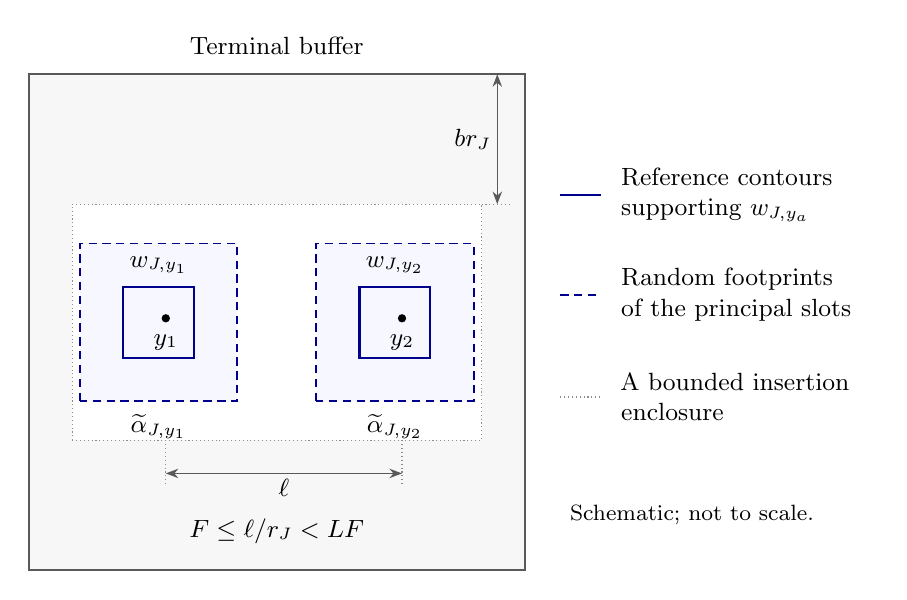
\begin{tikzpicture}[x=1cm,y=1cm,font=\small,
  contour/.style={draw=blue!55!black,line width=.8pt},
  footprint/.style={draw=blue!55!black,densely dashed,line width=.7pt},
  guide/.style={draw=black!45,densely dotted},
  dimension/.style={draw=black!65,{Stealth[length=1.6mm]}-{Stealth[length=1.6mm]}}]
  \fill[black!3] (-3.15,-3.15) rectangle (3.15,3.15);
  \fill[white] (-2.60,-1.5) rectangle (2.60,1.5);
  \draw[black!65,line width=.8pt] (-3.15,-3.15) rectangle (3.15,3.15);
  \node[anchor=south] at (0,3.28) {Terminal buffer};
  \draw[guide] (-2.60,-1.5) rectangle (2.60,1.5);

  \foreach \cx in {-1.5,1.5} {
    \draw[footprint,fill=blue!3] (\cx-1,-1) rectangle (\cx+1,1);
    \draw[contour] (\cx-.45,-.45) rectangle (\cx+.45,.45);
  }
  \fill (-1.41,.05) circle[radius=1.5pt];
  \fill (1.59,.05) circle[radius=1.5pt];
  \node[anchor=north] at (-1.41,-.03) {$y_1$};
  \node[anchor=north] at (1.59,-.03) {$y_2$};
  \node[anchor=south] at (-1.5,.50) {$w_{J,y_1}$};
  \node[anchor=south] at (1.5,.50) {$w_{J,y_2}$};
  \node[anchor=north] at (-1.5,-1.05) {$\widetilde\alpha_{J,y_1}$};
  \node[anchor=north] at (1.5,-1.05) {$\widetilde\alpha_{J,y_2}$};

  \draw[dimension] (2.80,1.5) -- (2.80,3.15)
    node[midway,left,fill=black!3,inner sep=2pt] {$b r_J$};
  \draw[guide] (2.60,1.5) -- (2.97,1.5);
  \draw[guide] (-1.41,-1.55) -- (-1.41,-2.08);
  \draw[guide] (1.59,-1.55) -- (1.59,-2.08);
  \draw[dimension] (-1.41,-1.92) -- (1.59,-1.92)
    node[midway,below,fill=black!3,inner sep=2pt] {$\ell$};
  \node at (0,-2.65) {$F\le \ell/r_J<LF$};

  \draw[contour] (3.60,1.62) -- (4.12,1.62);
  \node[anchor=west,align=left,text width=3.15cm] at (4.25,1.62)
    {Reference contours\\supporting $w_{J,y_a}$};
  \draw[footprint] (3.60,.35) -- (4.12,.35);
  \node[anchor=west,align=left,text width=3.15cm] at (4.25,.35)
    {Random footprints\\of the principal slots};
  \draw[guide] (3.60,-.95) -- (4.12,-.95);
  \node[anchor=west,align=left,text width=3.15cm] at (4.25,-.95)
    {A bounded insertion\\enclosure};
  \node[anchor=west,align=left,text width=3.7cm,font=\footnotesize]
    at (3.60,-2.45) {Schematic; not to scale.};
\end{tikzpicture}
\caption{Geometry of the terminal readout.  The solid inner squares are
the reference contours defining $w_{J,y_a}$, centered at the cells
$c_J(y_a)$.  The dashed principal footprints record the disorder and
decision seeds determining $\widetilde\alpha_{J,y_a}$; their disjointness,
including the safety layer for edge variables, gives independence of the
two amplitudes.  The dotted enclosure has bounded diameter in terminal
cell units.  A surrounding square provides margin of order $b r_J$,
where $b=J^{4/25}$.  Removing terminal interactions whose spin supports
meet this square leaves a reference conditional expectation inside it.
The two spin observables are still evaluated jointly in that
expectation.  Shapes and relative lengths are schematic.}
\label{read:geometry}
\end{figure}


Let $T_{J,N}$ be the sum of the sup norms of all
terminal background slots whose spin supports meet the buffer or its
interior.  We may bound it by the larger sum over slots whose recorded
carriers meet that region.  There are $O(b^2)$ possible cells at which
to root such a slot.  The exponential weights pay the choices of
animals and any distance of their anchors from those cells.  The
background $L^p$ bound from Proposition~\ref{flow:tuned} and Minkowski's
inequality consequently give
\begin{equation}
 \limsup_{N\to\infty}\norm{T_{J,N}}_{L^p}
    \le C b^2s_J=O_D(J^{-9/50}).
 \label{read:buffer-cost}
\end{equation}
Finite-box errors vanish by the preceding fixed-step argument.  We
have chosen the fixed background moment $p$ sufficiently large; any
$p>25$ suffices for the probability estimates below, and the earlier
construction allows much larger values.

Put $Q_J=w_{J,y_1}w_{J,y_2}$ and
$q_J=\langle Q_J\rangle_0$, where the latter is plane reference
expectation.  If $T_{J,N}\le1$, delete these background slots.
For a bounded observable and a perturbation $W$ with
$\norm W_\infty\le T$, differentiation of normalized expectations
along $\exp(tW)$, $0\le t\le1$, gives
\[
 \left|\frac{\dd}{\dd t}\langle Q\rangle_t\right|
   =|\Cov_t(Q,W)|\le2\norm Q_\infty T.
\]
Thus deletion changes the expectation of $Q_J$ by at most $CT_{J,N}$.
Conditionally on spins outside the buffer, the remaining law inside
is the reference Ising law with some boundary data.  The product
$Q_J$ is even and has bounded sup norm.  Its support diameter in
terminal units is bounded uniformly in \eqref{read:stop}.  The even
conditional reference estimate of Proposition~\ref{ref:operator}
therefore changes its expectation from the plane value by at most
$C/b$, uniformly in those outer data.  On the complementary event we
use the uniform bound $C$ on both expectations.  In particular, if
\[
 B_{J,N}=\{T_{J,N}>J^{-7/50}\},
 \qquad
 \Delta_{J,N}=\langle Q_J\rangle_{J,N,\omega}-q_J,
\]
then
\begin{equation}
 |\Delta_{J,N}|\le C(J^{-7/50}+J^{-4/25})
     \quad\hbox{on }B_{J,N}^{\mathrm c},
 \qquad |\Delta_{J,N}|\le C,
 \qquad
 \limsup_{N\to\infty}\Prob(B_{J,N})\le C_DJ^{-p/25}.
 \label{read:buffer-good}
\end{equation}
The probability bound follows from Markov's inequality and
\eqref{read:buffer-cost}; it requires no independence between
$T_{J,N}$ and the amplitudes.

Here are the distinct estimates needed for the first and second
moments.  On $B_{J,N}^{\mathrm c}$, \eqref{read:product-moments} gives
\begin{align*}
 \E\bigl[|Z_J\Delta_{J,N}|\one_{B_{J,N}^{\mathrm c}}\bigr]
     &\le J^{1/8-7/50+o(1)}=J^{-3/200+o(1)},\\
 \norm{Z_J\Delta_{J,N}\one_{B_{J,N}^{\mathrm c}}}_{L^2}
     &\le J^{1/8-7/50+o(1)}.
\end{align*}
On the exceptional event, H\"older's inequality gives, after the
finite-volume limit,
\begin{align*}
 \limsup_{N\to\infty}
 \E\bigl[|Z_J\Delta_{J,N}|\one_{B_{J,N}}\bigr]
     &\le C\norm{Z_J}_{L^2}J^{-p/50}
       =J^{1/8-p/50+o(1)},\\
 \limsup_{N\to\infty}
 \norm{Z_J\Delta_{J,N}\one_{B_{J,N}}}_{L^2}
     &\le C\norm{Z_J}_{L^4}J^{-p/100}
       =J^{3/8-p/100+o(1)}.
\end{align*}
The first error tends to zero.  For some fixed $\eta>0$ the second
is $O(J^{1/8-\eta+o(1)})$, since $p>25$.  Together with
\eqref{read:amplitude-readout}, these estimates prove
\begin{equation}
 \begin{split}
 \limsup_{N\to\infty}
 \E\left|r_J^{2d}
  \langle\sigma_{y_1}\sigma_{y_2}\rangle^{\mathrm{free}}_{N,\omega}
       -q_JZ_J\right|&=o(1),\\
 \limsup_{N\to\infty}
 \norm{r_J^{2d}
  \langle\sigma_{y_1}\sigma_{y_2}\rangle^{\mathrm{free}}_{N,\omega}
       -q_JZ_J}_{L^2}
       &=O(J^{1/8-\eta+o(1)}).
 \end{split}
 \label{read:two-errors}
\end{equation}
Decrease $\eta$ if necessary to include the joint-source error
$J^{-1/8+o(1)}$.  The separate $L^1$ estimate is useful: a relative
$L^2$ estimate alone would not recover the bounded first moment.

The two reference averaging squares defining $w_{J,y_a}$ are
disjoint.  Conditional independence in the reference model, given
their contours, and the tower property yield the exact equality
\begin{equation}
 q_J=r_J^{2d}\langle\sigma_{y_1}\sigma_{y_2}\rangle_0.
 \label{read:reference-pair}
\end{equation}
The separated reference correlation limit, uniformly over the
compact window \eqref{read:stop} and over directions, gives
$0<c\le q_J\le C$.  Thus arbitrary integer separations and grid-cell
positions are covered.

\begin{proposition}[Disorder moments at tuning]
\label{read:moments}
Let $C_{*,\omega}(y_1,y_2)$ be the free infinite-volume spin correlation
at $t_*(D)$, and let $J$ be determined by \eqref{read:stop}.  For every
fixed sufficiently small $D>0$, uniformly in the two marks as their
separation tends to infinity,
\begin{equation}
 r_J^{2d}\E C_{*,\omega}(y_1,y_2)\asymp1,
 \qquad
 r_J^{4d}\E C_{*,\omega}(y_1,y_2)^2
       =J^{1/4+o(1)}.
 \label{read:moment-conclusion}
\end{equation}
\end{proposition}

\begin{proof}
For each fixed separation, free ferromagnetic correlations increase
as the volume increases and remain in $[0,1]$.  Their limit exists,
and bounded convergence passes both disorder moments to the limit.
Here $J$ and $r_J$ are fixed during this passage.  The first line of
\eqref{read:two-errors}, \eqref{read:product-moments}, and
\eqref{read:reference-pair} give the first assertion, including a
positive lower bound.  For the second, the triangle inequality and
its reverse in $L^2$ give
\[
 \left|\norm{r_J^{2d}C_{*,\omega}(y_1,y_2)}_{L^2}
             -q_J\norm{Z_J}_{L^2}\right|
 \le O(J^{1/8-\eta+o(1)}).
\]
The main term is $J^{1/8+o(1)}$, so squaring proves the second
assertion.  All finite-volume identities hold for each choice of
seeds, whereas the original correlation depends only on the bonds.
Averaging over the seeds thus leaves the asserted disorder moments
unchanged.
\end{proof}

\subsection{A finite-box estimate with wired boundary}

The identification of the transition also needs an estimate in boxes
whose boundary is fixed to plus.  Such a boundary can create an odd
saved scalar, so it is important to keep the carrier of that scalar
until its distance from the central mark has been used.

\begin{proposition}[Wired arm at tuning]
\label{read:arm}
For any square box of radius $n$ centered at a lattice site $y$, let
$\phi^w_{n,*,\omega}$ be the FK--Ising law at $t_*(D)$ with wired
boundary.  Then
\begin{equation}
 \E\left[\phi^w_{n,*,\omega}
    (y\longleftrightarrow\partial\Lambda_n(y))^{400}\right]
       \le n^{-400/8+o(1)}.
 \label{read:arm-bound}
\end{equation}
The estimate is uniform in $y$.  It also holds if the fixed wall is
one lattice layer inside or outside the indicated square, including
the convention with bonds crossing to an exterior wired layer.
\end{proposition}

\begin{proof}
Under the Edwards--Sokal coupling~\cite{EdwardsSokal1988}, the wired
arm probability equals the spin expectation with the corresponding
plus wall.  Start a single source at $y$ and let $J_n$ be the largest
integer satisfying
\begin{equation}
 r_{J_n}\le n/(\log n)^2.
 \label{read:arm-stop}
\end{equation}
Thus $r_{J_n}\asymp n/(\log n)^2$, $J_n=O(\log n)$, and the principal
halo remains far from the wall for every $j\le J_n$.

Use the finite-box blocking rule, which forbids cuts near the wall
and leaves those interactions in the lists.  Every singleton term
whose full footprint stays in the bulk equals its plane counterpart.
By the weighted $L^{400}$ source estimate and
Proposition~\ref{mark:moments}, the sum of the sup costs of these
bulk terms at the final scale has $L^{400}$ norm bounded by a fixed
power of $1+J_n$.  Indeed
$A_{j,400}^{1/400}=j^{399/16+o(1)}$, and summing the exponential
slot weights only changes its constant.  A local odd scalar is zero:
before the boundary spins are evaluated, the bulk kernels and the
plane centering are invariant under simultaneous spin flip.

It remains to estimate all terms that can see the wall, including
saved scalar increments.  Every such source footprint contains the
mark and reaches the boundary region.  At scale $j$ its carrier length
is therefore at least $c n/r_j$.  The deterministic weighted source
transport costs a fixed factor $K$ per step, even with arbitrary
principal background sizes: selected averages are normalized, retained
large terms do not enlarge a source norm, and the small-field
coefficient sums are bounded.  This is the source estimate of
Section~\ref{sec:norms} applied without averaging over the randomness.
Keep an additional exponential carrier weight.  At each possible
scale of first boundary contact it supplies
$\exp(-c'n/r_j)$.  Sum these contributions, retaining the source
rescaling up to $J_n$; changing $K$ absorbs both that rescaling and
the sum over the possible first-contact steps.  The total deterministic
cost at the stopping scale is at most
\begin{equation}
 C K^{J_n}\exp(-c'n/r_{J_n})
 \le \exp\bigl(C\log n-c''(\log n)^2\bigr).
 \label{read:boundary-tail}
\end{equation}
One can equivalently subtract the plane and finite-box constructions:
the first coefficient where they differ must have a footprint meeting
the wall, and each later difference is transported with the same
weighted estimate.  This verifies the bound for all nonbulk
coefficients without assuming that their laws agree with plane laws.
For an odd scalar the carrier weight is used before its support is
forgotten, so \eqref{read:boundary-tail} includes all nonzero scalar
contributions.  Initial fixed constants merely change $C$.

The exact normalized one-source identity now expresses the plus
magnetization, multiplied by $r_{J_n}^d$, as the terminal expectation
of the scaled source plus its saved scalar.  Its absolute value is
bounded by the total sup costs just estimated, irrespective of the
terminal background.  Hence, for some fixed $M<\infty$,
\[
 \norm{\langle\sigma_y\rangle^+_{n,*,\omega}}_{L^{400}}
 \le r_{J_n}^{-d}\left(C(1+J_n)^M
                  +C K^{J_n}e^{-c'n/r_{J_n}}\right)
       =n^{-d+o(1)}.
\]
Raising this inequality to the power $400$ proves
\eqref{read:arm-bound}.  Translating the box changes none of the
constants because the source estimates are uniform in its mark.
Moving the wall by a bounded number of lattice layers changes the
lower bound on the boundary-reaching carrier length only by a fixed
factor, proving the remaining conventions.
\end{proof}

In particular the averaged plus magnetization vanishes at tuning.
The next section uses the stronger finite-box bound
\eqref{read:arm-bound} to identify the tuned parameter and to show
that magnetization becomes positive above it.

\section{Identification of the physical transition}
\label{sec:transition}

The construction in Proposition~\ref{flow:tuned} selects a parameter
$t_*=t_*(D)$, and Propositions~\ref{read:moments} and~\ref{read:arm}
give correlation moments and a wired one-arm estimate there.  We now show
that $t_*=0$ and that this value is the magnetization threshold.  The
first assertion uses partition functions on tori and a product-space
influence inequality.  The second uses the high moment in
Proposition~\ref{read:arm} to control a decision-tree exploration in a fixed
environment.

For a finite graph $G=(V,E)$, put $v_e=e^{2K_e}-1$ and write
\begin{equation}\label{crit:fk-law}
 \phi_{G,t,\omega}(A)
 =\frac{1}{\mathcal Z_{G,t,\omega}}
       2^{k(A)}\prod_{e\in A}v_e,
 \qquad A\subset E.
\end{equation}
Here $k(A)$ counts components of the spanning subgraph $(V,A)$; a
specified boundary wiring is imposed before counting components.
Superscripts $\mathrm f$ and $\mathrm w$ indicate free and wired
boundaries.  All these probabilities are normalized at fixed $\omega$.
The Edwards--Sokal coupling~\cite{EdwardsSokal1988} identifies the
wired connection probability to the boundary with the corresponding
plus-boundary spin expectation.  In infinite volume it gives
\begin{equation}\label{crit:magnetization}
 \langle\sigma_0\rangle^+_{t,\omega}
       =\phi^{\mathrm w}_{t,\omega}(0\longleftrightarrow\infty).
\end{equation}
Finite-energy bounds, positive association, and comparison in the
couplings hold uniformly on any fixed compact $(t,D)$ window considered
below.  In particular, for some $\eta>0$, every one-edge conditional
open probability, with any other edges prescribed, lies in
$[\eta,1-\eta]$.  This follows directly from
\eqref{crit:fk-law}: that probability is either $v_e/(1+v_e)$ or
$v_e/(2+v_e)$.

\subsection{Torus duality and twisted partition functions}

Let $\mathbb T_\ell=(\Z/\ell\Z)^2$ have its usual square cellulation.
For $A\subset E(\mathbb T_\ell)$, let
$H(A)\subset H_1(\mathbb T_\ell;\mathbb F_2)=\mathbb F_2^2$ be the
image of its cycle space, and put $r(A)=\dim H(A)$.  The complementary
dual configuration $A^*$ contains the dual of each edge outside $A$.
For each nonzero character
$\chi:\mathbb F_2^2\longrightarrow\mathbb F_2$, define the increasing,
translation-invariant event
\[
 \mathcal H_\chi=\{A:\chi|_{H(A)}\ne0\}.
\]
Thus $\mathcal H_\chi$ asks for an open cycle detected by $\chi$.

\begin{lemma}[Torus duality]\label{crit:torus-duality}
Under the intersection pairing,
\begin{equation}\label{crit:homology-annihilator}
 H(A^*)=H(A)^\perp,\qquad r(A^*)=2-r(A).
\end{equation}
If $v_{e^*}^*=2/v_e$, then complement duality carries the torus FK law
at $v$ to a measure whose density with respect to the torus FK law at
$v^*$ lies between $1/4$ and $4$.
\end{lemma}

\begin{proof}
The cycle space of $(V,A)$ has dimension $|A|-|V|+k(A)$.  A cellular
boundary is supported on $A$ precisely when its face coefficients are
constant on each complementary dual component.  The space of such
boundaries therefore has dimension $k(A^*)-1$: its face coefficients
have $k(A^*)$ degrees of freedom, and adding the constant two-chain
does not change the boundary.  Consequently
\begin{equation}\label{crit:euler}
 |A|-|V|+k(A)=k(A^*)-1+r(A).
\end{equation}
Apply the same identity on the dual cellulation and add the two
identities.  The torus Euler formula $|V|-|E|+|F|=0$ gives
$r(A)+r(A^*)=2$.  Primal and complementary dual cycles have zero
intersection, since a primal edge and its transverse dual cannot both
be present.  This inclusion, together with the dimension identity,
proves \eqref{crit:homology-annihilator}.

The ratio of the two unnormalized weights is
\begin{align*}
 \frac{2^{k(A)}\prod_{e\in A}v_e}
 {2^{k(A^*)}\prod_{e\notin A}(2/v_e)}
 &=\Big(\prod_{e\in E}v_e\Big)
            2^{k(A)-k(A^*)-|E|+|A|}\\
 &=\Big(\prod_{e\in E}v_e\Big)
            2^{|V|-|E|-1}\,2^{r(A)},
\end{align*}
where the last equality uses \eqref{crit:euler}.  The first factor is
independent of $A$, and $1\le2^{r(A)}\le4$.  Normalization proves the
claimed comparison.
\end{proof}

Choose signs $s_e^\chi\in\{-1,1\}$ representing the cocycle $\chi$,
and let $Z^\chi(K)$ be the Ising partition function with interactions
$K_es_e^\chi\sigma_x\sigma_y$.  Write $Z^0(K)$ for the ordinary
partition function.  Expanding
\[
 e^{K_es_e^\chi\sigma_x\sigma_y}
 =e^{-K_e}\bigl(1+v_e\one_{\{\sigma_x=s_e^\chi\sigma_y\}}\bigr)
\]
shows that a component of $A$ contributes two compatible spin
assignments exactly when the product of seam signs around each of its
cycles is $1$.  An incompatible component contributes zero.  Hence,
for every environment, not only after averaging,
\begin{equation}\label{crit:twist-identity}
 \frac{Z^\chi(K)}{Z^0(K)}
          =\phi_{\mathbb T_\ell,t,\omega}(\mathcal H_\chi^c).
\end{equation}

At the critical reference couplings there is $a_0>0$, independent of
$\ell$, such that
\begin{equation}\label{crit:reference-homology}
 a_0\le\phi^{\mathrm{ref}}_{\mathbb T_\ell}(\mathcal H_\chi)
                    \le1-a_0
 \qquad(\chi\ne0).
\end{equation}
For completeness, choose a coordinate generator on which $\chi$ is
nonzero.  In a narrow toric strip along that generator, a bounded
number of overlapping fixed-aspect rectangle crossings, with transverse
crossings in their overlaps, produces an open generator cycle.
The arbitrary-boundary crossing bounds of
\cite[Theorem~1.1]{CDH2016}, applied in the rectangular charts, and FK
positive association give a uniform lower bound.  Make both generator
cycles in the dual configuration in the same way.  Their homology has
rank two, so \eqref{crit:homology-annihilator} forces $H(A)=0$.
Lemma~\ref{crit:torus-duality} compares the complemented law with the
critical dual FK law by an absolute factor.  This proves the upper
bound in \eqref{crit:reference-homology}.  Only finitely many crossings
are used, so their lower bounds do not deteriorate with $\ell$.

\begin{lemma}[Transfer of torus nondegeneracy]\label{crit:torus-transfer}
Fix a sufficiently large integer $Q$.  After choosing the smallness
constants of the construction sufficiently small, there is $a_1>0$
such that, for $\ell_J=Qr_J$ and every nonzero $\chi$,
\begin{equation}\label{crit:tuned-homology}
 a_1\le \E\phi_{\mathbb T_{\ell_J},t_*,\omega}(\mathcal H_\chi)
                 \le1-a_1
\end{equation}
for all sufficiently large $J$.
\end{lemma}

\begin{proof}
Apply the exact finite-volume map of Proposition~\ref{block:finite}
to the untwisted model and to the $\chi$-twisted model, using the
corresponding critical reference partition function in each case and
the same decision seeds.  A twist is removed on a contractible chart
by a spin gauge transformation.  Every background function is even,
so the ambiguity of a simultaneous sign change on the chart does not
alter it.  Conditional reference averaging, the local decisions, and
plane centering in this gauge therefore give identical chart
coefficients and identical saved scalar increments in the two runs.

Here is why the errors outside charts remain uniform in $J$.  Choose
$Q$ larger than the fixed halos and chart margins in the construction.
A principal output uses only a short parent footprint, by
Lemma~\ref{block:carrier}.  That footprint lifts to the plane at
every scale up to $J$, and its environment and seeds have the planar
law.  A nonchart footprint has length at least $cm$ when the torus has
side $m$ at the scale carrying that footprint.  Changing between input
and output cells changes this constant by the fixed factor $L$ only.
It cannot satisfy the short-footprint rule
for a principal output.  This also proves that a seam crossing a
short footprint causes no exception: it is removed by the local
gauge, whereas a genuinely nonchart input remains in the tail.

Keep the scalar supports until applying the enhanced tree weights in
Lemma~\ref{block:tree} and Corollary~\ref{block:diameter}.
Summing the possible nonchart footprints,
including the neighborhoods used by the decisions, bounds the
uncancelled scalar increment at this step by
\[
 C_L\delta m^2e^{-cm}.
\]
There are $O(m^2)$ possible roots; the additional length weight pays
$e^{-cm}$ after the animal sum.  The side lengths $m$ decrease
geometrically and remain at least $Q$, so their total is bounded by
$C_L\delta Q^2e^{-c'Q}$, independently of $J$.  The final tail functions
have total supremum norm at most $C\delta Q^2$.  These estimates use
the finite-volume weighted bounds before forgetting supports, and
apply also to normalized conditional operations on nonchart terms.

To see precisely how these errors enter the desired ratio, let
$c_J^\chi,H_J^\chi$ denote the accumulated scalar and terminal
background for a twist, and use superscript $0$ for the untwisted
run.  Exact partition preservation gives
\begin{equation}\label{crit:terminal-ratio}
 \frac{Z^\chi(K)}{Z^0(K)}
 =\frac{Z^\chi(K^{\mathrm{ref}})}{Z^0(K^{\mathrm{ref}})}
       e^{c_J^\chi-c_J^0}
       \frac{\langle e^{H_J^\chi}\rangle_{J,\mathrm{ref},\chi}}
            {\langle e^{H_J^0}\rangle_{J,\mathrm{ref},0}}.
\end{equation}
The brackets are normalized terminal reference expectations in the
respective exact partition identities.  Chart scalar increments
cancel in $c_J^\chi-c_J^0$, leaving the nonchart bound above.
At the final scale there are only $O(Q^2)$ principal slots.  Their
laws agree in charts with the planar laws, so the high-moment bounds
along the tuned flow imply that their total supremum norm converges
to zero in probability as $J\to\infty$.  Denote this total, in the two
runs together, by $P_J$.  Exact partition preservation and
$|\log\langle e^H\rangle|\le\norm{H}_\infty$ now give
\begin{equation}\label{crit:log-ratio-transfer}
 \left|\log\frac{Z^\chi(K)/Z^0(K)}
                         {Z^\chi(K^{\mathrm{ref}})/Z^0(K^{\mathrm{ref}})}
       \right|
 \le P_J+C\delta Q^2+C_L\delta Q^2e^{-c'Q},
 \qquad P_J\xrightarrow{\Prob}0.
\end{equation}
The reference ratios here are on the same microscopic torus; exact
blocking has not replaced them by a limiting torus ratio.
First fix $Q$, then choose $\delta$ and the permitted disorder so that
the deterministic errors are smaller than a fixed tolerance depending
on $a_0$, and finally let $J$ grow.  By
\eqref{crit:twist-identity} and \eqref{crit:reference-homology}, on an
event of probability tending to one all three tuned character
probabilities lie in a common compact subinterval of $(0,1)$.
Their values always lie in $[0,1]$, so averaging proves
\eqref{crit:tuned-homology}.
\end{proof}

\subsection{Sharp thresholds after averaging the environment}

We next prove the threshold estimate needed for the torus events.
The environment is independent across bonds, but the FK edges are
not.  A monotone sequential representation lets us apply the product
influence theorem while keeping the useful derivative as a quenched
covariance.

\begin{lemma}[Torus threshold inequality]\label{crit:threshold}
Fix a compact parameter window containing $0$ and $t_*(D)$, with
uniformly positive, bounded couplings.  If $\mathcal A$ is any
increasing translation-invariant event on $\mathbb T_\ell$ and
$f_\ell(t)=\E\phi_{\mathbb T_\ell,t,\omega}(\mathcal A)$, then
\begin{equation}\label{crit:threshold-inequality}
 f_\ell'(t)\ge c\log\ell\, f_\ell(t)(1-f_\ell(t)),
 \qquad \ell\ge3,
\end{equation}
with $c>0$ independent of $\ell$ and $\mathcal A$.
\end{lemma}

\begin{proof}
For a fixed environment abbreviate its FK law to $\phi$, and set
$X_e=\one_{\{e\in A\}}$ and
$c_e(\omega)=\Cov_{\phi_{t,\omega}}(\one_{\mathcal A},X_e)\ge0$.
Differentiating the finite sum in \eqref{crit:fk-law} gives
\begin{equation}\label{crit:derivative}
 f_\ell'(t)=\sum_e\E[\lambda_e(t,\omega)c_e(\omega)],
 \qquad
 \lambda_e=\frac{\dd}{\dd t}\log v_e.
\end{equation}
Since $\dd K_e/\dd t=\tfrac12\tanh(2K_e)$, the coefficients
$\lambda_e=\tanh(2K_e)e^{2K_e}/(e^{2K_e}-1)$ have uniform positive
lower and upper bounds.

Represent each environment bit by a uniform variable $V_e$, with
$\xi_e=1$ when $V_e\ge1/2$.  Order the FK edges arbitrarily as
$e_1,\ldots,e_M$ and use further independent uniforms $U_i$ to set
\[
 X_{e_i}=\one_{\{U_i\ge1-p_i\}},\qquad
 p_i=\phi_{t,\omega}(X_{e_i}=1\mid X_{e_1},\ldots,X_{e_{i-1}}).
\]
The conditional FK laws are increasing both in the prescribed past
and in the couplings.  Induction in $i$ therefore makes the entire
sample increasing in all the $U_i$ and $V_e$.  Let $F$ be the Boolean
indicator of $\mathcal A$ in this product representation.  For one
uniform coordinate $z$, its influence $I_z$ is the probability, over
all other coordinates, that the section of $F$ in $z$ has values zero
and one on sets of positive Lebesgue measure.

We first bound an FK-uniform influence.  Fix the environment and let
$P=(X_{e_1},\ldots,X_{e_{i-1}})$ be the past.  Write
\[
 p(P)=\phi(X_{e_i}=1\mid P),\qquad
 a_b(P)=\phi(\mathcal A\mid P,X_{e_i}=b),\quad b=0,1.
\]
The future uniforms couple the two branches monotonically.  As both
intervals for $X_{e_i}$ have length at least $\eta$, the section in
$U_i$ is nonconstant exactly when the two resulting Boolean outputs
differ.  Averaging those future uniforms gives $a_1(P)-a_0(P)$.
Consequently
\begin{align}
 I_{U_i}
 &=\E\,\phi\bigl(a_1(P)-a_0(P)\bigr)\nonumber\\
 &\le\frac{1}{\eta(1-\eta)}
       \E\,\phi\bigl(\Cov_\phi(\one_{\mathcal A},X_{e_i}\mid P)\bigr)
 \le C\E c_{e_i}(\omega).\label{crit:uniform-influence}
\end{align}
For the last inequality, total covariance gives an additional term
\[
 \Cov_\phi\bigl(\phi(\mathcal A\mid P),
                        \phi(X_{e_i}=1\mid P)\bigr)\ge0.
\]
Both functions are increasing in $P$, and the marginal distribution
of $P$ is positively associated.  This proves the indicated sign.

For the environment coordinate $V_e$, condition on every other bond.
Let $\phi_-$ and $\phi_+$ be the FK laws with its low and high value,
and put $R=v_e^+/v_e^-\ge1$.  Changing this bond multiplies the weight
by $R^{X_e}$, so direct normalization gives
\begin{equation}\label{crit:bond-tilt}
 \phi_+(\mathcal A)-\phi_-(\mathcal A)
 =\frac{(R-1)\Cov_{\phi_-}(\one_{\mathcal A},X_e)}
              {1+(R-1)\phi_-(X_e)}.
\end{equation}
Monotonicity of the common-uniform coupling makes the left side the
conditional influence of $V_e$.  The ratio $R$ is uniformly bounded.
After averaging the other bonds, the low-bond covariance is at most
twice $\E c_e(\omega)$, since both low- and high-bond covariances are
nonnegative.  Thus $I_{V_e}\le C\E c_e(\omega)$ as well.

Translation invariance of the averaged law and of $\mathcal A$ makes
$\E c_e(\omega)$ constant within each of the two edge orientations.
Each orientation has $\ell^2$ edges.  Equation~\eqref{crit:derivative}
therefore implies
\begin{equation}\label{crit:max-influence}
 \max_z I_z\le C\ell^{-2}f_\ell'(t).
\end{equation}
There is no symmetry requirement on the chosen ordering or the
sequential sampler: only the averaged covariances were compared by
translation.  There are $N=2M=4\ell^2$ product coordinates.  The BKKKL
inequality~\cite{BKKKL1992}, in the null-set-invariant formulation
\cite[Theorem~2.3 and Equation~(2.3)]{GJN2013}, gives
\[
 \max_z I_z\ge c f_\ell(t)(1-f_\ell(t))\frac{\log N}{N}.
\]
Combine this with \eqref{crit:max-influence} to obtain
\eqref{crit:threshold-inequality}.
\end{proof}

\begin{proposition}\label{crit:tuning-zero}
For every sufficiently small fixed $D>0$, the tuned parameter is
$t_*(D)=0$.
\end{proposition}

\begin{proof}
The dual transformation $v_{e^*}^*=2/v_e$ is equivalent to
$\sinh(2K_e)\sinh(2K_{e^*}^*)=1$.  Thus, in the coordinates
\eqref{eq:model-td}, it sends $(t,D,\xi)$ to $(-t,D,-\xi)$ on the dual
lattice.  At $t=0$ the environment law is invariant.  Write
$a_i=\E\phi_{\mathbb T_\ell,0,\omega}(r(A)=i)$.
Lemma~\ref{crit:torus-duality} gives
$a_0/4\le a_2\le4a_0$.  In particular,
$a_1+a_2\ge1/5$ and $a_0+a_1\ge1/5$.

There are three nonzero characters of $\mathbb F_2^2$.  A one-dimensional
homology space is detected by two of them, whereas a two-dimensional
space is detected by all three.  Therefore
\begin{align*}
 \sum_{\chi\ne0}\E\phi_{0,\omega}(\mathcal H_\chi)
      &=2a_1+3a_2,\\
 \sum_{\chi\ne0}\E\phi_{0,\omega}(\mathcal H_\chi^c)
      &=3a_0+a_1.
\end{align*}
It follows that at $t=0$ at least one character has probability bounded
below by an absolute positive constant, and at least one has
probability bounded away from one.  The two characters need not be
the same.

Apply Lemma~\ref{crit:threshold} to each $\mathcal H_\chi$ along
$\ell_J=Qr_J$.  On $(0,1)$ it states
\[
 \frac{\dd}{\dd t}\log\frac{f_{\ell_J}(t)}{1-f_{\ell_J}(t)}
                         \ge c\log\ell_J.
\]
If $t_*>0$, integrate from $0$ to $t_*$ and use the upper bound in
\eqref{crit:tuned-homology}.  Every character probability at zero
would tend to zero.  If $t_*<0$, integrate from $t_*$ to zero and use
the lower bound in \eqref{crit:tuned-homology}; every character
probability at zero would tend to one.  Both conclusions contradict
the preceding absolute bounds.  Hence $t_*=0$.
\end{proof}

\subsection{Arm decay below zero and percolation above zero}

Proposition~\ref{read:arm} and Proposition~\ref{crit:tuning-zero} already
imply zero plus magnetization at $t=0$.  The next argument extracts a
stronger consequence strictly below zero.  It applies the monotone
OSSS inequality in each good environment, so it does not require a
sharpness theorem for a translation-invariant deterministic coupling
field.

\begin{lemma}[Averaged subcritical arm bound]\label{crit:subcritical-arm}
For every fixed $t'<0$ in the parameter window and sufficiently small
fixed $D>0$,
\begin{equation}\label{crit:subcritical-decay}
 \E\phi^{\mathrm w}_{t',\omega}
                  (0\longleftrightarrow\partial\Lambda_n)
                      \le C_{t',D}n^{-6}.
\end{equation}
\end{lemma}

\begin{proof}
Put $m=\lfloor n^{1/2}\rfloor$ and, for $z\in\Lambda_{2n}$, define
\[
 q_z(\omega)=\phi^{\mathrm w}_{z+\Lambda_m,0,\omega}
           (z\longleftrightarrow z+\partial\Lambda_m).
\]
Use the wall convention of Proposition~\ref{read:arm}; shifting the wall
one lattice step does not affect its uniform estimate.  Let
$\mathcal G_n=\{q_z\le n^{-1/50}\text{ for every }z\in\Lambda_{2n}\}$.
Markov's inequality, the $400$th moment in Proposition~\ref{read:arm},
and a union bound give
\begin{align}\label{crit:exception}
 \Prob(\mathcal G_n^c)
 &\le Cn^2 n^{400/50}m^{-400/8+o(1)}
   =n^{-15+o(1)}\le Cn^{-6}.
\end{align}
All boxes use the same global environment; independence of these
box events is unnecessary.  On $\mathcal G_n$, the same inequalities
hold throughout $t\in[t',0]$ by monotonicity in $t$.

Fix such an environment, and consider
\[
 f_\omega(t)=\phi^{\mathrm w}_{\Lambda_{4n},t,\omega}(\mathcal A_n),
 \qquad
 \mathcal A_n=\{0\longleftrightarrow\partial\Lambda_n
                        \text{ by a path in }\Lambda_n\}.
\]
Choose $k$ uniformly from $\{1,\ldots,n\}$, independently of the FK
configuration.  Explore all open components in $\Lambda_n$ meeting
its square shell $\partial\Lambda_k$, revealing all edges of the
induced graph on $\Lambda_n$ incident to the vertices reached.
Retain their actual connectivity; the shell
vertices are not identified with one another.  Every path witnessing
$\mathcal A_n$ meets the chosen shell, and its whole open component
is explored.  Thus this algorithm determines $\mathcal A_n$.

For an edge $e=xy$ within $\Lambda_n$, the chance that the chosen shell
lies within distance $m+2$ of $x$ or $y$ is at most $Cm/n$.  Otherwise,
querying $e$ requires that one endpoint is already joined to the shell
by a revealed open path, and hence has an open arm of radius $m$.
The endpoint box is contained in $\Lambda_{4n}$.  Conditional on all
edges outside that box, the domain Markov property gives an induced
boundary partition, dominated by full wiring.  Its conditional arm
probability is consequently at most $q_x$ or $q_y$, uniformly for
$t\in[t',0]$.  The revealment $\delta_e(t)$ therefore satisfies
\begin{equation}\label{crit:revealment}
 \max_e\delta_e(t)
          \le C(n^{-1/2}+n^{-1/50})\le Cn^{-1/50}.
\end{equation}
Edges outside $\Lambda_n$ are never queried.

The monotone-measure OSSS inequality
\cite[Theorem~1.1]{DCRT2019}, averaged over the independent choice of
shell, gives
\[
 f_\omega(t)(1-f_\omega(t))
 \le\sum_e\delta_e(t)
       \Cov_{\phi^{\mathrm w}_{\Lambda_{4n},t,\omega}}
                         (\one_{\mathcal A_n},X_e).
\]
The shell construction is the exploration underlying
\cite[Lemma~3.2]{DCRT2019}; here its revealment is bounded using the
quenched local arms on $\mathcal G_n$.  Differentiating the FK weights
as in \eqref{crit:derivative} and using their positive lower derivative
bound yields
\[
 f_\omega'(t)\ge c n^{1/50}f_\omega(t)(1-f_\omega(t)).
\]
The event that all four edges incident to zero are closed has
probability at least $\eta^4$, by sequential conditioning and finite
energy.  Hence $f_\omega(0)\le1-\eta^4$.  Integration of the preceding
logit inequality gives
\[
 f_\omega(t')\le C\exp\{-c|t'|n^{1/50}\}.
\]
After averaging, \eqref{crit:exception} contributes at most $Cn^{-6}$.
Finally, the restriction of the infinite wired law to this cylinder
event is dominated by the wired law in $\Lambda_{4n}$, by domain
comparison.  This proves \eqref{crit:subcritical-decay}.
\end{proof}

\begin{proposition}[Transition in the $(t,D)$ coordinates]
\label{crit:identification}
For every sufficiently small fixed $D>0$, the disorder-averaged plus
magnetization vanishes at $t\le0$ and is positive at every $t>0$.
\end{proposition}

\begin{proof}
At zero, Proposition~\ref{read:arm} implies
$\E\phi^{\mathrm w}_{\Lambda_n,0,\omega}
 (0\longleftrightarrow\partial\Lambda_n)\to0$ by H\"older's
inequality.  Equations~\eqref{crit:magnetization} and monotonicity give
zero magnetization for $t\le0$.

Fix $s>0$ small enough that $-s$ lies in the parameter window.  Planar
free/wired duality sends the infinite free FK law at $(s,D,\xi)$ to
the infinite wired dual law at $(-s,D,-\xi)$.  This identity follows
first from the finite planar bond expansion and then by taking free
and wired limits; see also the boundary conventions in
\cite[Section~2.5]{CDH2016}.  The dual environment still has the same
independent binary law.  Failure of a primal crossing of a
fixed-aspect rectangle of diameter comparable to $n$ entails a dual
crossing in the transverse direction, and hence a dual arm of length
at least $cn$ from a vertex in that rectangle.  There are $O(n^2)$
possible vertices.  Lemma~\ref{crit:subcritical-arm}, translated to
each such vertex and applied at $-s$, therefore bounds the averaged
failure probability by $Cn^{-4}$.

For each $n=2^kn_0$, use the four rectangular sides of
$\Lambda_{2n}\setminus\Lambda_n$, each of width $n$ and length $4n$.
Their longitudinal crossings intersect in the corner squares and
contain an open circuit surrounding $\Lambda_n$.  Require also a
left--right crossing of
$[n/2,5n]\times[-n/4,n/4]$.  Its initial point lies inside
$\Lambda_n$ and its endpoint lies outside $\Lambda_{4n}$, so it must
intersect both this circuit and the circuit at scale $2n$.  Rounding
rectangle endpoints by a lattice step is harmless; one may choose
$n_0$ divisible by four.  All aspect ratios are fixed and there are
five requested crossings per scale.  The probability that any of
them fails is at most
\[
 C\sum_{k\ge0}(2^kn_0)^{-4},
\]
which is smaller than one for large $n_0$.  On the complementary event
the joined circuits form an infinite open connected set.  Thus the
joint law obtained by first sampling the environment and then its
infinite free FK configuration has positive probability of an infinite
cluster.  This joint law is translation stationary.  If the origin
had zero probability of belonging to an infinite cluster, every
vertex would have probability zero, and countable subadditivity would
exclude an infinite cluster anywhere.  Hence the origin has positive
connection probability.  Wired domination and
\eqref{crit:magnetization} give positive averaged plus magnetization
at $s$.  Monotonicity extends this conclusion to every $t>0$.
\end{proof}

\subsection{The physical inverse temperature and the correlation ratio}

We finish by matching the parameter just identified to the original
bonds $1+\eps\xi_e$.  For $\eps\in(0,1)$ define
\[
 b_\pm(\beta,\eps)
       =\log\sinh\bigl(2\beta(1\pm\eps)\bigr).
\]
The mean $(b_++b_-)/2$ is continuous and strictly increasing from
$-\infty$ to $+\infty$ as $\beta$ runs through $(0,\infty)$.  It has
a unique zero $\beta_*(\eps)$, characterized by
\begin{equation}\label{crit:physical-equation}
 \sinh\bigl(2\beta_*(\eps)(1+\eps)\bigr)
 \sinh\bigl(2\beta_*(\eps)(1-\eps)\bigr)=1.
\end{equation}
Continuity and strict monotonicity imply
$\beta_*(\eps)\to\beta_0$ as $\eps\to0$.  At this parameter
put
\[
 D_*(\eps)=\tfrac12
       \bigl(b_+(\beta_*,\eps)-b_-(\beta_*,\eps)\bigr).
\]
Then $D_*(\eps)>0$ for $\eps>0$ and
$D_*(\eps)\to0$.  Choose $\eps_0>0$ so that this value belongs
to the permitted disorder interval whenever $0<\eps<\eps_0$.
At $\beta_*$ the physical model is exactly $(t,D)=(0,D_*)$.
Proposition~\ref{crit:identification} makes its magnetization zero;
monotonicity gives the same conclusion below $\beta_*$.

If $\beta>\beta_*$, both increments
$b_\pm(\beta,\eps)-b_\pm(\beta_*,\eps)$ are strictly positive.
Choose $s>0$, inside the parameter window, smaller than their minimum.
With the same environment, the physical couplings at $\beta$ dominate
those with log-sinh values $s+D_*\xi_e$.  The latter model has positive
averaged magnetization by Proposition~\ref{crit:identification}.
Consequently
\begin{equation}\label{crit:physical-beta}
 \beta_c(\eps)=\beta_*(\eps),
 \qquad m_\eps(\beta_c(\eps))=0.
\end{equation}
This comparison keeps $D_*$ fixed; no assumption about holding the
physical log-sinh difference constant while varying $\beta$ is used.

\begin{proof}[Proof of Theorem~\ref{thm:main}]
Fix $\eps\in(0,\eps_0)$ and use $D=D_*(\eps)>0$.
By \eqref{crit:physical-beta} and Proposition~\ref{crit:tuning-zero},
the tuned free infinite-volume correlation of
Proposition~\ref{read:moments} is $C_{\eps,\omega}(r)$ at the physical
critical inverse temperature.  That proposition gives, at its stopping
scale $J=\log r/\log L+O(1)$,
\[
 r_J^{2d}\E C_{\eps,\omega}(r)\asymp1,
 \qquad
 r_J^{4d}\E C_{\eps,\omega}(r)^2=J^{1/4+o(1)}.
\]
The factors $r_J^{4d}$ cancel in the ratio of the second moment to the
square of the first.  Thus
\[
 \log R_\eps(r)=(1/4+o(1))\log J+O(1),
 \qquad
 \frac{\log J}{\log\log r}\longrightarrow1,
\]
which proves the asserted limit along all integer $r\to\infty$.
The disorder remains fixed throughout this final limit.  The
thermodynamic limits and the separate Gibbs normalizations required
in the definition of $R_\eps$ are those already established in
Proposition~\ref{read:moments}.
\end{proof}

\begin{thebibliography}{99}

\bibitem{AizenmanWehr1990}
M.~Aizenman and J.~Wehr,
\emph{Rounding effects of quenched randomness on first-order phase transitions},
Communications in Mathematical Physics \textbf{130} (1990), 489--528.\newline
\href{https://doi.org/10.1007/BF02096933}{doi:10.1007/BF02096933}.

\bibitem{AGG2023}
G.~Antinucci, A.~Giuliani, and R.~L.~Greenblatt,
\emph{Energy correlations of non-integrable Ising models: The scaling
limit in the cylinder},
Communications in Mathematical Physics \textbf{397} (2023), 393--483.
\href{https://doi.org/10.1007/s00220-022-04481-z}{doi:10.1007/s00220-022-04481-z}.

\bibitem{BKKKL1992}
J.~Bourgain, J.~Kahn, G.~Kalai, Y.~Katznelson, and N.~Linial,
\emph{The influence of variables in product spaces},
Israel Journal of Mathematics \textbf{77} (1992), nos.~1--2, 55--64.
\href{https://doi.org/10.1007/BF02808010}{doi:10.1007/BF02808010}.

\bibitem{CGG2025}
G.~Cava, A.~Giuliani, and R.~L.~Greenblatt,
\emph{The scaling limit of boundary spin correlations in non-integrable
Ising models},
Journal of Mathematical Physics \textbf{66} (2025), no.~2, 023301.
\href{https://doi.org/10.1063/5.0235381}{doi:10.1063/5.0235381}.

\bibitem{ChayesShtengel1999}
L.~Chayes and K.~Shtengel,
\emph{Critical behavior for 2D uniform and disordered ferromagnets
at self-dual points},
Communications in Mathematical Physics \textbf{204} (1999), 353--366.
\href{https://doi.org/10.1007/s002200050649}{doi:10.1007/s002200050649}.
\href{https://arxiv.org/abs/cond-mat/9811203}{arXiv:cond-mat/9811203}.

\bibitem{CDH2016}
D.~Chelkak, H.~Duminil-Copin, and C.~Hongler,
\emph{Crossing probabilities in topological rectangles for the
critical planar FK-Ising model},
Electronic Journal of Probability \textbf{21} (2016), paper no.~5, 1--28.
\href{https://doi.org/10.1214/16-EJP3452}{doi:10.1214/16-EJP3452}.
\href{https://arxiv.org/abs/1312.7785}{arXiv:1312.7785}.

\bibitem{CHI2015}
D.~Chelkak, C.~Hongler, and K.~Izyurov,
\emph{Conformal invariance of spin correlations in the planar Ising model},
Annals of Mathematics \textbf{181} (2015), no.~3, 1087--1138.\newline
\href{https://doi.org/10.4007/annals.2015.181.3.5}{doi:10.4007/annals.2015.181.3.5}.

\bibitem{CHI2023}
D.~Chelkak, C.~Hongler, and K.~Izyurov,
\emph{Correlations of primary fields in the critical Ising model},
preprint, 2021; revised 23 February 2022,
\href{https://arxiv.org/abs/2103.10263v2}{arXiv:2103.10263v2}.

\bibitem{DotsenkoDotsenko1983}
Vik.~S.~Dotsenko and Vl.~S.~Dotsenko,
\emph{Critical behaviour of the phase transition in the 2D Ising model
with impurities},
Advances in Physics \textbf{32} (1983), no.~2, 129--172.
\href{https://doi.org/10.1080/00018738300101541}{doi:10.1080/00018738300101541}.

\bibitem{DHN2011}
H.~Duminil-Copin, C.~Hongler, and P.~Nolin,
\emph{Connection probabilities and RSW-type bounds for the
two-dimensional FK Ising model},
Communications on Pure and Applied Mathematics \textbf{64} (2011),
no.~9, 1165--1198.
\href{https://doi.org/10.1002/cpa.20370}{doi:10.1002/cpa.20370}.

\bibitem{DCRT2019}
H.~Duminil-Copin, A.~Raoufi, and V.~Tassion,
\emph{Sharp phase transition for the random-cluster and Potts models
via decision trees},
Annals of Mathematics \textbf{189} (2019), no.~1, 75--99.
\href{https://doi.org/10.4007/annals.2019.189.1.2}{doi:10.4007/annals.2019.189.1.2}.
\href{https://arxiv.org/abs/1705.03104v2}{arXiv:1705.03104v2}.

\bibitem{EdwardsSokal1988}
R.~G.~Edwards and A.~D.~Sokal,
\emph{Generalization of the Fortuin--Kasteleyn--Swendsen--Wang
representation and Monte Carlo algorithm},
Physical Review D \textbf{38} (1988), no.~6, 2009--2012.
\href{https://doi.org/10.1103/PhysRevD.38.2009}{doi:10.1103/PhysRevD.38.2009}.

\bibitem{FK1972}
C.~M.~Fortuin and P.~W.~Kasteleyn,
\emph{On the random-cluster model: I. Introduction and relation to other
models},
Physica \textbf{57} (1972), no.~4, 536--564.
\href{https://doi.org/10.1016/0031-8914(72)90045-6}{doi:10.1016/0031-8914(72)90045-6}.

\bibitem{GGM2012}
A.~Giuliani, R.~L.~Greenblatt, and V.~Mastropietro,
\emph{The scaling limit of the energy correlations in non-integrable
Ising models},
Journal of Mathematical Physics \textbf{53} (2012), no.~9, 095214.
\href{https://doi.org/10.1063/1.4745910}{doi:10.1063/1.4745910}.

\bibitem{GJN2013}
G.~R.~Grimmett, S.~Janson, and J.~R.~Norris,
\emph{Influence in product spaces},
Advances in Applied Probability \textbf{48} (2016), special issue~A,
145--152.
\href{https://doi.org/10.1017/apr.2016.46}{doi:10.1017/apr.2016.46}.
\href{https://arxiv.org/abs/1207.1780v2}{arXiv:1207.1780v2}.

\bibitem{Harris1974}
A.~B.~Harris,
\emph{Effect of random defects on the critical behaviour of Ising models},
Journal of Physics C: Solid State Physics \textbf{7} (1974), no.~9,
1671--1692.
\href{https://doi.org/10.1088/0022-3719/7/9/009}{doi:10.1088/0022-3719/7/9/009}.

\bibitem{Ludwig1990}
A.~W.~W.~Ludwig,
\emph{Infinite hierarchies of exponents in a diluted ferromagnet and
their interpretation},
Nuclear Physics B \textbf{330} (1990), nos.~2--3, 639--680.
\href{https://doi.org/10.1016/0550-3213(90)90126-X}{doi:10.1016/0550-3213(90)90126-X}.

\bibitem{OSSS2005}
R.~O'Donnell, M.~Saks, O.~Schramm, and R.~A.~Servedio,
\emph{Every decision tree has an influential variable},
Proceedings of the 46th Annual IEEE Symposium on Foundations of
Computer Science (2005), 31--39.
\href{https://doi.org/10.1109/SFCS.2005.34}{doi:10.1109/SFCS.2005.34}.
\href{https://arxiv.org/abs/cs/0508071}{arXiv:cs/0508071}.

\bibitem{ReferenceIsing}
OpenAI,
\emph{Conformal universality of bulk Ising correlations under weak interactions},
OpenAI Math Release preprint
\href{https://github.com/openai/math/blob/main/preprints/Conformal-universality-of-bulk-Ising-correlations-under-weak-interactions-September-23-2026/paper.pdf}{OAI:Conformal-universality-of-bulk-Ising-correlations-under-weak-interactions-September-23-2026},
2026.
Theorem~1.1; Lemmas~2.1, 3.3, 4.5, and~5.3;
Corollary~2.2; Propositions~4.1, 5.2, and~5.4; Equation~(5.18).

\bibitem{Shalaev1984}
B.~N.~Shalaev,
\emph{Correlation function and susceptibility of a two-dimensional
Ising model with impurities},
Fizika Tverdogo Tela \textbf{26} (1984), no.~10, 3002--3005 (in Russian).

\bibitem{Shankar1987}
R.~Shankar,
\emph{Exact critical behavior of a random bond two-dimensional Ising model},
Physical Review Letters \textbf{58} (1987), 2466--2469;
erratum, \textbf{59} (1987), 380.
\href{https://doi.org/10.1103/PhysRevLett.58.2466}{doi:10.1103/PhysRevLett.58.2466};
\href{https://doi.org/10.1103/PhysRevLett.59.380.2}{doi:10.1103/PhysRevLett.59.380.2}.

\end{thebibliography}

\end{document}
